% !TeX spellcheck = russian-aot-ieyo
% Зачем: Определяет класс документа (То, как будет выглядеть документ)
% Примечание: параметр draft помечает строки, вышедшие за границы страницы, прямоугольником, в фильной версии его нужно удалить.
\documentclass[a4paper,14pt,russian,oneside,final]{extreport}

% Зачем: Настройка Times New Roman.
% Рекомендовано для Windows (нужен PSCyr, подробности см. в fonts_windows.tex)
% раскомментировать, чтобы использовать:
% Зачем: Предоставляет проприетарный Times New Roman.
% ОБНОВЛЕНИЕ: лучше использовать scalable-cyrfonts-tex: меньше проблем с установкой
% Из руководства к PSCyr: "Во избежание проблем пакет PSCyr должен загружаться перед пакета-ми inputenc и babel".
% Примечание: Требует шаманства при установке, инструкция http://plumbum-blog.blogspot.com/2010/06/miktex-28-pscyr-04d.html
% http://blog.harrix.org/?p=444
\usepackage{pscyr}

% Зачем: Выбор внутренней TeX кодировки.
\usepackage[T2A]{fontenc}

% не забудьте закомментировать % Зачем: Выбор внутренней TeX кодировки.
\usepackage[T2A]{fontenc}

% Зачем: Предоставляет свободный Times New Roman.
% Шрифт идёт вместе с пакетом scalable-cyrfonts-tex в Ubuntu/Debian

% пакет scalable-cyrfonts-tex может конфликтовать с texlive-fonts-extra в Ubuntu
% решение: Для себя я решил эту проблему так: пересобрал пакет scalable-cyrfonts-tex, изменив его имя. Решение топорное, но работает. Желающие могут скачать мой пакет здесь:
% https://yadi.sk/d/GW2PhDgEcJH7m
% Установка:
% dpkg -i scalable-cyrfonts-tex-shurph_4.16_all.deb

\usefont{T2A}{ftm}{m}{sl}


% Рекомендовано для Linux (нужен scalable-cyrfonts-tex, подробности см. в fonts_linux.tex)
% раскомментировать, чтобы использовать:
%% Зачем: Выбор внутренней TeX кодировки.
\usepackage[T2A]{fontenc}

% Зачем: Предоставляет свободный Times New Roman.
% Шрифт идёт вместе с пакетом scalable-cyrfonts-tex в Ubuntu/Debian

% пакет scalable-cyrfonts-tex может конфликтовать с texlive-fonts-extra в Ubuntu
% решение: Для себя я решил эту проблему так: пересобрал пакет scalable-cyrfonts-tex, изменив его имя. Решение топорное, но работает. Желающие могут скачать мой пакет здесь:
% https://yadi.sk/d/GW2PhDgEcJH7m
% Установка:
% dpkg -i scalable-cyrfonts-tex-shurph_4.16_all.deb

\usefont{T2A}{ftm}{m}{sl}
% не забудьте закомментировать % Зачем: Предоставляет проприетарный Times New Roman.
% ОБНОВЛЕНИЕ: лучше использовать scalable-cyrfonts-tex: меньше проблем с установкой
% Из руководства к PSCyr: "Во избежание проблем пакет PSCyr должен загружаться перед пакета-ми inputenc и babel".
% Примечание: Требует шаманства при установке, инструкция http://plumbum-blog.blogspot.com/2010/06/miktex-28-pscyr-04d.html
% http://blog.harrix.org/?p=444
\usepackage{pscyr}

% Зачем: Выбор внутренней TeX кодировки.
\usepackage[T2A]{fontenc}



% Зачем: Установка кодировки исходных файлов.
\usepackage[utf8]{inputenc}
\usepackage{csquotes}

% Зачем: Делает результирующий PDF "searchable and copyable".
\usepackage{cmap}

% Зачем: Чтобы можно было использовать русские буквы в формулах, но в случае использования предупреждать об этом.
\usepackage[warn]{mathtext}

% Зачем: Учет особенностей различных языков.
\usepackage[russian]{babel}
\usepackage{float}

% Зачем: Добавляет поддержу дополнительных размеров текста 8pt, 9pt, 10pt, 11pt, 12pt, 14pt, 17pt, and 20pt.
% Почему: Пункт 2.1.1 Требований по оформлению пояснительной записки.
\usepackage{extsizes}


% Зачем: Длинна, пимерно соответвующая 5 символам
% Почему: Требования содержат странное требование про отсупы в 5 символов (для немоноширинного шрифта :| )
\newlength{\fivecharsapprox}
\setlength{\fivecharsapprox}{6ex}


% Зачем: Добавляет отступы для абзацев.
% Почему: Пункт 2.1.3 Требований по оформлению пояснительной записки.
\usepackage{indentfirst}
\setlength{\parindent}{\fivecharsapprox} % Примерно соответсвует 5 символам.


% Зачем: Настраивает отступы от границ страницы.
% Почему: Пункт 2.1.2 Требований по оформлению пояснительной записки.
\usepackage[left=3cm,top=2.0cm,right=1.5cm,bottom=2.7cm]{geometry}


% Зачем: Настраивает межстрочный интервал, для размещения 40 +/- 3 строки текста на странице.
% Почему: Пункт 2.1.1 Требований по оформлению пояснительной записки.
\usepackage[nodisplayskipstretch]{setspace} 
\setstretch{1.1}
%\onehalfspacing

% Зачем: Выбор шрифта по-умолчанию. 
% Почему: Пункт 2.1.1 Требований по оформлению пояснительной записки.
% Примечание: В требованиях не указан, какой именно шрифт использовать. По традиции используем TNR.
\renewcommand{\rmdefault}{ftm} % Times New Roman


% Зачем: Отключает использование изменяемых межсловных пробелов.
% Почему: Так не принято делать в текстах на русском языке.
\frenchspacing


% Зачем: Сброс счетчика сносок для каждой страницы
% Примечание: в "Требованиях по оформлению пояснительной записки" не указано, как нужно делать, но в других БГУИРовских докуметах рекомендуется нумерация отдельная для каждой страницы
\usepackage{perpage}
\MakePerPage{footnote}


% Зачем: Добавляет скобку 1) к номеру сноски
% Почему: Пункты 2.9.2 и 2.9.1 Требований по оформлению пояснительной записки.
\makeatletter 
\def\@makefnmark{\hbox{\@textsuperscript{\normalfont\@thefnmark)}}}
\makeatother


% Зачем: Расположение сносок внизу страницы
% Почему: Пункт 2.9.2 Требований по оформлению пояснительной записки.
\usepackage[bottom]{footmisc}


% Зачем: Переопределяем стандартную нумерацию, т.к. в отчете будут только section и т.д. в терминологии TeX
\makeatletter
\renewcommand{\thesection}{\arabic{section}}
\makeatother


% Зачем: Пункты (в терминологии требований) в терминологии TeX subsubsection должны нумероваться
% Почему: Пункт 2.2.3 Требований по оформлению пояснительной записки.
\setcounter{secnumdepth}{3}


% Зачем: Настраивает отступ между таблицей с содержанимем и словом СОДЕРЖАНИЕ
% Почему: Пункт 2.2.7 Требований по оформлению пояснительной записки.
\usepackage{tocloft}
\setlength{\cftbeforetoctitleskip}{-1em}
\setlength{\cftaftertoctitleskip}{1em}


% Зачем: Определяет отступы слева для записей в таблице содержания.
% Почему: Пункт 2.2.7 Требований по оформлению пояснительной записки.
\makeatletter
\renewcommand{\l@section}{\@dottedtocline{1}{0.5em}{1.2em}}
\renewcommand{\l@subsection}{\@dottedtocline{2}{1.7em}{2.0em}}
\renewcommand{\l@subsubsection}{\@dottedtocline{2}{2.9em}{2.8em}}
\makeatother


% Зачем: Работа с колонтитулами
\usepackage{fancyhdr} % пакет для установки колонтитулов
\pagestyle{fancy} % смена стиля оформления страниц


% Зачем: Нумерация страниц располагается справа снизу страницы
% Почему: Пункт 2.2.8 Требований по оформлению пояснительной записки.
\fancyhf{} % очистка текущих значений
\fancyfoot[R]{\thepage} % установка верхнего колонтитула
\renewcommand{\footrulewidth}{0pt} % убрать разделительную линию внизу страницы
\renewcommand{\headrulewidth}{0pt} % убрать разделительную линию вверху страницы
\fancypagestyle{plain}{ 
    \fancyhf{}
    \rfoot{\thepage}}


% Зачем: Задает стиль заголовков раздела жирным шрифтом, прописными буквами, без точки в конце
% Почему: Пункты 2.1.1, 2.2.5, 2.2.6 и ПРИЛОЖЕНИЕ Л Требований по оформлению пояснительной записки.
\makeatletter
\renewcommand\section{%
  \clearpage\@startsection {section}{1}%
    {\fivecharsapprox}%
    {-1em \@plus -1ex \@minus -.2ex}%
    {1em \@plus .2ex}%
    {\raggedright\hyphenpenalty=10000\normalfont\large\bfseries\MakeUppercase}}
\makeatother


% Зачем: Задает стиль заголовков подразделов
% Почему: Пункты 2.1.1, 2.2.5 и ПРИЛОЖЕНИЕ Л Требований по оформлению пояснительной записки.
\makeatletter
\renewcommand\subsection{%
  \@startsection{subsection}{2}%
    {\fivecharsapprox}%
    {-1em \@plus -1ex \@minus -.2ex}%
    {1em \@plus .2ex}%
    {\raggedright\hyphenpenalty=10000\normalfont\normalsize\bfseries}}
\makeatother


% Зачем: Задает стиль заголовков пунктов
% Почему: Пункты 2.1.1, 2.2.5 и ПРИЛОЖЕНИЕ Л Требований по оформлению пояснительной записки.
\makeatletter
\renewcommand\subsubsection{
  \@startsection{subsubsection}{3}%
    {\fivecharsapprox}%
    {-1em \@plus -1ex \@minus -.2ex}%
    {\z@}%
    {\raggedright\hyphenpenalty=10000\normalfont\normalsize\bfseries}}
\makeatother

% Зачем: для оформления введения и заключения, они должны быть выровнены по центру.
% Почему: Пункты 1.1.15 и 1.1.11 Требований по оформлению пояснительной записки.
\makeatletter
\newcommand\sectioncentered{%
  \clearpage\@startsection {section}{1}%
    {\z@}%
    {-1em \@plus -1ex \@minus -.2ex}%
    {1em \@plus .2ex}%
    {\centering\hyphenpenalty=10000\normalfont\large\bfseries\MakeUppercase}%
    }
\makeatother

\makeatletter
\newcommand{\undersection}[1]{%
  \par\begingroup\itshape #1\endgroup
}
\makeatother

% Зачем: Задает стиль библиографии
% Почему: Пункт 2.8.6 Требований по оформлению пояснительной записки.
\bibliographystyle{styles/belarus-specific-utf8gost780u}


% Зачем: Пакет для вставки картинок
% Примечание: Объяснение, зачем final - http://tex.stackexchange.com/questions/11004/why-does-the-image-not-appear
\usepackage[final]{graphicx}
\DeclareGraphicsExtensions{.pdf,.png,.jpg,.eps}


% Зачем: Директория в которой будет происходить поиск картинок
\graphicspath{{figures/}}


% Зачем: Добавление подписей к рисункам
\usepackage[nooneline]{caption}
\usepackage{subcaption}

% Зачем: чтобы работала \No в новых латехах
\DeclareRobustCommand{\No}{\ifmmode{\nfss@text{\textnumero}}\else\textnumero\fi}

% Зачем: поворот ячеек таблиц на 90 градусов
\usepackage{rotating}
\DeclareRobustCommand{\povernut}[1]{\begin{sideways}{#1}\end{sideways}}


% Зачем: когда в формулах много кириллических символов команда \text{} занимает много места
\DeclareRobustCommand{\x}[1]{\text{#1}}


% Зачем: Задание подписей, разделителя и нумерации частей рисунков
% Почему: Пункт 2.5.5 Требований по оформлению пояснительной записки.
\DeclareCaptionLabelFormat{stbfigure}{Рисунок #2}
\DeclareCaptionLabelFormat{stbtable}{Таблица #2}
\DeclareCaptionLabelSeparator{stb}{~--~}
\captionsetup{labelsep=stb}
\captionsetup[figure]{labelformat=stbfigure,justification=centering}
\captionsetup[table]{labelformat=stbtable,justification=raggedright}
\renewcommand{\thesubfigure}{\asbuk{subfigure}}

% Зачем: Окружения для оформления формул
% Почему: Пункт 2.4.7 требований по оформлению пояснительной записки и специфические требования различных кафедр
% Пример использования смотри в course_content.tex, строка 5
\usepackage{calc}
\newlength{\lengthWordWhere}
\settowidth{\lengthWordWhere}{где}
\newenvironment{explanationx}
    {%
    %%% Следующие строки определяют специфические требования разных редакций стандартов. Раскоменнтируйте нужную строку
    %% стандартный абзац, СТП-01 2010
    %\begin{itemize}[leftmargin=0cm, itemindent=\parindent + \lengthWordWhere + \labelsep, labelsep=\labelsep]
    %% без отступа, СТП-01 2013
    \begin{itemize}[leftmargin=0cm, itemindent=\lengthWordWhere + \labelsep , labelsep=\labelsep]%
    \renewcommand\labelitemi{}%
    }
    {%
    %\\[\parsep]
    \end{itemize}
    }

% Старое окружение для "где". Сохранено для совместимости
\usepackage{tabularx}

\newenvironment{explanation}
    {
    %%% Следующие строки определяют специфические требования разных редакций стандартов. Раскоменнтируйте нужные 2 строки
    %% стандартный абзац, СТП-01 2010
    %\par 
    %\tabularx{\textwidth-\fivecharsapprox}{@{}ll@{ --- } X }
    %% без отступа, СТП-01 2013
    \noindent 
    \tabularx{\textwidth}{@{}ll@{ --- } X }
    }
    { 
    \\[\parsep]
    \endtabularx
    }


% Зачем: Удобная вёрстка многострочных формул, масштабирующийся текст в формулах, формулы в рамках и др
\usepackage{amsmath}


% Зачем: Поддержка ажурного и готического шрифтов 
\usepackage{amsfonts}


% Зачем: amsfonts + несколько сотен дополнительных математических символов
\usepackage{amssymb}


% Зачем: Окружения «теорема», «лемма»
\usepackage{amsthm}


% Зачем: Производить арифметические операции во время компиляции TeX файла
\usepackage{calc}

% Зачем: Производить арифметические операции во время компиляции TeX файла
\usepackage{fp}

% Зачем: Пакет для работы с перечислениями
\usepackage{enumitem}
\makeatletter
 \AddEnumerateCounter{\asbuk}{\@asbuk}{щ)}
\makeatother


% Зачем: Устанавливает символ начала простого перечисления
% Почему: Пункт 2.3.5 Требований по оформлению пояснительной записки.
\setlist{nolistsep}

\setcounter{tocdepth} {3}

% Зачем: Устанавливает символ начала именованного перечисления
% Почему: Пункт 2.3.8 Требований по оформлению пояснительной записки.
\renewcommand{\labelenumi}{\asbuk{enumi})}
\renewcommand{\labelenumii}{\arabic{enumii})}

% Зачем: Устанавливает отступ от границы документа до символа списка, чтобы этот отступ равнялся отступу параграфа
% Почему: Пункт 2.3.5 Требований по оформлению пояснительной записки.

\setlist[itemize,0]{itemindent=\parindent + 2.2ex,leftmargin=0ex,label=--}
\setlist[enumerate,1]{itemindent=\parindent + 2.7ex,leftmargin=0ex}
\setlist[enumerate,2]{itemindent=\parindent + \parindent - 2.7ex}

% Зачем: Включение номера раздела в номер формулы. Нумерация формул внутри раздела.
\AtBeginDocument{\numberwithin{equation}{section}}

% Зачем: Включение номера раздела в номер таблицы. Нумерация таблиц внутри раздела.
\AtBeginDocument{\numberwithin{table}{section}}

% Зачем: Включение номера раздела в номер рисунка. Нумерация рисунков внутри раздела.
\AtBeginDocument{\numberwithin{figure}{section}}


% Зачем: Дополнительные возможности в форматировании таблиц
\usepackage{makecell}
\usepackage{multirow}
\usepackage{array}


% Зачем: "Умная" запятая в математических формулах. В дробных числах не добавляет пробел
% Почему: В требованиях не нашел, но в русском языке для дробных чисел используется {,} а не {.}
\usepackage{icomma}

% Зачем: макрос для печати римских чисел
\makeatletter
\newcommand{\rmnum}[1]{\romannumeral #1}
\newcommand{\Rmnum}[1]{\expandafter\@slowromancap\romannumeral #1@}
\makeatother


% Зачем: Управление выводом чисел.
\usepackage{sistyle}
\SIdecimalsign{,}

% Зачем: inline-коментирование содержимого.
\newcommand{\ignore}[2]{\hspace{0in}#2}


% Зачем: Возможность коментировать большие участки документа
\usepackage{verbatim}


\usepackage{xcolor}


% Зачем: Оформление листингов кода
% Примечание: final нужен для переопределения режима draft, в котором листинги не выводятся в документ.
\usepackage[final]{listings}


% Зачем: настройка оформления листинга для языка F#
\definecolor{bluekeywords}{rgb}{0.13,0.13,1}
\definecolor{greencomments}{rgb}{0,0.5,0}
\definecolor{turqusnumbers}{rgb}{0.17,0.57,0.69}
\definecolor{redstrings}{rgb}{0.5,0,0}

\renewcommand{\lstlistingname}{Листинг}

\lstset{ %
backgroundcolor=\color{white}, % choose the background color; you must add \usepackage{color} or \usepackage{xcolor}
basicstyle=\footnotesize, % the size of the fonts that are used for the code
breakatwhitespace=false, % sets if automatic breaks should only happen at whitespace
breaklines=true, % sets automatic line breaking
captionpos=t, % sets the caption-position to bottom
commentstyle=\color{gray}, % comment style
deletekeywords={...}, % if you want to delete keywords from the given language
escapeinside={\%*}{*)}, % if you want to add LaTeX within your code
extendedchars=true, % lets you use non-ASCII characters; for 8-bits encodings only, does not work with UTF-8
% frame=single, % adds a frame around the code
keepspaces=true, % keeps spaces in text, useful for keeping indentation of code (possibly needs columns=flexible)
keywordstyle=\color{blue}, % keyword style
% language=Octave, % the language of the code
morekeywords={*,...}, % if you want to add more keywords to the set
% numbers=left, % where to put the line-numbers; possible values are (none, left, right)
% numbersep=5pt, % how far the line-numbers are from the code
% numberstyle=\tiny\color{gray}, % the style that is used for the line-numbers
% rulecolor=\color{black}, % if not set, the frame-color may be changed on line-breaks within not-black text (e.g. comments (green here))
showspaces=false, % show spaces everywhere adding particular underscores; it overrides 'showstringspaces'
showstringspaces=false, % underline spaces within strings only
showtabs=false, % show tabs within strings adding particular underscores
stepnumber=1, % the step between two line-numbers. If it's 1, each line will be numbered
stringstyle=\color{olive}, % string literal style
tabsize=2, % sets default tabsize to 2 spaces
title=\lstname % show the filename of files included with \lstinputlisting; also try caption instead of title
}

\lstdefinelanguage{JavaScript}{
  morekeywords=[1]{break, continue, delete, else, for, function, if, in,
    new, return, this, typeof, var, void, while, with, let, const, import},
  % Literals, primitive types, and reference types.
  morekeywords=[2]{false, null, true, boolean, number, undefined,
    Array, Boolean, Date, Math, Number, String, Object},
  % Built-ins.
  morekeywords=[3]{eval, parseInt, parseFloat, escape, unescape},
  sensitive,
  morecomment=[s]{/*}{*/},
  morecomment=[l]//,
  morecomment=[s]{/**}{*/}, % JavaDoc style comments
  morestring=[b]',
  morestring=[b]"
}[keywords, comments, strings] 

\lstdefinelanguage{FSharp}
    {morekeywords={abstract,and,as,assert,base,begin,class,default,delegate,do,done,downcast,downto,elif,else,end,exception,extern,false,finally,for,fun,function,global,if,in,inherit,inline,interface,internal,lazy,let,let!,match,member,module,mutable,namespace,new,not,null,of,open,or,override,private,public,rec,return,return!,select,static,struct,then,to,true,try,type,upcast,use,use!,val,void,when,while,with,yield,yield!,asr,land,lor,lsl,lsr,lxor,mod,sig,atomic,break,checked,component,const,constraint,constructor,continue,eager,event,external,fixed,functor,include,method,mixin,object,parallel,process,protected,pure,sealed,tailcall,trait,virtual,volatile},
    keywordstyle=\bfseries\color{bluekeywords},
    sensitive=false,
    morecomment=[l][\color{greencomments}]{///},
    morecomment=[l][\color{greencomments}]{//},
    morecomment=[s][\color{greencomments}]{{(*}{*)}},
    morestring=[b]",
    stringstyle=\color{redstrings},
    }

\lstdefinestyle{fsharpstyle}{
   xleftmargin=0ex,
   language=FSharp,
   basicstyle=\footnotesize\ttfamily,
   breaklines=true,
   columns=fullflexible
}

\lstdefinestyle{csharpinlinestyle} {
  language=[Sharp]C,
  morekeywords={yield,var,get,set,from,select,partial,where,async,await},
  breaklines=true,
  columns=fullflexible,
  basicstyle=\footnotesize\ttfamily
}

\lstdefinestyle{csharpstyle}{
  language=[Sharp]C,
  frame=lr,
  rulecolor=\color{blue!80!black}}


% Зачем: Нумерация листингов в пределах секции
\AtBeginDocument{\numberwithin{lstlisting}{section}}

\usepackage[normalem]{ulem}

\usepackage[final,hidelinks]{hyperref}
% Моноширинный шрифт выглядит визуально больше, чем пропорциональный шрифт, если их размеры одинаковы. Искусственно уменьшаем размер ссылок.
\renewcommand{\UrlFont}{\small\rmfamily\tt}

\usepackage[square,numbers,sort&compress]{natbib}
\setlength{\bibsep}{0em}

% Магия для подсчета разнообразных объектов в документе
\usepackage{lastpage}
\usepackage{totcount}
\regtotcounter{section}

\usepackage{etoolbox}

\newcounter{totfigures}
\newcounter{tottables}
\newcounter{totreferences}
\newcounter{totequation}

\providecommand\totfig{} 
\providecommand\tottab{}
\providecommand\totref{}
\providecommand\toteq{}

\makeatletter
\AtEndDocument{%
  \addtocounter{totfigures}{\value{figure}}%
  \addtocounter{tottables}{\value{table}}%
  \addtocounter{totequation}{\value{equation}}
  \immediate\write\@mainaux{%
    \string\gdef\string\totfig{\number\value{totfigures}}%
    \string\gdef\string\tottab{\number\value{tottables}}%
    \string\gdef\string\totref{\number\value{totreferences}}%
    \string\gdef\string\toteq{\number\value{totequation}}%
  }%
}
\makeatother

\pretocmd{\section}{\addtocounter{totfigures}{\value{figure}}\setcounter{figure}{0}}{}{}
\pretocmd{\section}{\addtocounter{tottables}{\value{table}}\setcounter{table}{0}}{}{}
\pretocmd{\section}{\addtocounter{totequation}{\value{equation}}\setcounter{equation}{0}}{}{}
\pretocmd{\bibitem}{\addtocounter{totreferences}{1}}{}{}



% Для оформления таблиц не влязящих на 1 страницу
\usepackage{longtable}

% Для включения pdf документов в результирующий файл
\usepackage{pdfpages}

% Для использования знака градуса и других знаков
% http://ctan.org/pkg/gensymb
\usepackage{gensymb}

% Зачем: преобразовывать текст в верхний регистр командой MakeTextUppercase
\usepackage{textcase}

% Зачем: Переносы в словах с тире.
% Тире в словае заменяем на \hyph: аппаратно\hyphпрограммный.
% https://stackoverflow.com/questions/2193307/how-to-get-latex-to-hyphenate-a-word-that-contains-a-dash#
\def\hyph{-\penalty0\hskip0pt\relax}

% Добавляем абзацный отступ для библиографии
% https://github.com/mstyura/bsuir-diploma-latex/issues/19
\setlength\bibindent{-1.0900cm}

\makeatletter
\renewcommand\NAT@bibsetnum[1]{\settowidth\labelwidth{\@biblabel{#1}}%
   \setlength{\leftmargin}{\bibindent}\addtolength{\leftmargin}{\dimexpr\labelwidth+\labelsep\relax}%
   \setlength{\itemindent}{-\bibindent+\fivecharsapprox-0.240cm}%
   \setlength{\listparindent}{\itemindent}
\setlength{\itemsep}{\bibsep}\setlength{\parsep}{\z@}%
   \ifNAT@openbib
     \addtolength{\leftmargin}{\bibindent}%
     \setlength{\itemindent}{-\bibindent}%
     \setlength{\listparindent}{\itemindent}%
     \setlength{\parsep}{10pt}%
   \fi
}

%\makeatletter \renewcommand\@biblabel[1]{#1.} \makeatother


\newcommand{\csharp}{C\#}
\newcommand{\fsharp}{F\#}
\newcommand{\vbnet}{Visual Basic~.NET}
\newcommand{\cpp}{C\texttt{\hspace{-0.3ex}+\hspace{-0.25ex}+}}
\newcommand{\cppcli}{Visual \cpp{}/CLI}
\newcommand{\dotnet}{Microsoft .NET}
\newcommand{\netfx}{.NET Framework}
\newcommand{\java}{Java}

\begin{document}

\begin{titlepage}
  \begin{center}
    Министерство образования Республики Беларусь\\[1em]
    Учреждение образования\\
    БЕЛОРУССКИЙ ГОСУДАРСТВЕННЫЙ УНИВЕРСИТЕТ \\
    ИНФОРМАТИКИ И РАДИОЭЛЕКТРОНИКИ\\[1em]

    \begin{minipage}{\textwidth}
      \begin{flushleft}
        \begin{tabular}{ l l }
          Факультет & Компьютерных систем и сетей\\
          Кафедра   & Информатики
        \end{tabular}
      \end{flushleft}
    \end{minipage}\\[1em]

    \begin{flushright}
      \begin{minipage}{0.4\textwidth}
        \textit{К защите допустить:}\\[0.8em]
        Заведующий кафедрой информатики\\[0.45em]
        \underline{\hspace*{2.8cm}} Н.\,А.~Волорова
      \end{minipage}\\[2.2em]
    \end{flushright}

    %%
    %% ВНИМАНИЕ: на некторых факультетах (ФКП) и кафедрах (ПИКС) слова "ПОЯСНИТЕЛЬНАЯ ЗАПИСКА" предлагается (требуется) оформлять полужирным начертанием. Раскомментируйте нужную для вас строку:
    %%
    %\textbf{ПОЯСНИТЕЛЬНАЯ ЗАПИСКА}\\
    {ПОЯСНИТЕЛЬНАЯ ЗАПИСКА}\\
    {к дипломному проекту}\\
    {на тему:}\\[1em]
    \textbf{\large Android-приложение: Агрегатор игровых магазинов}\\[1em]


   % {БГУИР ДП 1-40 04 01 00 029 ПЗ}\\[2em]
     {БГУИР ДП -----------}\\[2em]
    
    \begin{tabular}{ p{0.65\textwidth}p{0.28\textwidth} }
      Студент & И.\,В.~Демидович \\
      Руководитель & И.\,Г.~Алексеев \\
      Консультанты: &\\
      \hspace*{3ex}\emph{от кафедры информатики} & И.\,Г.~Алексеев \\
      \hspace*{3ex}\emph{по экономической части} & Е.\,Е.~Марченкова \\
      %%
      %% ВНИМАНИЕ: в зависимости от выбранной темы, у вас консультант может быть как по охране труда, так и по:
        % экологической безопасности
        % ресурсосбережению
        % энергосбережению
      %%
      %% Впишите правильную формулировку по необходимости
      % \hspace*{3ex}\emph{по охране труда} & Е.\,А.~Колосова \\
      Нормоконтролёр & В.\,В.~Шиманский\\
      & \\
      Рецензент &
    \end{tabular}
    
    \vfill
    {\normalsize Минск 2021}
  \end{center}
\end{titlepage}
 % page% 1

%\begin{titlepage}
    
    \begin{center}
        Министерство образования Республики Беларусь \\[0.4cm] 

        Учреждение образования \\

        \MakeUppercase{БЕЛОРУССКИЙ ГОСУДАРСТВЕННЫЙ УНИВЕРСИТЕТ ИНФОРМАТИКИ И РАДИОЭЛЕКТРОНИКИ} \\[0.4cm]

        Факультет компьютерных систем и сетей \\[0.4cm]

        Кафедра информатики \\[3.4cm] %

        {\large\bfseries{Отчет по преддипломной практике}} \\[2cm]

        \noindent
        \begin{tabular}{p{0.5\textwidth}p{0.4\textwidth}}
            & Выполнил студент гр. 693551 \\
            & Демидович И.\,В. \\[1cm]

            & Руководитель практики от \\
            & предприятия: \\
            & начальник отдела \\
            & Ковалёв А.\,М.(ПОМЕНЯТЬ) \\[1cm]

            & Руководитель практики \\
            & от университета: \\
            & ассистент кафедры программного обеспечения информационных технологий \\
            & Алексеев И.\,Г. \\
        \end{tabular}

        \vfill

        {\normalsize Минск 2021}
    \end{center}

\end{titlepage}


\sectioncentered*{Реферат}
\thispagestyle{empty}
%%
%% ВНИМАНИЕ: этот реферат не соответствует СТП-01 2013
%% пример оформления реферата смотрите здесь: http://www.bsuir.by/m/12_100229_1_91132.docx 
%%

ANDROID-ПРИЛОЖЕНИЕ «АГРЕГАТОР ИГРОВЫХ МАГАЗИНОВ»: дипломный проект / И. В. Демидович. – Минск : БГУИР, 2021, –~\pageref*{LastPage} с., чертежей (плакатов) – 6 л. формата А4.

Пояснительная записка ~\pageref*{LastPage} с., \totfig{}~рисунков, \tottab{}~таблиц, \toteq{}~формул и \totref{} источников.

Целью дипломного проекта является разработка удобного в использовании приложения для поиска скидок на видеоигры.
Основной особенностью является наличие большого количества магазинов и фильтрации по ним.

Для достижения цели дипломного проекта были рассмотрены различные варианты для реализации поставленной цели, рассмотрены аналогичные приложения, их плюсы и минусы, выработаны функциональные и нефункциональные требования.

Было разработано мобильное приложение. 
Данное приложение позволяет пользователю находить лучшие предложения среди множества магазинов в мире.
Разработанное приложение позволяет добавлять в закладки понравившиеся игры и предложения по ним, так же имеется синхронизация с удалёнными серверами.
Также реализованы система нотификаций, ночной режим и система регистрации.

В разделе технико-экономического обоснования был произведён расчёт затрат на создание ПО и прибыли от разработки, получаемой разработчиком. Проведённые расчёты показали экономическую целесообразность проекта.
\clearpage
 % page 2

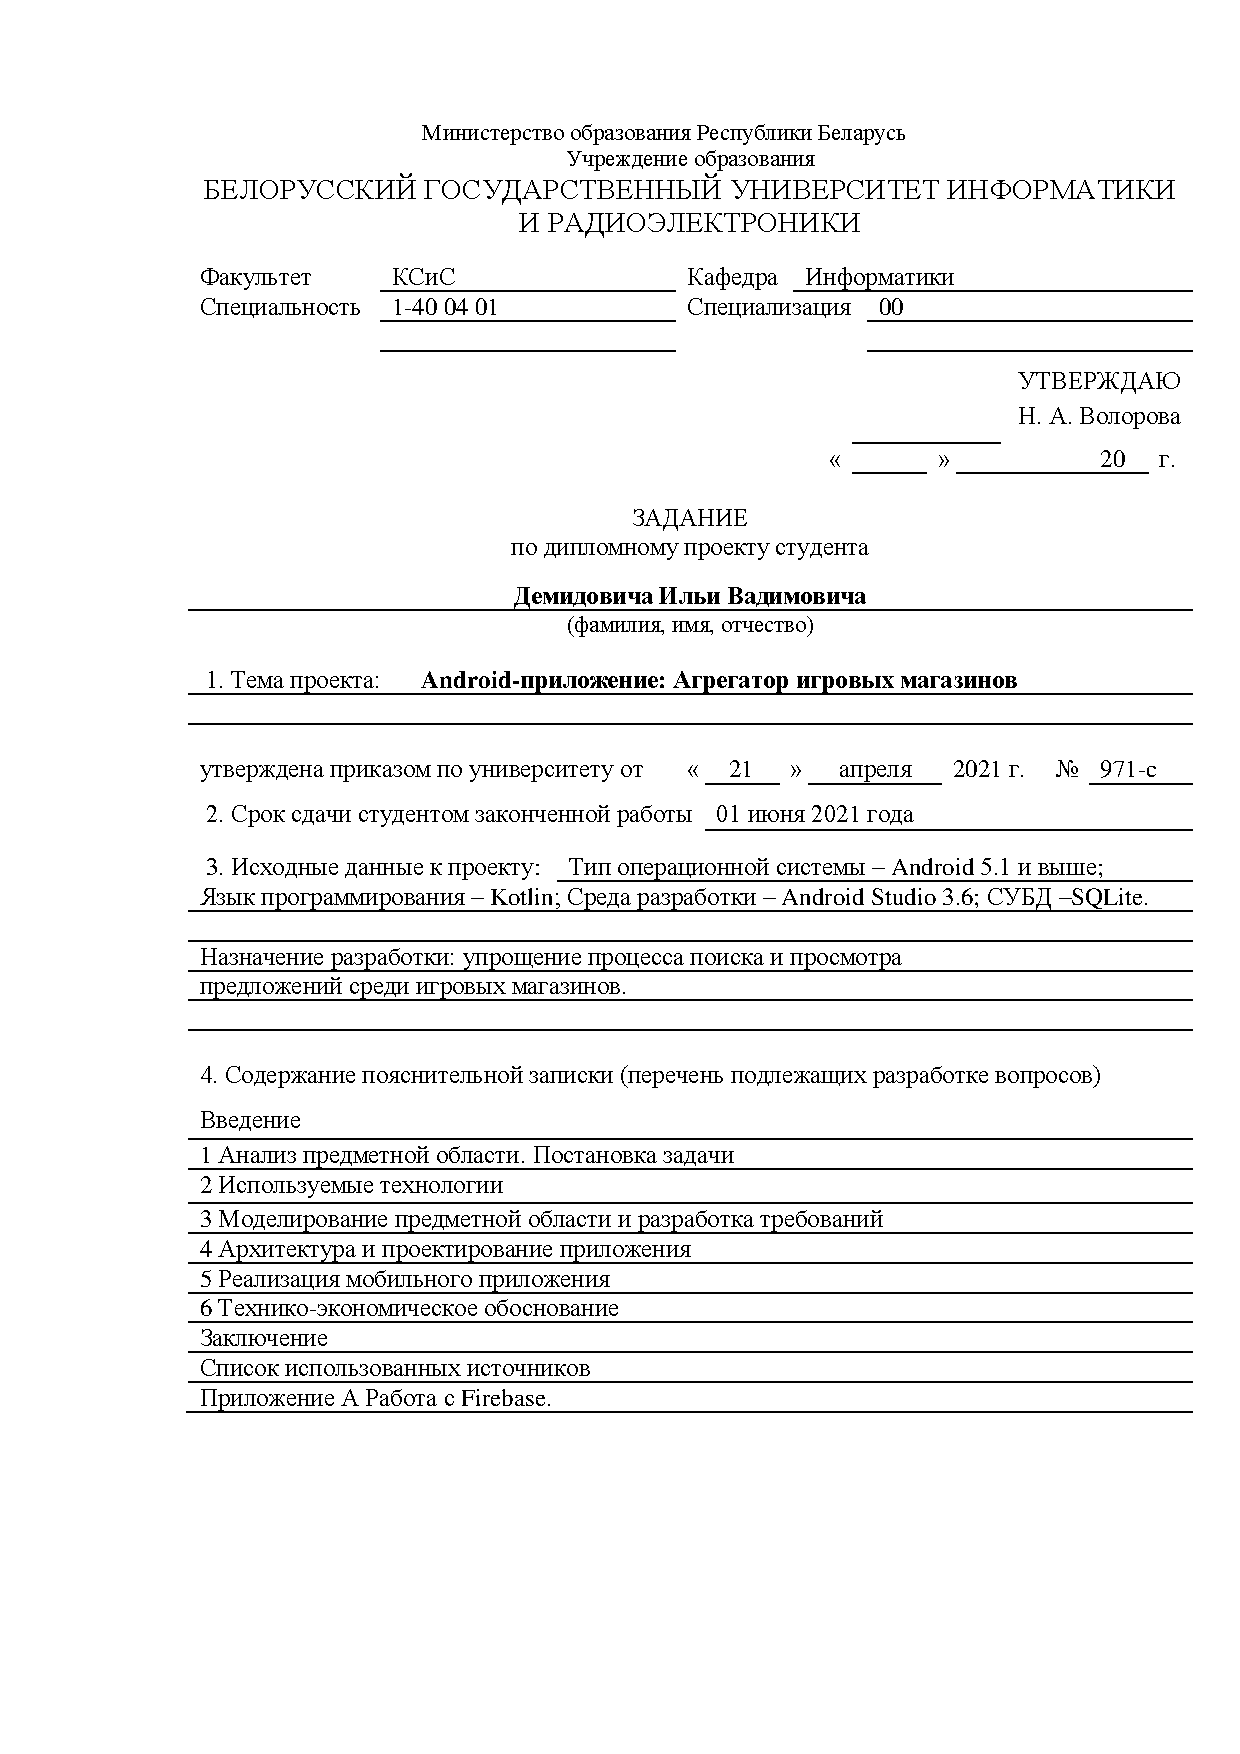
\includepdf[pages={1}]{task_1.pdf}
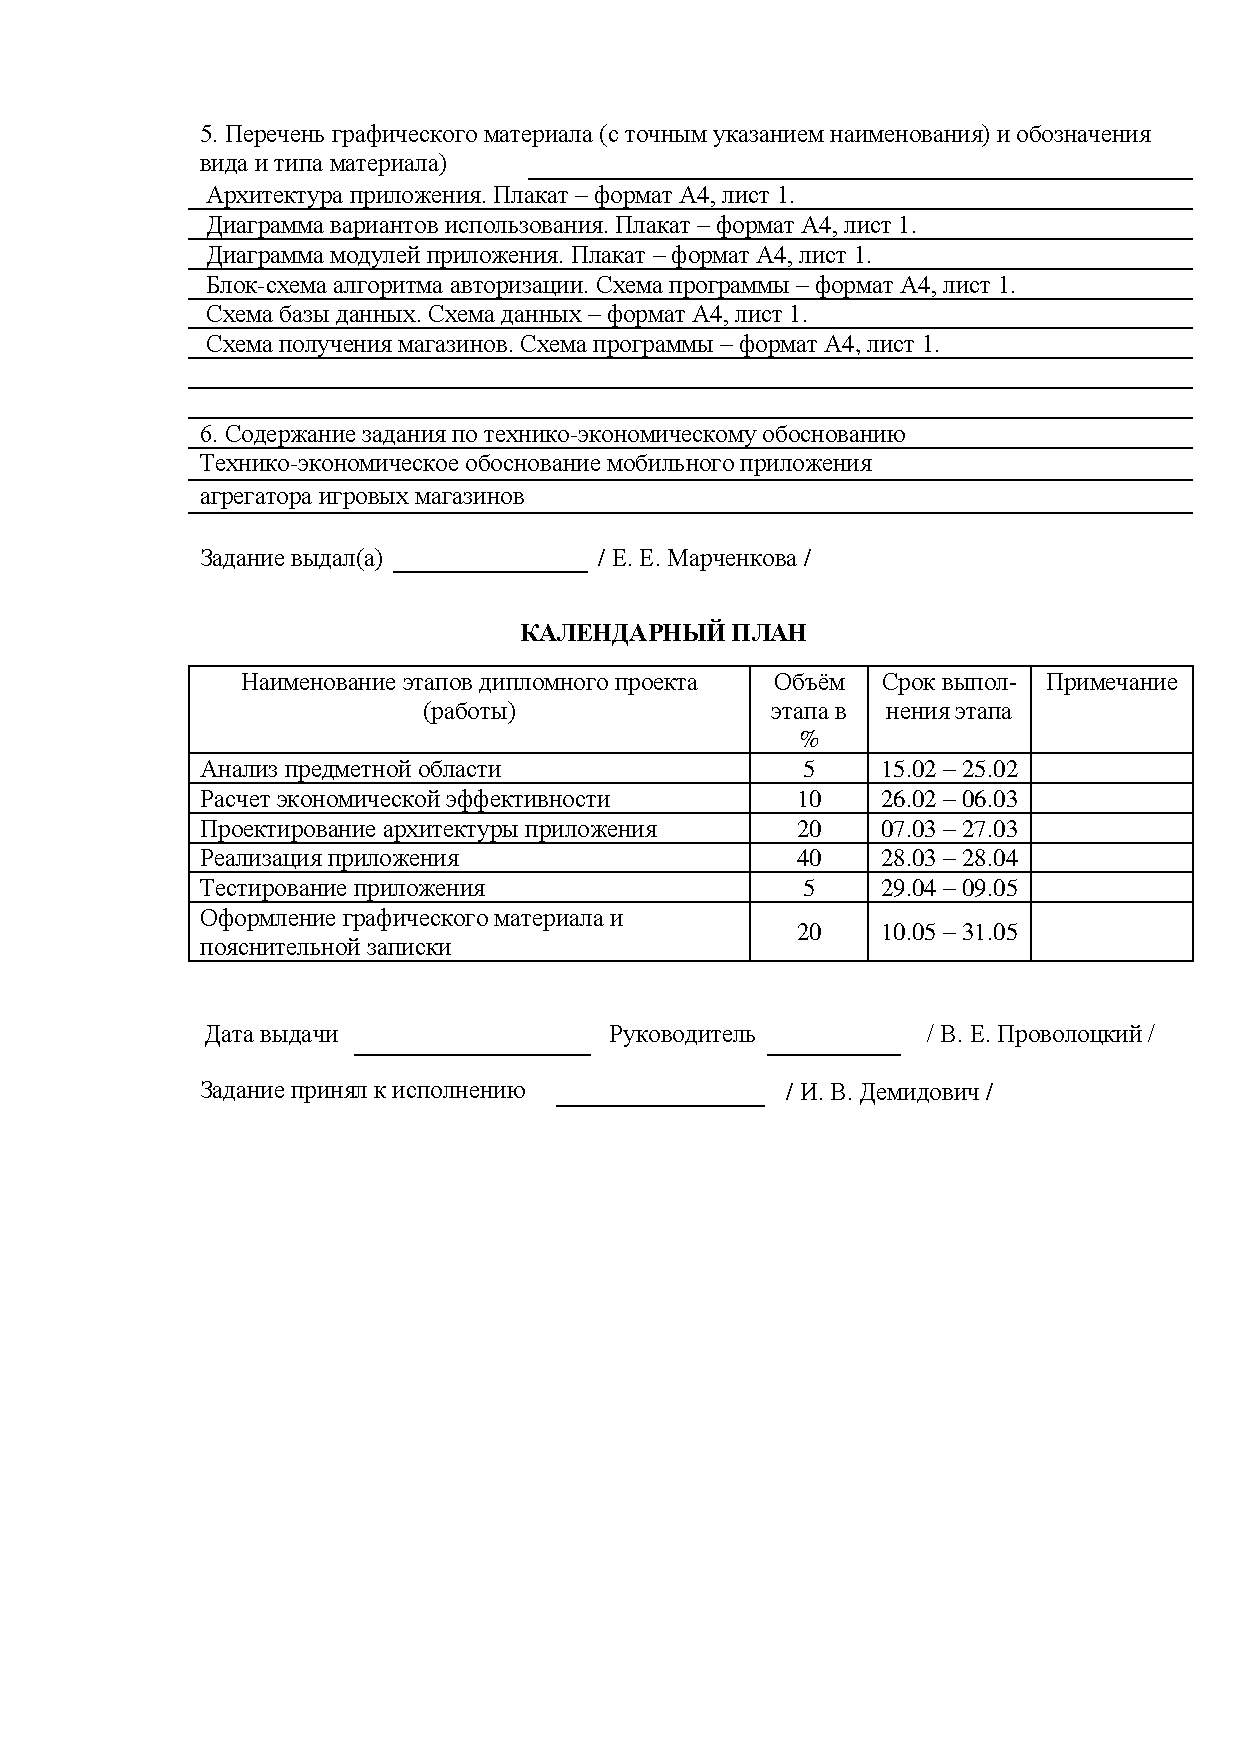
\includepdf[pages={1}]{task_2.pdf}

%{
  \newgeometry{top=1.25cm,bottom=1.25cm,right=1cm,left=2cm,twoside}
  \thispagestyle{empty}
  \setlength{\parindent}{0em}

  \newcommand{\lineunderscore}{\uline{\hspace*{\fill}}}

  \begin{center}
    Министерство образования Республики Беларусь\\
    Учреждение образования\\
    БЕЛОРУССКИЙ ГОСУДАРСТВЕННЫЙ УНИВЕРСИТЕТ \\
    ИНФОРМАТИКИ И РАДИОЭЛЕКТРОНИКИ\\[1em]
  

  \begin{minipage}{\textwidth}
    \begin{flushleft}
      \begin{tabular}{ l }
        Факультет: ФКСиС. Кафедра: Информатики. \\
        Специальность: 40 04 01 "Информатика и технологии программирования".
      \end{tabular}
    \end{flushleft}
  \end{minipage}\\[1em]

  \begin{minipage}{\textwidth}
    \begin{flushright}
      \begin{tabular}{p{0.40\textwidth}}
        УТВЕРЖДАЮ \\
        Заведующая кафедрой информатики \\
        \underline{\hspace*{7em}} Н. А. Волорова
        <<\underline{\hspace*{4ex}}>> \underline{\hspace*{5em}} 2020 г.
      \end{tabular}
    \end{flushright}
  \end{minipage}\\[1em]

  \text{ЗАДАНИЕ} \\
  \text{по дипломному проекту студента}

  {\text{Краcильникова Артём Андреевича}}

  \end{center}

  1. Тема проекта: \textquote{Онлайн кинотеатр}~--- утверждена приказом по университету от 21 апреля 2020 г.  \No{} 971-с

  \vspace{1em}

  2. Срок сдачи студентом законченного проекта: \underline{\hspace*{5em}}

  \vspace{1em}

  3. Исходные данные к проекту:\\
  % \uline{\hfill}\\
  % \uline{\hfill}\\
  % \uline{\hfill}\\
  % \uline{\hfill}\\
  % \uline{\hfill}\\
  \lineunderscore\\
  \lineunderscore\\
  \lineunderscore\\
  \lineunderscore\\
  \lineunderscore\\

  \vspace{1em}

  4. Содержание пояснительной записки (перечень подлежащих разработке вопросов):
  % \uline{\hfill}\\
  % \uline{\hfill}\\
  % \uline{\hfill}\\
  % \uline{\hfill}\\
  % \uline{\hfill}\\
  % \uline{\hfill}\\
  % \uline{\hfill}\\
  % \uline{\hfill}\\
  \lineunderscore\\
  \lineunderscore\\
  \lineunderscore\\
  \lineunderscore\\
  \lineunderscore\\
  \lineunderscore\\
  \lineunderscore\\
  \lineunderscore\\


  \clearpage
  \thispagestyle{empty}

  5. Перечень графического материала (с точным указанием обязательных чертежей):
  % \uline{\hfill}\\
  % \uline{\hfill}\\
  % \uline{\hfill}\\
  % \uline{\hfill}\\
  % \uline{\hfill}\\
  % \uline{\hfill}
  \lineunderscore\\
  \lineunderscore\\
  \lineunderscore\\
  \lineunderscore\\
  \lineunderscore\\
  \lineunderscore\\


  \vspace{1em}

  6. Содержание задания по технико-экономическому обоснованию:\\
  \uline{1. Описание функций, назначения и потенциальных пользователей ПО\hfill}\\
  \uline{2. Расчет затрат на разработку ПО\hfill}\\
  \uline{3. Экономический эффект при разработке ПО\hfill}
  \vspace{1em}

  ЗАДАНИЕ ВЫДАЛА \hfill{}  Т.\,А.~Рыковская  

  \vspace{1em}

  \vfill

  \begin{center}
    КАЛЕНДАРНЫЙ ПЛАН
  \end{center}

  \begin{tabular}{| >{\centering}m{0.04\textwidth} 
                  | >{\centering}m{0.40\textwidth} 
                  | >{\centering}m{0.08\textwidth}
                  | >{\centering}m{0.19\textwidth}  
                  | >{\centering\arraybackslash}m{0.16\textwidth}|}
    \hline \No{} п/п & Наименование этапов дипломного проекта & Объем этапа, \% & Срок выполнения этапов & Примечание \\
    \hline 1 & \raggedright Анализ предметной области, разработка технического задания & 15 & 24.03 - 30.03 & \\
    \hline 2 & \raggedright Разработка функциональных требований, проектирование архитектуры программы & 20 & 31.03 - 15.04 & \\
    \hline 3 & \raggedright Разработка схемы программы, алгоритмов, схемы данных & 15 & 16.04 - 20.04 & \\
    \hline 4 & \raggedright Разработка программного средства & 30 & 21.04 - 12.05 & \\
    \hline 5 & \raggedright Тестирование и отладка & 10 & 13.05 - 15.05 & \\
    \hline 6 & \raggedright Оформление пояснительной записки и графического материала & 20 & 18.05 - 1.06 & \\
    \hline
  \end{tabular}

  \vspace{2em}

  Дата выдачи задания: \underline{\hspace*{5em}} \\
  Руководитель \hfill{} М.\,В.~Стержанов

  \vspace{1em}

  ЗАДАНИЕ ПРИНЯЛ К ИСПОЛНЕНИЮ \hfill{} А.\,А.~Красильников

  \restoregeometry
} % pages 3 and 4. printed separately

%\sectioncentered*{Аннотация}
\thispagestyle{empty}

\begin{center}
  \begin{minipage}{0.82\textwidth}
    на дипломный проект <<Android-приложение: агрегатор игровых магазинов>> студента УО <<Белорусский государственный университет информатики и радиоэлектроники>> Демидовича~И.\,В.
  \end{minipage}
\end{center}

\emph{Ключевые слова}: приложение, мобильное, магазин, игры, предложение.
\vspace{1\parsep}

Целью дипломного проекта является разработка мобильного приложения, которое должно облегчить процесс поиска лучших предложений среди игровых магазинов на рынке.

Первый раздел содержит обзор предметной области, разбор аналогов создаваемого программного продукта. На основе проведенного анализа формулируются требования к проектируемому программному продукту.

В втором разделе производится обзор технологий, использованных для реализации программного продукта.

В третьем разделе проводится моделирование предметной области и разработка требований для программного продукта.

Четвертый раздел посвящен проектированию архитектуры приложения. В нём рассмотрены основные модули и компоненты, которые необходимо реализовать в программном продукте.

В пятом разделе дано описание процесса разработки программного продукта в рамках дипломного проекта, описания основных особенностей реализации, примеры использования и информация о тестировании.

В шестом разделе предоставлено технико-экономическое обоснование эффективности разработки программного продукта.

В заключении подводятся итоги проделанной работы и делаются выводы по дипломному проекту. Также описывается дальнейший план развития проекта.

Дипломный проект выполнен самостоятельно и проверен в системе «Антиплагиат». Цитирования обозначены ссылками на публикации, указанные в «Списке литературы».
\begin{figure}[H]
  \centering
    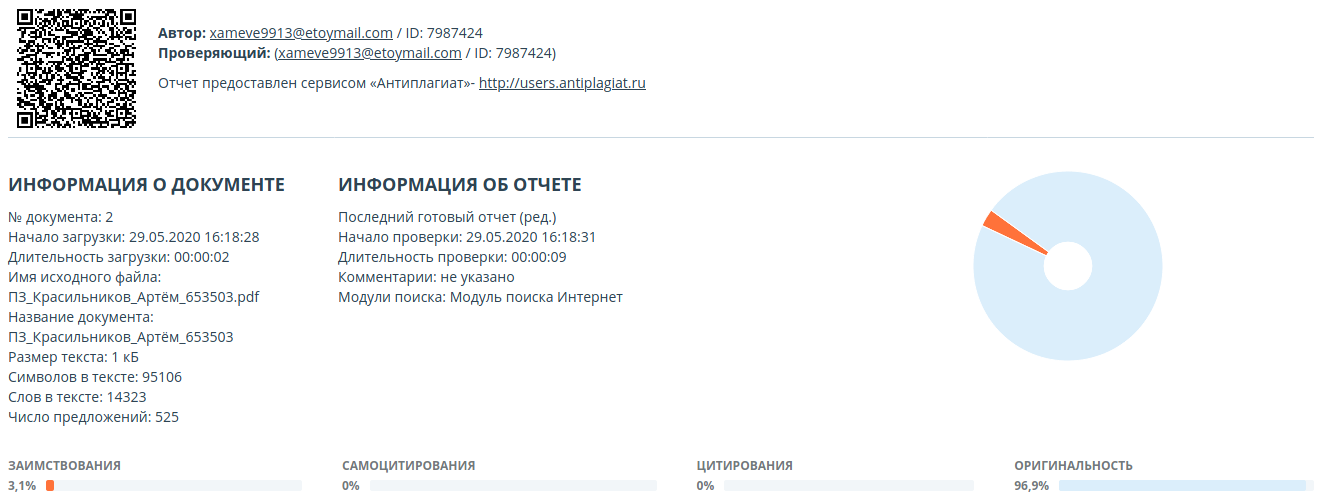
\includegraphics[scale=0.3]{anti.png} 
    \label{fig:anti}
 \end{figure}
\clearpage % not part of report

% % Содержимое данного документа позаимсвовано из Приложения Е из документа http://www.bsuir.by/m/12_113415_1_66883.pdf
 
\thispagestyle{empty}
 
\begin{singlespace}
 
{\small
 \begin{center}
   \begin{minipage}{0.8\textwidth}
     \begin{center}
       {\normalsize ОТЗЫВ}\\[1em]
       на дипломный проект студента факультета компьютерных систем и сетей Учреждения образования <<Белорусский государственный университет информатики и радиоэлектроники>>\\
       Красильников Артёма Андреевича \\
       на тему: <<Онлайн кинотеатр>>
     \end{center}
   \end{minipage}
 \end{center}
 
На время дипломного проектирования перед студентом Красильниковым~А.\,А. была поставлена задача разработать приложение видеоплеер для совместного просмотра видео на расстоянии.
Тема является актуальной, т.\,к. многие пользователи, не имеющие возможности собраться вместе со своими друзьями и знакомыми, нуждаются в дополнительных средствах социализации.
 
Красильников~А.\,А. на основании анализа аналогичных приложений и литературы, посвящённой передаче данных по сети, предложил проект веб-видеоплеера.
 
В процессе проектирования были разработаны структура данных, система синхронизации, модуль управления плеером.
Система разработана с использованием современных технологий и решений.
 
Работа над проектом велась в соответствии с календарным графиком.
Пояснительная записка и графический материал оформлены хорошо и в соответствии с требованиями ЕСКД.

В качестве замечаний можно выделить:
\begin{itemize}
  \item недостаточно подробное описание проектирования приложения;
  \item неполный формат описания вариантов использования (отсутствуют постусловия);
  \item наличие орфографических и синтаксических ошибок и опечаток.
\end{itemize}
 
Дипломный проект Красильникова~А.\,А. соответствует техническому заданию и выполнен с применением современных прогрессивных технологий. Рекомендуется оценка ‘семь’.
 
Считаю, что Красильников~А.\,А. освоил технику инженерного проектирования технических систем, подготовлена к самостоятельной работе по специальности 1-40~04~01
<<Информатика и технологии программирования>> и заслуживает присвоения квалификации инженера-системного программиста.
 
 \vfill
 \noindent
 \begin{minipage}{0.54\textwidth}
   \begin{flushleft}
     Руководитель проекта:\\
     канд. техн. наук, доцент,\\
     доцент кафедры информатики БГУИР\\
     1.06.20
   \end{flushleft}
 \end{minipage}
 \begin{minipage}{0.44\textwidth}
   \begin{flushright}
     \underline{\hspace*{3cm}} М.\,В.~Стержанов
   \end{flushright}
 \end{minipage}
}
 
\end{singlespace}
 
\clearpage
 

 % not part of report

%% Содержимое данного документа позаимсвовано из Приложения Ж из документа http://www.bsuir.by/m/12_113415_1_66883.pdf
 
\thispagestyle{empty}
 
\begin{singlespace}
 
{\small
 \begin{center}
   \begin{minipage}{0.9\textwidth}
     \begin{center}
       {\normalsize РЕЦЕНЗИЯ}\\[0.2cm]
       на дипломный проект студента факультета компьютерных систем и сетей Учреждения образования <<Белорусский государственный университет информатики и радиоэлектроники>>\\
       Красильникова Артём Андреевича \\
       на тему: <<Онлайн кинотеатр>>
     \end{center}
   \end{minipage}\\
 \end{center}
 
Дипломный проект студента Красильникова А. А. состоит из шести листов графического материала и~\pageref*{LastPage} страницы пояснительной записки.
 
Тема проекта является актуальной и посвящена разработке видеоплеера для совместного просмотра видео на расстоянии.
 
Пояснительная записка построена логично и последовательно отражает все этапы разработки в соответствии с календарным планом.
 
В пояснительной записке сделан обзор современных приложений и сервисов для совместного просмотра видео, разобраны способы синхронизации и необходимые технологии.
Разобраны способы синхронизации видео и технологии необходимые для этого.
Разобраны особенности технологий используемых для разработки и причины их выбора.
Программное обеспечение свидетельствуют о глубоких знаниях студента Красильникова~А.\,А. в области проектирования подобных систем, умении работать с технической литературой и применять на практике наиболее рациональные решения.
 
Пояснительная записка и графический материал оформлены аккуратно и в соответствии с требованиями ЕСКД.
 
Замечания:
\begin{itemize}
 \item описаны не все особенности реализации;
 \item имеются неоднозначные формулировки;
\end{itemize}
 
В целом дипломный проект выполнен удовлетворительно, в соответствии с техническим заданием на проектирование и заслуживает оценки шесть баллов, а диплом
ник Красильников~А.\,А. "--- присвоения квалификации инженера-системного программиста.
 
 \vfill
 \noindent
 \begin{minipage}{0.4\textwidth}
   \begin{flushleft}
     Рецензент:\\
     канд. техн. наук, доцент\\
     кафедры информатики БГУИР
   \end{flushleft}
 \end{minipage}
 \begin{minipage}{0.58\textwidth}
   \begin{flushright}
   \underline{\hspace*{3cm}}\hspace*{0.5cm}\underline{\hspace*{2cm}} М.\,В.~Стержанов \\
   Дата\hspace*{6.5cm}
   \end{flushright}
 \end{minipage}
}
 
\end{singlespace}
\clearpage

 % not part of report


% Зачем: Содержание пишется полужирным шрифтом, по центру всеми заглавными буквами
% Почему: Пункт 2.2.7 Требований по оформлению пояснительной записки.
\pagenumbering{gobble}
\renewcommand \contentsname {\centerline{\bfseries\large{\MakeUppercase{содержание}}}}

% Зачем: Не захламлять основной файл
% Примечание: \small\selectfont злостный хак, чтобы уменьшить размер шрифта в ToC 
{
\normalsize\selectfont
\tableofcontents
\newpage
}
\pagenumbering{arabic}


\sectioncentered*{ПЕРЕЧЕНЬ УСЛОВНЫХ ОБОЗНАЧЕНИЙ, СИМВОЛОВ И ТЕРМИНОВ}
\addcontentsline{toc}{section}{Перечень условных обозначений, символов и терминов}
\setcounter{page}{6}
\setlength{\parindent}{0ex}
В настоящей пояснительной записке применяются следующие определения и сокращения.

ПО~--- программное обеспечение.

ОС~--- операционная система.

UX~--- дизайн взаимодействия с пользователем.

UI~--- пользовательский интерфейс.

API~--- Application Programming Interfaces.

LLVM~--- Low Level Virtual Machine.

NDK~--- Native Development Kit.

JVM~--- Java Virtual Machine.

XML~--- eXtensible Markup Language.

СУБД~--- база данных.

SQL~--- structured query language~--- язык структурированных запросов.

NoSQL~--- not only SQL~--- не только SQL.

JSON~--- текстовый формат обмена данными,основанный на JavaScript.

HTTP~--- HyperText Transfer Protocol.

ПС~--- программное средство.

MVVM~--- Model View ViewModel.

ВИ~--- вариант использования.
\setlength{\parindent}{\fivecharsapprox}
\newpage


\sectioncentered*{Введение}
\addcontentsline{toc}{section}{Введение}
\label{sec:intro}

Темой дипломного проекта является «Android-приложение: Агрегатор игровых магазинов».

Развитие информационных технологий и игрового рынка изменяет процесс взаимодействия между пользователями и дистрибьюторами. С каждым годом появляется всё больше игровых магазинов, а их предложения начинают пересекаться, либо сильно разниться. 

Если обратиться к рейтингу посещаемости игровых магазинов по версии Alexa Traffic Rank \cite{web0} за 2021 год, можно заметить что пользователи интересуются всё большим количеством магазинов, как пример Epic Games Store ворвался на вторую строчку по траффику среди игровых магазинов всего за 2 года, что добавляет пользователям ещё больше выбора.
Востребованность игровой отрасли можно также объяснить эпидемией коронавируса, множество локдаунов и карантинов привели к изоляции большой части общества у себя дома, что вызывает большой рост игровой индустрии в целом и магазинов как её медиаторов.
Повышение количества магазинов также связывается с развитием индустрии в целом, еще в 90-ых годах было невозможно представить, что какая-то конкретная игровая студия откроет свой собственный сервис по продаже игр со своими скидами, бонусами и эксклюзивными предложениями.

Из-за глобальной пандемии COVID-19 и в следствии изоляции и отсутствия у большинства людей капитала как было раньше, образовался спрос на скидки, разные выгодные предложения, которые позволяют потреблять контент за сравнительно малые деньги, в следствии этого и возникла идея создать удобное мобильное приложение для отслеживания скидок и предложений по играм с разных игровых магазинов, а так же поиском этих самых предложений и игр.

%\section{Анализ предметной области. Постановка задачи}
\label{sec:domain}
 
В рамках данного раздела будет произведён обзор предметной области данного дипломного проекта.
Также будут рассмотрены возможные варианты реализаций и необходимые для этого технологий, сервисы, предлагающие аналогичные возможности, их плюсы и минусы и будут сформулированы основные требования к разрабатываемому ПО.
 
\subsection{Цель дипломного проекта}
Для определения ключевых функций приложения был произведён анализ статистики самых популярных и схожих по тематике приложений и сервисов. После изучения полученных результатов было решено, что необходимо создать современное приложение, которое совмещало бы в себе поиск приложений по популярным игровым магазинам, социальные функции, современный и простой интерфейс, который позволит пользователю в кратчайшие сроки найти себе приложение и магазин по душе.

\subsection{Формат разрабатываемого приложения}
В самом начале необходимо определиться с тем, как данное приложение будет функционировать. Под этим подразумевается необходимость выбора между разработкой настольного/мобильного или веб-приложения.
 
Под настольным приложением понимается программа, которую пользователь устанавливает на свой компьютер под управлением Windows/Linux, зачастую данные приложения требуют довольно долгой установки и зависимых библиотек уже установленных в системе \cite{web1}.

Говоря о мобильном приложении, имеется в виду установочный файл/архив, который пользователь скачивает с магазина приложений. Для таких приложений система не требует дополнительных установок библиотек и работает всегда, за исключением критических ситуаций.

Веб-приложение довольно популярный формат в 2021 году и набирает популярность, не требует ничего кроме браузера, за исключением ситуаций, когда требуется определённая версия браузера.

Рассмотрим плюсы и минусы этих реализаций ПО.

Для настольных приложений характерна высокая степень интеграции с системой пользователя и более низкое потребление системных ресурсов, однако они стремительно теряют свою популярность, так как мобильные и веб-приложения оказываются в более выгодной ситуации в плане установки, потребления и простоте. Если говорить о ходе разработки настольных приложениях, то оно сопровождается множеством платформенных зависимостей, которые зачастую пропускают специфичные для ОС функции.

Разработка веб-приложения, которое позже нужно будет адаптировать под мобильные платформы, чаще всего совпадает с потерей UX пользователя, как такового. При переносе сайтов в мобильную среду теряются нативные функции платформ, которые делают использование приложений более приятным для пользователя. Также это связано с потерей производительности и оптимизацией ПО.

Рынок мобильных приложений растёт с каждой секундой огромными темпами, поэтому самый популярный и самый эффективный метод это разработка мобильных приложений под какие-либо сервисы. Каждый год Google выпускает новые версии своих SDK с новыми возможностями улучшить жизнь пользователя, что на 2021 год даёт огромное пространство для реализаций своих идей. На текущий момент выбрана реализация мобильного приложения для Android среды.

\subsection{Анализ аналогов}

\undersection{Game Deals Tracker}~\par
Мобильное приложение от компании J\&C Studio, предоставляющий пользователям поиска игр по таким магазинам как Steam и Playstation Store. Game Deals Tracker обладает сравнительно небольшим функционалом: поиск, отображение скидок, вкладка «Рекомендуемые», возможность фильтровать результаты. Из важных для проекта возможностей стоит выделить, функцию просмотра скриншотов игр из Steam и Playstation Store, а также просмотром отзывов из этих магазнов. На рисунке~\ref{fig:domain:game_deals_tracker} можно видеть пример отображения информации об игре из Steam. Также хорошей функцией является вкладка «Исследовать» , которая является своеобразным дашбордом, в который пользователь может заходить без конкретной цели и искать себе игры по душе.
 
\begin{figure}[H]
 \centering
   
\includegraphics[scale=0.4]{game_deals_tracker.jpg} 
   \caption{Отдельная игра из Steam}
   \label{fig:domain:game_deals_tracker}
\end{figure}
 
Плюсы:
\begin{itemize}
 \item неплохой UI/UX;
 \item вкладка «Исследовать»;
 \item отображение отзывов и скриншотов из Steam;
 \item возможность синхронизировать настройки через единый аккаунт;
 \item поиск и его фильтры.
\end{itemize}
 
Минусы:
\begin{itemize}
 \item в основной части приложения всего два магазина для основного поиска и работы с его результатами;
 \item для вкладки с сохранением понравившихся предложений и игр пользователь обязан регистрироваться;
 \item реклама при переходах на отдельные экраны.
\end{itemize}
 
\undersection{Bargain Bytes - Game Deals}~\par
Game Deals от Rockspin, довольно популярное приложение, обладающие простым функционалом по поиску игр из разных магазинов. Главными функциями данного приложения является поиск по множеству магазинов, а также удобная вкладка WatchList, которая присылает нотификации в центр уведомлений телефона, когда цена упала до определённой отметки, что зачастую является очень удобной функцией для конечного пользователя. (пример на рисунке~\ref{fig:domain:game_deals_bytes}).
 
\begin{figure}[H]
 \centering
   
\includegraphics[scale=0.25]{game_deals_bytes.png} 
   \caption{Вкладка WatchList}
   \label{fig:domain:game_deals_bytes}
\end{figure}
 
Плюсы:
\begin{itemize}
 \item простой интерфейс;
 \item не требуется регистрация;
 \item множество магазинов.
\end{itemize}
 
Минусы:
\begin{itemize}
 \item устаревший UI/UX;
 \item приложение неоптимизированно;
 \item мало информации о конкретном предложении.
\end{itemize}

\undersection{CheapShark.com}~\par
CheapShark.com от AngrySoftware. Удобное настольное приложение для Windows, позволяет искать по разным магазинам и находить нужное приложение. Из отличительных функций нотификации на емейл по конкретному предложению, когда цена достигнет нужной отметки. Неплохим функционалом является просмотр игр от конкретного магазина. (пример на рисунке~\ref{fig:domain:game_cheap_shark}).

\begin{figure}[H]
  \centering
    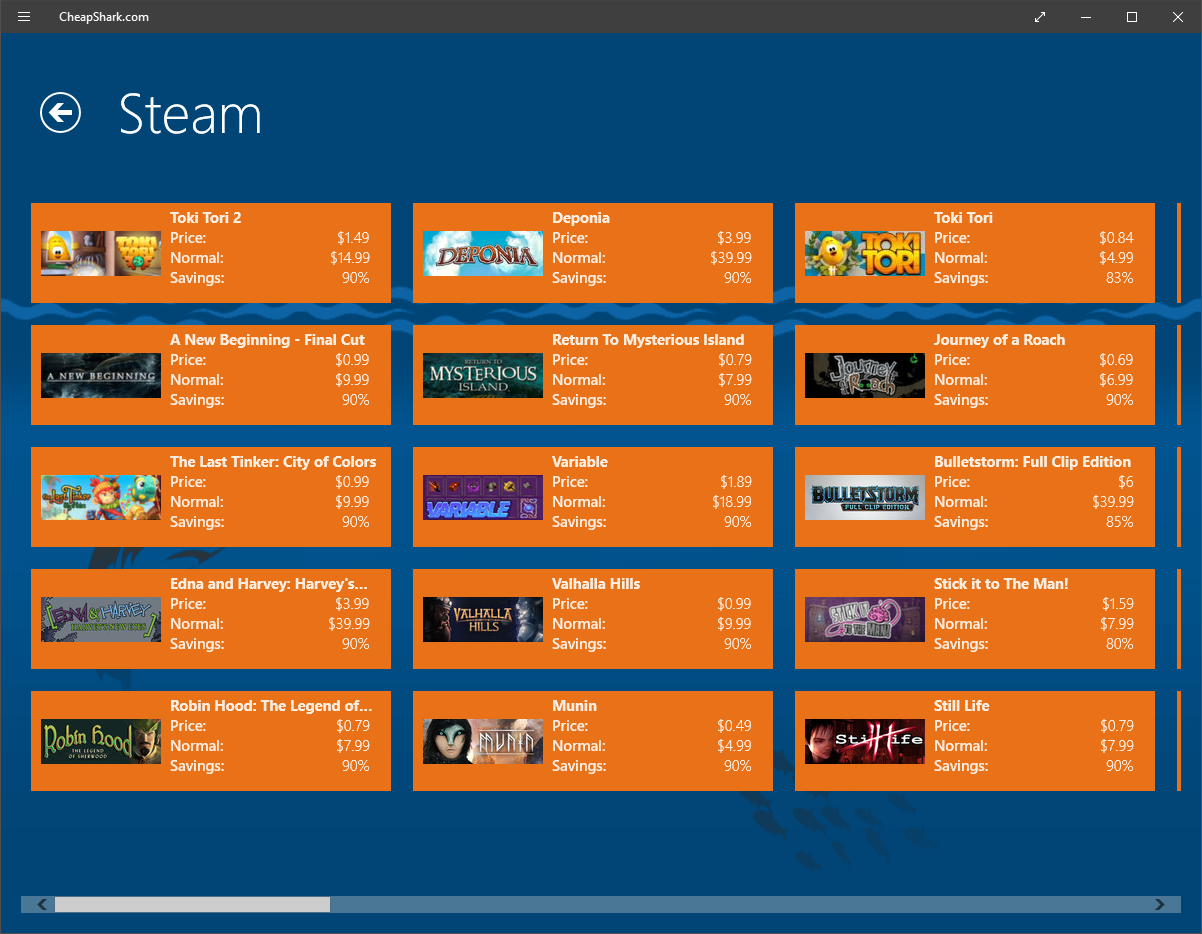
\includegraphics[scale=0.5]{game_deals_cheap_shark.png} 
    \caption{Приложение CheapShark}
    \label{fig:domain:game_cheap_shark}
 \end{figure}

Плюсы:
\begin{itemize}
  \item удобный настольный интерфейс;
  \item множество магазинов;
  \item просмотр игр по отдельному магазину;
  \item отсутствует реклама.
\end{itemize}

 Минусы:
 \begin{itemize}
  \item очень мало функционала;
  \item нет поиска;
  \item показаны не все игры от магазина;
  \item нет фильтров.
\end{itemize}
 
\subsection{Постановка задачи}
В рамках данного дипломного проекта необходимо разработать мобильное приложение агрегатор игровых магазинов. При разработке необходимо выполнить следующие задачи:
\begin{itemize}
 \item разработать приложение, которое будет агрегировать игровые магазины;
 \item разработать пользовательский интерфейс для приложения;
 \item реализовать поддержку сторонних ресурсов: Steam, Metacritic, и так далее.
\end{itemize}
 
\subsection{Требования к приложению}
Одним из самых важных этапов при разработке является сбор и организация требований. Хорошо описанные требования существенно снижают риски при проектировании архитектуры, разработке и тестировании программного продукта. Приложение не требует собственных внешних серверов, будут использованы несколько сторонних API сервисов по выдаче нужной информации о играх и их скидках. Приложение не требует сильных оптимизаций со стороны железа и кода, будет достаточно любого устройства работающего под Android 5-ой версии и выше. С железной части ПО, так же требованих никаких нет, на данный момент Play Store поддерживает формат Bundle, что представляет собой архив собранный под всевозможные процессоры существующие на рынке Android смартфонов. 
 
\undersection{Нефункциональные требования}
\begin{itemize}
 \item минимизировать затраты на разработку первой версии приложения;
 \item мобильное приложение должно работать на большом количестве мобильных устройств, минимальная версия Android SDK 23+;
 \item поддержка новейшего Android API;
 \item сопровождение более старых версий Android.
\end{itemize}
 
\undersection{Функциональные требования}
\begin{itemize}
  \item поддержка множества магазинов;
  \item возможность фильтровать ответы;
  \item вкладка избранное;
  \item вкладка исследование;
  \item возможность удобного поиска.
\end{itemize}
 
\subsection{Перспективы развития приложения}
В дальнейшем приложение может быть улучшено при помощи введения дополнительных возможностей:
\begin{itemize}
  \item подключение дополнительных функций для разных магазинов;
  \item собственная библиотека игр;
  \item инетграция прямых трансляций по определенной игре;
  \item расширение списка магазинов;
  \item добавление большего числа социальных функций.
\end{itemize}


%\section{Используемые технологии}
\label{sec:practice:technology_used}

\subsection{Выбор языка программирования}
Так как было решено решено разработать Android-приложение, разработку необходимо вести на языке, который имеет поддержку для выполнения в среде Android. К таковым можно отнести: Java, Kotlin, C++. Каждый из языков имеет место быть в Android разработке, рассмотрим каждый из них.

Java — самый популярный на данный момент язык для Android разработки. Большое коммьюнити, много библиотек и готовых модулей. Разработчик всегда может рассчитывать на быструю помощь по любому вопросу от коммьюнити, если он пишет на этом языке.

Плюсы:
\begin{itemize}
 \item большое сообщество готовое помочь;
 \item огромное количество учебных материалов;
 \item множество плагинов для сред разработки упрощяющих жизнь.
\end{itemize}

Минусы:
\begin{itemize}
 \item неоправданно громоздкий код;
 \item в следствии трендов для Android разработки, код на Java постепенно переходит в статус Legacy;
 \item новые библиотеки обходят Java стороной, в основном новые библиотеки пишут на Kotlin.
\end{itemize}
 
Kotlin — статически типизированный, объектно-ориентированный язык программирования, работающий поверх Java Virtual Machine и разрабатываемый компанией JetBrains. Также компилируется в JavaScript и в исполняемый код ряда платформ через инфраструктуру LLVM \cite{kotlin1}. С недавнего времени стал одним из предпочитаемых и официальных языков для р азработки под Android \cite{web2}.

Плюсы:
\begin{itemize}
 \item полностью совместим с Java;
 \item null safety. По умолчанию в Kotlin переменные не могут принимать null, если вы явно их так не обозначите;
 \item higher-Order Functions, т.е. функции которые принимают функции, как параметры;
 \item в перспективе лучший выбор для Android разработки.
\end{itemize}

Минусы:
\begin{itemize}
 \item зачастую не использует функциональность из старших версий JVM;
 \item присутствуют проблемы с annotation processing;
 \item всё ещё не все плагины для Java адаптированы для Kotlin;
 \item язык молодой, могут присутствовать баги.
\end{itemize}

С++ (Android NDK) — позволяет писать лишь некоторые части на C++ для обеспечения кроссплатформенности библиотек. Является инструментом для решения локальных проблем и не может рассматриваться как основной язык для написания Android приложений \cite{web12}.

Также рассмотрим другие альтернативы в виде Flutter и React Native, как самые популярные фрейморвки для разработки мобильных приложений.

Flutter — SDK с открытым исходным кодом для создания мобильных приложений от компании Google. Он используется для разработки приложений под Android и других платформ.

Плюсы:
\begin{itemize}
 \item кроссплатформенность;
 \item перспективность и активное развитие;
 \item важнейшие библиотеки уже есть, постоянно выходят новые;
 \item собственный графический движок;
 \item интерфейс легко разбивается на отдельные модули.
\end{itemize}

Минусы:
\begin{itemize}
 \item конечный установочный пакет больше, так как в него добавляется виртуальная машина Dart;
 \item интерфейс создается с помощью кода, из-за чего грань между логикой и дизайном гораздо тоньше;
 \item библиотек (и информации) меньше, чем для нативной разработки;
 \item нестабильность (совсем недавно вышел из beta).
\end{itemize}


React Native позволяет создавать мобильные приложения, используя при этом только JavaScript с такой же структурой, что и у React. Это дает возможность составлять многофункциональный мобильный UI с применением декларативных компонентов. Список плюсов и минусов совпадает с Flutter, за исключением собственного графического движка, React Native работает нативно на всех платформах используя их средства.

Фреймворки всегда являлись хорошим выбором для прототипирования за счёт быстроты, универсальности между платформами, однако имеют существенный минус в перспективе. В случае с Flutter - язык разработки Dart, а в случае с React Native - JavaScript/TypeScript. В конечном итоге у комнады будет 3 языка на которых они пишут для поддержки (по 1 нативному на каждоую мобильную платформу и 1 язык для фреймворка), что влечёт за собой не только баги, но и отсутствие или сложность имплементации сложного нативного функционала.

\subsection{Kotlin}
Таким образом был сделан выбор в сторону языка Kotlin. Он является относительно молодым и перспективным языком для Android разработки, который не устареет в ближайшее время и будет получать всё больше поддержки и библиотек. В случае Kotlin, который возник как язык на Java Virtual Machine или JVM, существует дополнительный уровень между компилятором и OS. Компилятор Kotlin создает так называемый байт-код, который запускается на JVM и попутно преобразуется в собственный код. Kotlin начал с JVM, но теперь можно скомпилировать Kotlin непосредственно в собственный код. Собственно это и создает ту самую полную совместимость с Java. Основным плюсом по отношению к Java является более простой код, рассмотрим несколько особенностей:

\begin{itemize}
 \item 1 — Язык позволяет, определяя переменные, поля, константы и тд, указать, может ли в них храниться ссылка на null. Поднимает на новый уровень идею аннотаций вроде @Nullable и NotNull, позволяет умно приводить к не-nullable типу после проверки её на null;
 \item 2 — Kotlin позволяет выводить тип переменной на основании данных, которыми переменная инициализируется. Поэтому при инициализации переменной тип можно опустить:;
 \item 3 — Bозможность, которой остро не хватает в Java для увеличения гибкости языка и решений. Заключается в возможности определить метод для типа отдельно от его (типа) объявления. Такая функция, конечно, не будет виртуальной и никак не меняет класса, которому мы добавляем метод, однако позволяет добавить как утилитарную функциональность для уже существующего кода, так и разгрузить интерфейс от этих же утилитарных методов. И у Kotlin функция — это сущность первого класса, если переводить дословно. Т.е. функции можно не только объявлять прямо в пакете (из Java они видны всё равно в классах — по имени файла), но и передавать в качестве параметров, возвращать из других функций и тд.
\end{itemize}
 
\subsection{Построение пользовательского интерфейса}
Далее встаёт вопрос визуализации пользовательского интерфейса. Интерфейс мобильного приложения на Android представляет собой набор XML файлов. 
XML, стили, векторные ресурсы определяют структуру и визуальное оформление содержимого мобильного приложения. Стандартный путь построения интерфейсов это XML файлы с его описанием, однако относительно недавно в бету вышел Jetpack Compose, что является новым словом в UI для Android. Рассмотрим оба варианта:

Jetpack Compose — это современный набор инструментов для создания собственного пользовательского интерфейса в Android-приложении. Этот декларативный фреймворк упрощает и ускоряет разработку пользовательского интерфейса на Android с меньшим количеством кода, мощными инструментами и интуитивно понятными API-интерфейсами Kotlin \cite{web13}.
 
Плюсы:
\begin{itemize}
 \item перспективность и активное развитие;
 \item переиспользование компонентов;
 \item более простая работа с редактором;
 \item пишутся на Kotlin.
\end{itemize}

Минусы:
\begin{itemize}
 \item сырая;
 \item маленькое комьюнити;
 \item библиотека всё еще в бета версии;
 \item тесная связь между отображением и бизнес-логикой.
\end{itemize}

XML — стандартный и стабильный вариант построения интерфейсов для приложений на Android, интерфейсы описываются в xml файлах, после этого обрабатываются во их фрагментах и активностях.

Плюсы:
\begin{itemize}
 \item стабильность;
 \item большое комьюнити;
 \item версии библиотек стабильные;
 \item разделение между представлением и бизнес-логикой.
\end{itemize}

Минусы:
\begin{itemize}
 \item низкая переиспользуемость.
\end{itemize}

Для проекта выберем XML, так как Jetpack Compose при всех его минусах, всё ещё очень сырая, а для перспективы нам нужна более стабильная система интерфейсов.

\subsection{Синхронизация данных}
При разработке мобильного приложения необходимо определиться c технологиями и подходом к методам синхронизации и обмена данными, а также стратегией кэширования, которые доступны для реализации в мобильном приложении. Были рассмотрены следующие варианты: ленивый кеш, синхронизированный кеш и кеш сквозной записи. 
 
В проекте будет реализована локальная SQL (в частности SQLite) база данных для кеширования, серверная NoSQL база данных для сохранения настроек пользователя, а также запросы на сторонние сервисы через интернет.

SQLite — компактная встраиваемая СУБД. Слово «встраиваемый» означает, что SQLite не использует парадигму клиент-сервер, то есть движок SQLite не является отдельно работающим процессом, с которым взаимодействует программа, а представляет собой библиотеку, с которой программа компонуется, и движок становится составной частью программы \cite{sqlite1}. Таким образом, в качестве протокола обмена используются вызовы функций (API) библиотеки SQLite. Такой подход уменьшает накладные расходы, время отклика и упрощает программу. SQLite хранит всю базу данных (включая определения, таблицы, индексы и данные) в единственном стандартном файле на том устройстве, на котором исполняется программа. Простота реализации достигается за счёт того, что перед началом исполнения транзакции записи весь файл, хранящий базу данных, блокируется; ACID-функции достигаются в том числе за счёт создания файла журнала.

Несколько процессов или потоков могут одновременно без каких-либо проблем читать данные из одной базы. Запись в базу можно осуществить только в том случае, если никаких других запросов в данный момент не обслуживается; в противном случае попытка записи оканчивается неудачей, и в программу возвращается код ошибки. Другим вариантом развития событий является автоматическое повторение попыток записи в течение заданного интервала времени.

Для того, чтобы упростить разработку приложения, было решено использовать сервис Firebase от компании Google. Данный сервис предлагает множество модулей, которые очень полезны для мобильной разработки. Данный сервис избавляет от нужды в собственном сервере, так как Firebase реализует практически все возможности, которые необходимы от стандартного сервера. Главным инструментом в составе Firebase является их база данных. На данный момент Firebase предлагает несколько различных вариантов баз данных: Realtime Database и Firestore. Их главное отличие заключается в форме хранения данных и доступа к ним. 

Realtime Database использует JSON файлы для хранения информации. Это является крайне неэффективным, так как для получения определённых данных сначала нужно получить все данные из файла, а только потом можно произвести поиск. Это увеличивает потребность приложения в ресурсах системы, что недопустимо для данного проекта. 

Firestore~--- облачная NoSQL база данных реального времени. Это означает то, что, при использовании данной базы данных, пользователь может «подписаться» на определённые документы. В таком случае при изменении содержимого документа пользователь сразу получит новые данные. Благодаря данному механизму можно быть уверенным, что конечный пользователь получит самую свежую информацию. Firestore поддерживает следующие типы данных:

\begin{itemize}
    \item текстовая строка;
    \item числа;
    \item булевые значения;
    \item массивы;
    \item даты;
    \item словари.
\end{itemize}

Для удалённой базы данных будем использовать Firebase/Firestore как дефакто стандарт для Android приложений. Так как Firestore является NoSQL базой данных, то для организации данных в ней используются не таблицы, а документы. Отличие заключается в том, что документ не имеет жёсткой структуры, как таблицы, что позволяет хранить в документах данные произвольных типов и менять их значение и структуру по мере необходимости. Данный способ позволяет более гибко взаимодействовать с данными, но лишает дополнительной надёжности, свойственной SQL базам данных.

Для организации документов используются коллекции. Коллекция~--- это просто набор документов. Они не обязаны быть одинаковыми, но данный случай крайне нежелателен. Каждый документы в коллекции имеет идентификатор, уникальный для данной коллекции. В качестве идентификатора может выступать любая подходящая текстовая строка. Документы также способны содержать внутри себя вложенные коллекции, однако данная возможность не особо полезна. Также имеется возможность создания пользовательских функций и триггеров для взаимодействия с базой данных, что позволяет выполнять определённые операции при изменении, создании или удалении документов и коллекций. 

Firebase также предлагает встроенную систему аутентификации пользователей, которая поддерживает различные источники для идентификации: почта, профиль Google и др.

Также плюсом Firebase является возможность его интеграции с другими сервисами компании Google и дополнительная защита от прекращения работы собственного сервера.

\subsection{Недостатки Firebase}
Основные возможности, которые предоставляет Firebase связанные с хранением, изменением и получением информации из встроенной базы данных. Firebase не имеет возможности для создания API, поэтому для решения вспомогательных задач, не связанных с базой данных необходим дополнительный API-cервер, который будет заниматься обработкой запросов и обращаться к Firestore по мере необходимости.

Теперь рассмотрим стратегии локального кеширования:

Ленивый кеш — самый простой вид кеширования, но его нужно использовать осторожно, так как отдает устаревшие данные. Можно при каждой записи сбрасывать ленивый кеш, чтобы поддерживать актуальность данных, но тогда затраты на реализацию будут сравнимы с более сложными типами кеширования \cite{web15}.

Такой тип кеширования можно использовать для данных, которые почти никогда не меняются. Другой вариант использования – делать ленивый кеш с небольшим временем устаревания для стабильной работы при всплесках нагрузки.

Такой тип кеширования позволит быстрее всех дать ответ.

Синхронизированный кеш — самый полезный тип кеширования, так как отдает свежие данные и позволяет реализовать многоуровневый кеш.

Такой тип кеширования встроен в протокол HTTP. Сервер отдает метку изменения, а клиент кеширует у тебя результат и в последующем запросе передает эту метку. Сервер может дать ответ, что состояние не изменилось и можно использовать кешированный на клиенте объект. Сервер в свою очередь, получив метку может переспросить у хранилища были ли изменения или нет.

Этот тип кеширования не избавляет от накладных расходов на общение между системами. Поэтому часто дополняется другими типами кеширования, чтобы ускорить работу.

Кеш сквозной записи — если есть система распределенного кеширования (memcached, Windows Sever App Fabric, Azure Cache), то можно использовать кеш сквозной записи. Рукопашная реализация синхронизации кешей между узлами сама по себе отдельный большой проект, потому не стоит заниматься ей в рамках разработки приложения.

Не стоит пытаться кешировать все в синхронизированном кеше, иначе большая часть кода приложения будет заниматься перестройкой кеша.

Также не стоит забывать что системы распределенного кеширования также требуют общения между системами, что может сказываться на быстродействии.

В приложении будет использоваться ленивый кеш для данных, так как приложение является remote-first, то кеш данных нужен только для того, чтобы приложение функционировало без интернета, хоть и без части функциональности. Для картинок будет использоваться синхронизированный кеш, который реализуется в основном библиотеками.

% \section{Архитектура и проектирование приложения}
\label{sec:arch_and_mod}
 
\subsection{Android}
Так как для разработки был выбран Android SDK, то при разработке было решено придерживаться характерных для данной платформы архитектурных подходов.
На данный момент стандартом в Android разработке является MVVM.
Она заключается в отделении пользовательского интерфейса от логики приложения. Опишем каждый компонент данного архитектурного подхода. (cхема на рисунке~\ref{fig:arch:docs_connections}).

Model — слой с основной логикой программы.
View — пользовательский интерфейс.
ViewModel — связывающая прослойка между View и Model.

\begin{figure}[H]
 \centering
   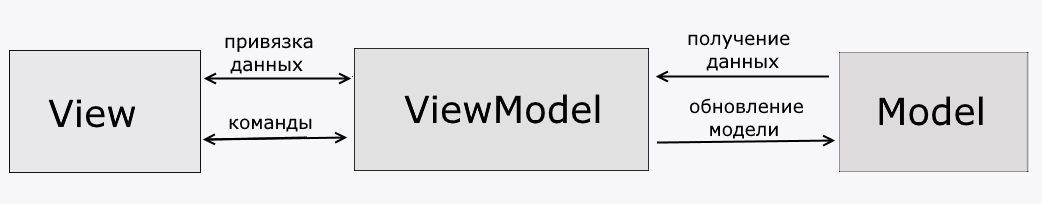
\includegraphics[scale=0.3]{mvvm.png} 
   \caption{MVVM}
   \label{fig:arch:docs_connections}
\end{figure}

Для упрощения реализации данной парадигмы проектирования и упрощения разработки, компания Google выпустила Android Architecture Components. Данный набор решений включает в себя:

\begin{itemize}
 \item Lifecycle - отслеживает текущий статус Activity и может уведомлять об этом своих подписчиков;
 \item LiveData - получает и хранит данные, может отправлять их своим подписчикам;
 \item ViewModel - поможет сохранить живыми необходимые для вас объекты при повороте экрана;
 \item Paging Library - библиотека для постраничной загрузки данных из базы данных, с сервера или любого другого источника;
 \item Navigation Architecture Component - новый компонент для навигации по экранам приложения;
 \item Work Manager - удобный механизм выполнения фоновых задач;
 \item Room - обёртка для работы с базой данных;
 \item Data Binding - избавление от рутины по написанию кода работающего со View.
 \end{itemize}

 Основные плюсы MVVM включают в себя:

\begin{itemize}
  \item лёгкость в тестировании (связи между логикой приложения и пользовательским интерфейсом ослабевает, что даёт большую гибкость в тестировании отдельных компонентов);
  \item прост в поддержке (высокая модульность и прозрачность слоёв архитектуры приносят простоту в отслеживании ошибок и расширении приложения);
  \item прозрачная комьюникация (ViewModel предоставляют простой интерфейс, который View использует для заполнения себя, сама же ViewModel связывает View с частью бизнес-логики приложения).
\end{itemize}
 
\subsection{Serverless архитектура}
Serverless-вычисления (бессерверные-вычисления) - модель облачных вычислений, в которых платформа динамически руководит выделением вычислительных ресурсов. 
В данном случае бессерверный не означает отсутствие сервера как такового, под этим понимается то, что пользователю конкретной платформы не нужно заниматься созданием и настройкой собственного сервера. 
Данный подход позволяет значительно сэкономить ресурсы и уменьшить срок разработки, так как многие важные аспекты серверной части на себе берёт платформа. 
В рамках данного проекта такой платформой выступает Firebase.
 
\subsection{Организация и описание модулей приложения}
Разработанное мобильное приложение можно разделить на три составляющие:
\begin{itemize}
 \item Клиентское приложения на Kotlin;
 \item Модуль Firebase для работы с базой данных;
 \item API cервер для получения данных;
\end{itemize}
 
Клиентское приложение является основным модулем для данного проекта. В рамках клиентского приложения реализованы основные функциональные возможности данного проекта:
\begin{itemize}
  \item поддержка множества магазинов;
  \item возможность фильтровать поиск по множеству фильтров;
  \item вкладка избранное, возможность добавлять игры или предложения в избранное;
  \item вкладка исследование, главная вкладка с предложениями которые ранжирует само приложение;
  \item просмотр дополнительной информации (рейтинг, самая высокая стоимость, самая низкая стоимость и тд);
  \item возможность перехода на сторонние магазины для покупки товара;
  \item социальные функции (шейринг, отображение графики, ведение статистики пользователя).
\end{itemize}
 
Модуль Firebase отвечает за авторизацию, управление данными пользователя, их организацию и процесс передачи данных клиентскому приложению.
 
API сервер представлет собой несколько сторонних бесплатных API серверов с базами данных игр и игровых магазинов. Основная функция этих серверов заключается в выдаче клиенту необходимой для работы информации (список магазинов, дополнительная информация об игре, поиск лучший предложений), а так же объединении нескольких сторонних API в единое целое на клиентской части.
 
На рисунке~\ref{fig:arch:modules_scheme} изображена схема взаимодействия вышеперечисленных модулей.
 
\begin{figure}[H]
 \centering
   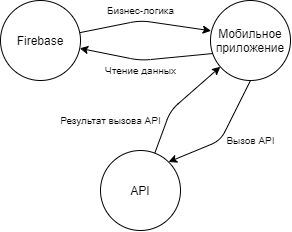
\includegraphics[scale=0.8]{api.png} 
   \caption{Структура модулей приложения}
   \label{fig:arch:modules_scheme}
\end{figure}
 
\section{Реализация мобильного приложения}
\label{sec:code}
По итогу разработки было реализовано мобильное приложение, которое позволяет пользователю находить лучшие предложения по продаже игр среди игровых магазинов.

\subsection{Базовые компоненты}

Для удобной и расширяемой архитектуры приложения были написаны базовые компоненты для Activity, Fragment, ViewModel. Рассмотрим каждый в отдельности.

\subsubsection{BaseActivity}~\par
Activity представляет собой отдельный модуль приложения с которым пользователь может взаимодействовать. Для удобства был написан базовый класс (см. листинг~\ref{lst:baseActivity}), который реализует обработку ошибок путем вызова диалогового окна с текстом ошибки, а так же показом прогресса загрузки данных с сервера дополнительно с блокированием интерфейса пользователя, пока запрос на сервер не будет выполнен. Помимо блокирования пользовательского интерфейса данная реализация решает проблему синхронизации при нескольких запросах на сервер путем @Synchronized аннотаций и проверок на существования прогресса на экране. Аннотация @Synchronized позволяет быть уверенным в том, что в данный метод заходит только 1 поток, при том, что для остальных потоков данный метод не будет доступен, пока первый поток не завершит свои задачи. Данный класс является базовым для любой Activity в приложении.

\begin{lstlisting}[language=Java,label={lst:baseActivity},caption={Компонент BaseActivity}]

abstract class BaseActivity<T : BaseViewModel> : BaseActivity() {
    protected abstract val viewModel: T

    private lateinit var progressDialog: ProgressDialog

    private lateinit var errorDialog: MaterialDialog

    override fun onCreate(savedInstanceState: Bundle?) {
        super.onCreate(savedInstanceState)
        setUpDialogs()
        observeUiChanges()
    }

    private fun setUpDialogs() {
        progressDialog = ProgressDialog()
        errorDialog = MaterialDialog(this).apply {
            positiveButton(text = "Ok")
        }
    }

    private fun observeUiChanges() {
        viewModel.apply {
            progress.observe(
                this@BaseActivity,
                { progress ->
                    handleProgress(progress = progress)
                }
            )

            errorEvent.observe(
                this@BaseActivity,
                { error ->
                    handleAhriError(ahriError = error)
                }
            )
        }
    }

    @Synchronized
    fun handleProgress(
        fragmentManager: FragmentManager = supportFragmentManager,
        progress: Boolean
    ) {
        if (progress) {
            if (!progressDialog.isAdded) {
                progressDialog.show(fragmentManager, ProgressDialog::class.java.canonicalName)
                fragmentManager.executePendingTransactions()
            }
        } else {
            if (progressDialog.isAdded) {
                progressDialog.dismissAllowingStateLoss()
                fragmentManager.executePendingTransactions()
            }
        }
    }

    @Synchronized
    fun handleAhriError(
        fragmentManager: FragmentManager = supportFragmentManager,
        ahriError: AhriError
    ) {
        handleError(fragmentManager, ahriError, ahriError.retryAction)
    }

    private fun handleError(
        fragmentManager: FragmentManager = supportFragmentManager,
        error: AhriError,
        retryAction: (() -> Unit)?
    ) {
        errorDialog.show {
            message(text = error.exception.message)
        }
    }
}
\end{lstlisting}

\subsubsection{BaseFragment}~\par
Fragment является модульной переиспользуемой частью Activity. Класс BaseFragment (см. листинг~\ref{lst:baseFragment}) является базовым классом для всех фрагментов в приложении. Данный класс реализует передачу событий загрузки в Activity, а так же логику по работе с клавиатурой и проверке доступов к различным подсистемам Android. Так же данный класс обязывает реализовывать для каждого фрагмента базовую ViewModel.

\begin{lstlisting}[language=Java,label={lst:baseFragment},caption={Компонент BaseFragment}]
abstract class BaseFragment<T : BaseViewModel> : BaseFragment() {
    protected abstract val viewModel: T

    override fun onActivityCreated(savedInstanceState: Bundle?) {
        super.onActivityCreated(savedInstanceState)
        observeUiEvents()
    }

    override fun onDestroyView() {
        hideKeyboard()
        requireActivity().currentFocus?.hideKeyboard()
        super.onDestroyView()
    }

    private fun observeUiEvents() {
        viewModel.apply {
            progress.observe(
                viewLifecycleOwner,
                { progress ->
                    (activity as BaseActivity<*>).handleProgress(
                        fragmentManager = childFragmentManager,
                        progress = progress
                    )
                }
            )

            errorEvent.observe(
                viewLifecycleOwner,
                { error ->
                    (activity as BaseActivity<*>).handleAhriError(
                        fragmentManager = childFragmentManager,
                        ahriError = error
                    )
                }
            )
        }
    }

    fun checkPermission(permission: String, requestPermissionCode: Int): Boolean {
        return if (ContextCompat.checkSelfPermission(requireContext(), permission) != PackageManager.PERMISSION_GRANTED) {
            if (shouldShowRequestPermissionRationale(permission)) {
                requestPermissions(arrayOf(permission), requestPermissionCode)
            } else {
                requestPermissions(arrayOf(permission), requestPermissionCode)
            }

            false
        } else {
            true
        }
    }

    protected fun openGoToSettingPermissionDialog(activityResultLauncher: ActivityResultLauncher<Intent>) {
        MaterialDialog(requireContext()).apply {
            title(res = R.string.base_dialog_title_runtime_permission_is_denied)
            message(text = getString(R.string.base_dialog_text_go_to_application_settings))
            cancelable(false)
            positiveButton(
                res = R.string.action_go_to_settings,
                click = {
                    val intent = Intent(ACTION_APPLICATION_DETAILS_SETTINGS)
                    val uri = Uri.fromParts("package", requireContext().packageName, null)
                    intent.data = uri
                    activityResultLauncher.launch(intent)
                }
            )
            negativeButton(res = R.string.action_cancel, click = { /* Nothing */ })
        }.show()
    }
}
\end{lstlisting}

\subsubsection{BaseViewModel}~\par
ViewModel — модель представления, которая служит прослойкой между View и Model. Такое разделение позволяет ускорить разработку и поддерживаемость программы — можно менять один компонент, не затрагивая код другого. Данная реализация базовой ViewModel (см. листинг~\ref{lst:baseViewModel}) включает в себя определение событий ошибок, загрузок, а так же вспомогательных методов для запросов в сеть.

\begin{lstlisting}[language=Java,label={lst:baseViewModel},caption={Компонент BaseViewModel}]
open class BaseViewModel : ViewModel(), CoroutineScope {

    val progress: MutableLiveData<Boolean> = MutableLiveData()

    override val coroutineContext = SupervisorJob() + Dispatchers.Main

    val errorEvent: LiveEvent<AhriError> = LiveEvent()

    suspend fun handleLoading(
        scope: CoroutineScope = viewModelScope,
        progress: MutableLiveData<Boolean> = this@BaseViewModel.progress,
        actionUseCase: Any? = null,
        block: suspend () -> Unit,
    ) {
        handleLoading(
            progress = progress,
            block = block,
            retryAction = {
                scope.launch {
                    handleLoading(scope, progress, actionUseCase, block)
                }
            }
        )
    }

    private suspend fun handleLoading(
        progress: MutableLiveData<Boolean> = this@BaseViewModel.progress,
        block: suspend () -> Unit,
        retryAction: () -> Unit
    ) {
        handleErrors(
            block = {
                try {
                    progress.value = true
                    block()
                } finally {
                    progress.value = false
                }
            },
            retryAction = retryAction
        )
    }

    suspend fun handleErrors(
        scope: CoroutineScope = viewModelScope,
        block: suspend () -> Unit,
    ) {
        handleErrors(
            block = block,
            retryAction = {
                scope.launch {
                    handleErrors(scope, block)
                }
            }
        )
    }

    private suspend fun handleErrors(
        block: suspend () -> Unit,
        retryAction: () -> Unit
    ) {
        try {
            block()
        } catch (ex: Throwable) {
            errorEvent.value = AhriError(ex, retryAction)

            Timber.tag("debug").e(ex.message ?: "")
        }
    }
}
\end{lstlisting}

\subsection{Слой данных и логики}
Всю бизнес-логику и логику работы с получением данных можно представить в виде дерева зависимостей, состоящего из:

\begin{itemize}
  \item слой Api для запросов на сервера;
  \item слой Database для работы с локальной базой данных;
  \item слой DataSource для получения данных либо из Api, либо из Database;
  \item слой Gateway для преобразования данных в модели приемлимые для приложения;
  \item слой UseCase для инкапсулирования логики Gateway и другой бизнес-логики.
\end{itemize}

На рисунке~\ref{fig:arch:data_diagram} изображена схема взаимодействия вышеперечисленных модулей.
 
\begin{figure}[H]
 \centering
   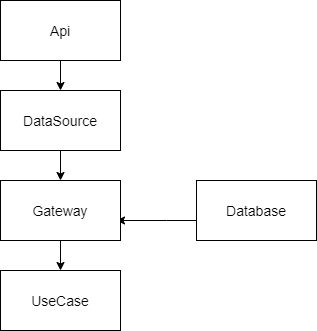
\includegraphics[scale=0.8]{data_diagram.png} 
   \caption{Структура слоя данных}
   \label{fig:arch:data_diagram}
\end{figure}
 
В качестве примера рассмотрим получение списка магазинов в приложении. Первым делом пользовательский интерфейс вызывает UseCase GetStores(см. листинг~\ref{lst:getStores}) их получения.

\begin{lstlisting}[language=Java,label={lst:getStores},caption={UseCase GetStores}]
class GetStores(private val storesGateway: StoresGateway) {
    suspend operator fun invoke(): List<Store> {
        return storesGateway.getStores()
    }
}
\end{lstlisting}

Данный UseCase вызывает StoresGateway (см. листинг~\ref{lst:storesGateway}), который осуществляет получение магазинов либо из базы данных, либо с сервера, попутно сохраняя их в базу данных. Данный метод проверяет наличие интернет подключение на устройстве, после этого делает запрос на сервер, либо в локальную базу данных, в зависимости от результата. Так же выполняются преобразования моделей в модели подходящие приложению. Если интернет подключение на устройстве присутствует и получение списка магазинов с сервера произошло успешно, то метод сохраняет полученные магазины в локальную базу данных для дальнейшего использования.
\begin{lstlisting}[language=Java,label={lst:storesGateway},caption={StoresGateway}]
class StoresGatewayImpl(
    private val storesDataSource: StoresDataSource,
    private val storesDao: StoreLocalDao,
    private val networkService: NetworkService
) : StoresGateway {
    override suspend fun getStores(cachedFirst: Boolean): List<Store> {
        val stores = storesDao.getStores()
        if ((cachedFirst && stores.count() > 0) || !networkService.isNetworkEnabled) {
            return storesDao.getStores().map { it.toDomain() }
        } else if (networkService.isNetworkEnabled) {
            val storesRemote = storesDataSource.getStores().map {
                Store(
                    it.storeID, it.storeName, it.isActive != 0,
                    StoreImage(
                        Uri.parse("${Constants.HOST_URL}${it.storeImage.bannerPath}"),
                        Uri.parse("${Constants.HOST_URL}${it.storeImage.logoPath}"),
                        Uri.parse("${Constants.HOST_URL}${it.storeImage.iconPath}")
                    )
                )
            }
            val storesDB = storesDao.getStores()
            storesRemote.forEach { storeItem ->
                val store = storesDB.findLast { item -> item.storeID == storeItem.id }
                if (store != null) {
                    storeItem.isSelected = store.isSelected
                }
            }
            storesDao.replaceStores(storesRemote.map { obj -> obj.toDb() })
            return storesRemote
        }
        return arrayListOf()
    }

    override suspend fun saveStores(stores: List<Store>) {
        storesDao.replaceStores(stores.map { obj -> obj.toDb() })
    }
}

\end{lstlisting}


StoresGateway применяет один из двух источников данных. При наличии подключения к интернету вызывается StoresDataSource(см. листинг~\ref{lst:storesDataSource}), который делает запрос на сервер.

\begin{lstlisting}[language=Java,label={lst:storesDataSource},caption={StoresDataSource}]
class StoresDataSource(private val api: Api) {
    suspend fun getStores(): List<StoreRemote> {
        return api.getStores()
    }
}
\end{lstlisting}

Интерфейс Api(см. листинг~\ref{lst:storesApi}) реализуется с помощью библиотеки Retrofit, которая является одной из самых популярных и удобных библиотек для запросов на сервер на устройствах Android.

\begin{lstlisting}[language=Java,label={lst:storesApi},caption={Api}]
interface Api {
    @GET("stores")
    suspend fun getStores(): List<StoreRemote>
}
\end{lstlisting}

Если же интернет подключение отсутствует, то вызывается StoresLocalDao (см. листинг~\ref{lst:storesLocalDao}), которое инкапсулирует логику для работы с локальной базой данных.
\begin{lstlisting}[language=Java,label={lst:storesLocalDao},caption={StoresLocalDao}]
@Dao
abstract class StoreLocalDao : BaseDao<StoreLocal> {
    @Query("SELECT * FROM stores")
    abstract suspend fun getStores(): List<StoreLocal>

    @Query("DELETE FROM stores")
    abstract suspend fun clearStores()

    @Transaction
    open suspend fun replaceStores(objects: List<StoreLocal>) {
        clearStores()
        insert(objects)
    }
}
\end{lstlisting}

\subsection{Внедрение зависимостей}
Внедрение зависимости — процесс предоставления внешней зависимости программному компоненту. Является специфичной формой инверсии управления, когда она применяется к управлению зависимостями. В полном соответствии с принципом единственной обязанности объект отдаёт заботу о построении требуемых ему зависимостей внешнему, специально предназначенному для этого общему механизму. Для внедрения зависимостей в работе используется легковесная библиотека Koin. Концепция области в Koin аналогична таковой в Android. Она позволяет, например, ограничить область живучести модели представления (ViewModel) до определенной активности и использовать эту модель во фрагментах, которыми наполняется активность. Как правило, в Koin три вида временных областей.

\begin{itemize}
  \item single, создается объект, который сохраняется в течение всего периода существования контейнера;
  \item factory, каждый раз создается новый объект, без сохранения в контейнере;
  \item scoped, создается объект, который сохраняется в рамках периода существования связанной временной области.
\end{itemize}

Для определения зависимостей в приложении используются следующие модули:
\begin{itemize}
  \item модуль Main, который определяет общие для всего приложения зависимости, как Api, базу данных, парсеры;
  \item модуль Database определяет источники данных для доступа к базе данных;
  \item модуль Service определяет вспомогательные сервисы для приложения;
  \item модуль DataSource определяет источники данных;
  \item модуль Gateway;
  \item модуль UseCase;
  \item модуль ViewModel.
\end{itemize}


В качестве примера приведён модуль Gateway (см. листинг~\ref{lst:gatewayModule}), определяющий все классы Gateway в приложении.
\begin{lstlisting}[language=Java,label={lst:gatewayModule},caption={GatewayModule}]
var gatewayModule = module {
    single<PreferencesGateway> {
        PreferencesGatewayImpl(preferenceDataSource = get())
    }
    single<StoresGateway> {
        StoresGatewayImpl(
            storesDataSource = get(),
            networkService = get(),
            storesDao = get()
        )
    }
    single<DealsGateway> {
        DealsGatewayImpl(
            dealsDataSource = get(),
            storesGateway = get(),
            favoriteDao = get(),
            dealDao = get()
        )
    }
    single<GamesGateway> {
        GamesGatewayImpl(
            gamesDataSource = get(),
            networkService = get(),
            storesGateway = get(),
            favoriteGameDao = get(),
            gameDao = get()
        )
    }
    single<AuthGateway> {
        AuthGatewayImpl()
    }
    single<StoriesGateway> {
        StoriesGatewayImpl()
    }
    single<BannersGateway> {
        BannersGatewayImpl()
    }
    single<RssGateway> {
        RssGatewayImpl(rssApi = get())
    }
}
\end{lstlisting}

\subsection{Манифест приложения}
Файл манифеста AndroidManifest.xml (см. листинг~\ref{lst:manifest}) предоставляет основную информацию о программе системе. Каждое приложение должно иметь свой файл AndroidManifest.xml. Файл манифеста инкапсулирует всю архитектуру Android-приложения, его функциональные возможности и конфигурацию. Корневым элементом манифеста является <manifest>. Помимо данного элемента обязательными элементами является теги <application> и <uses-sdk>. Элемент <application> является основным элементом манифеста и содержит множество дочерних элементов, определяющих структуру и работу приложения. Порядок расположения элементов, находящихся на одном уровне, произвольный. Все значения устанавливаются через атрибуты элементов. Кроме обязательных элементов, упомянутых выше, в манифесте по мере необходимости используются другие элементы.

\begin{lstlisting}[language=Xml,label={lst:manifest},caption={AndroidManifest.xml}]
<?xml version="1.0" encoding="utf-8"?>
<manifest xmlns:android="http://schemas.android.com/apk/res/android"
        package="com.lust.ahri">

    <uses-permission android:name="android.permission.ACCESS_NETWORK_STATE" />
    <uses-permission android:name="android.permission.READ_PHONE_STATE" />
    <uses-permission android:name="android.permission.INTERNET" />
    <uses-permission android:name="android.permission.CAMERA"/>
    <uses-permission android:name="android.permission.READ_EXTERNAL_STORAGE" />
    <uses-permission android:name="android.permission.WRITE_EXTERNAL_STORAGE" />

    <application
            android:name=".App"
            android:allowBackup="true"
            android:icon="@mipmap/ic_launcher"
            android:label="@string/app_name"
            android:roundIcon="@mipmap/ic_launcher_round"
            android:supportsRtl="true"
            android:theme="@style/AppTheme">

        <activity
                android:name="com.lust.ahri.view.main.MainActivity"
                android:label="@string/app_name"
                android:screenOrientation="portrait" />

        <activity
                android:name=".view.auth.AuthActivity"
                android:screenOrientation="portrait" />

        <activity
                android:name=".view.onboarding.OnboardingActivity"
                android:screenOrientation="portrait">
            <intent-filter>
                <action android:name="android.intent.action.MAIN" />
                <category android:name="android.intent.category.LAUNCHER" />
            </intent-filter>
        </activity>

        <service
                android:name=".core.service.firebase.AhriMessagingService">
            <intent-filter>
                <action android:name="com.google.firebase.MESSAGING_EVENT"/>
            </intent-filter>
        </service>

        <provider
                android:name="br.com.mauker.materialsearchview.db.HistoryProvider"
                android:authorities="br.com.mauker.materialsearchview.searchhistorydatabase"
                android:exported="false"
                android:protectionLevel="signature"
                android:syncable="true"/>

        <provider
                android:name="androidx.core.content.FileProvider"
                android:authorities="${applicationId}.fileprovider"
                android:exported="false"
                android:grantUriPermissions="true">
            <meta-data
                    android:name="android.support.FILE_PROVIDER_PATHS"
                    android:resource="@xml/file_paths" />
        </provider>

    </application>

</manifest>
\end{lstlisting}

\subsubsection{AhriMessagingService}~\par

Сервис который используется для получения и отображения нотификаций полученных через Firebase Cloud Messaging. Конкретной реализации данный сервис не имеет (см. листинг~\ref{lst:firebase_notifications}) и инкапсулирует базовую логику отображения нотификаций пользователю когда приложение выключено.

\begin{lstlisting}[language=Java,label={lst:firebase_notifications},caption={AhriMessagingService}]
class AhriMessagingService: FirebaseMessagingService() {

    override fun onMessageReceived(p0: RemoteMessage) {
        super.onMessageReceived(p0)
    }

    override fun onNewToken(p0: String) {
        super.onNewToken(p0)
    }
}
\end{lstlisting}

\subsubsection{HistoryProvider}~\par
Поставщик содержимого - это оболочка, в которую заключены данные. Если приложение использует базу данных SQLite, то только приложение имеет к ней доступ. Но бывают ситуации, когда данные желательно сделать общими. Простой пример - контакты из телефонной книги тоже содержатся в базе данных, но приложению нужно иметь доступ к данным, чтобы приложение тоже могло выводить список контактов. Так как исходное приложение не имеет доступа к базе данных чужого приложения, был придуман специальный механизм, позволяющий делиться своими данными всем желающим.

Данный поставщик содержимого не имеет конкретной реализации и используется для сохранения поисковых запросов пользователя. Данный поставщик включает в себя функционал удаления, добавления и обновления поисковых запросов.

\subsubsection{FileProvider}~\par
FileProvider является поставщиком содержимого который используется для доступа ко внутренним файлам приложения во время того как пользователь меняет свой аватар. Пример использования приведён ниже (см. листинг~\ref{lst:file_provider}).

\begin{lstlisting}[language=Java,label={lst:file_provider},caption={Использование FileProvider}]
    private fun getOutputMediaFile(name: String): Uri {
        val directory = requireActivity().applicationContext.getExternalFilesDir(null)
            ?: requireActivity().applicationContext.filesDir
        !directory.exists() && directory.mkdirs()

        return FileProvider.getUriForFile(
            requireActivity(),
            requireActivity().applicationContext.packageName + ".fileprovider",
            File(directory.path, name)
        )
    }
\end{lstlisting}

\subsection{Основные модули}

Приложение состоит из 7 взаимосвязанных модулей. Пользователь начинает знакомство с приложением с модуля приветствия после переходя в модуль авторизации, где ему будет необходимо зарегистрироваться в системе, после данных действий пользователь сможет взаимодействовать с основными модулями:

\begin{itemize}
  \item модуль исследования;
  \item модуль избранного;
  \item модуль поиска;
  \item модуль магазинов;
  \item модуль аккаунта.
\end{itemize}

\subsubsection{Модуль приветствия}~\par
Данный модуль создан для описания пользователю основных функций приложения. Модуль состоит из одной OnboardingActivity, которая в себя включает постраничное отображение преимуществ приложения. Пользователь может пропустить часть приветствия нажав кнопку SKIP и подтвердив свой выбор в диалоге. Пример пользовательского интерфейса представлен на рисунке~\ref{fig:arch:onboarding_1}.

\begin{figure}[H]
 \centering
   
\includegraphics[scale=0.8]{onboarding_1.png} 
   \caption{Модуль приветствия}
   \label{fig:arch:onboarding_1}
\end{figure}

Программная реализация включает OnboardingFragmentStateAdapter, который использует отдельный Fragment для каждой из страниц описания (см. листинг~\ref{lst:onboarding_code}). При постраничном перелистывании данный адаптер вызывает отдельный Fragment с описанием конкретной функции используя позицию для обозначения нужного фрагмента.


\begin{lstlisting}[language=Java,label={lst:onboarding_code},caption={OnboardingFragmentStateAdapter}]
class OnboardingFragmentStateAdapter(activity: FragmentActivity) : FragmentStateAdapter(activity) {

    override fun getItemCount(): Int = OnboardingStep.values().size

    override fun createFragment(position: Int): Fragment {
        return when (position) {
            OnboardingStep.STEP_1.ordinal -> OnboardingStep1Fragment()
            OnboardingStep.STEP_2.ordinal -> OnboardingStep2Fragment()
            OnboardingStep.STEP_3.ordinal -> OnboardingStep3Fragment()
            else -> {
                throw Exception("Wrong Implementation")
            }
        }
    }
}
\end{lstlisting}


При долистывании до конца или подтверждения пропуска приветствия приложение вызывает функцию launchMain (см. листинг~\ref{lst:launch_main}), которая проверяет аутентифицирован ли пользователь. В заввисимости от результата пользователь попадает на модуль авторизации, либо в главную часть приложения.

\begin{lstlisting}[language=Java,label={lst:launch_main},caption={Функция launchMain}]
    private fun launchMain() {
        viewModel.isOnboardingEnabled = false
        val intent = if (isLoggedIn()) {
            Intent(applicationContext, MainActivity::class.java)
        } else {
            Intent(applicationContext, AuthActivity::class.java)
        }
        startActivity(intent)
        finish()
    }
\end{lstlisting}


\subsubsection{Модуль авторизации}~\par

Модуль авторизации состоит из одной AuthActivity, а также нескольких фрагментов между которыми происходит навигация внутри этой Activity.

AuthStartFragment является стартовым фрагментом в AuthActivity, он позволяет совершить навигацию на фрагмент логина AuthSignInFragment или на фрагмент регистрации пользователя AuthSignUpFragment. Пример пользовательского интерфейса представлен на рисунке~\ref{fig:arch:auth_1}.

\begin{figure}[H]
 \centering
   
\includegraphics[scale=0.8]{auth_1.png} 
   \caption{Стартовый фрагмент модуля авторизации}
   \label{fig:arch:auth_1}
\end{figure}

AuthSignInFragment выполняет функцию аутентификации пользователя с помощью емейла и пароля, так же имея возможность перейти на экран восстановления пароля AuthResetPasswordStep1Fragment или на экран регистрации пользователя AuthSignUpFragment. Пример пользовательского интерфейса представлен на рисунке~\ref{fig:arch:auth_2}.

\begin{figure}[H]
 \centering
   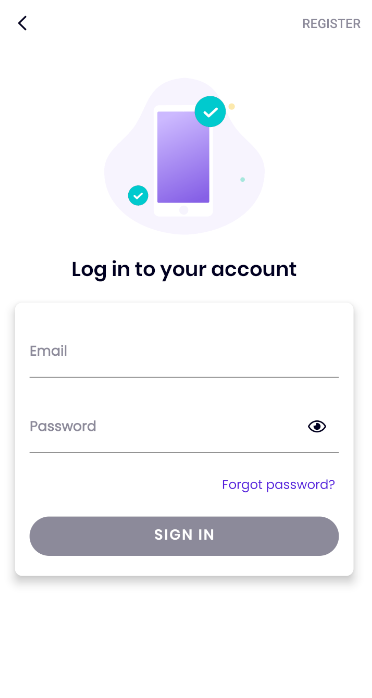
\includegraphics[scale=0.8]{auth_2.png} 
   \caption{Фрагмент аутентификации пользователя}
   \label{fig:arch:auth_2}
\end{figure}

Программная реализация содержит AuthSignInViewModel, который проводит базовую валидацию полей емейла и пароля с помощью ValidateEmail и ValidatePassword (см. листинг~\ref{lst:auth_sign_in_vm}).

\begin{lstlisting}[language=Java,label={lst:auth_sign_in_vm},caption={AuthSignInViewModel}]
class AuthSignInViewModel(
    private val validateEmail: ValidateEmail,
    private val validatePassword: ValidatePassword,
    private val signIn: SignIn
) : BaseViewModel() {
    val password: MutableLiveData<String> = MutableLiveData()
    val email: MutableLiveData<String> = MutableLiveData()

    private val _initSignInEvent: LiveEvent<Nothing> = LiveEvent()
    val initSignInEvent: LiveData<Nothing>
        get() = _initSignInEvent

    private val _openResetPasswordEvent: LiveEvent<Nothing> = LiveEvent()
    val openResetPasswordEvent: LiveData<Nothing>
        get() = _openResetPasswordEvent

    val isSignUpDataValid: LiveData<Boolean> = combineLatest(email, password) {
        val email = email.value
        val password = password.value

        if (email != null && password != null) {
            return@combineLatest email.isNotEmpty() && password.isNotEmpty()
        }

        return@combineLatest false
    }

    private val _passwordValidationEvent: LiveEvent<ValidatePassword.Result> =
        LiveEvent()
    val passwordValidationEvent: LiveData<ValidatePassword.Result>
        get() = _passwordValidationEvent

    private val _emailValidationEvent: LiveEvent<ValidateEmail.Result> =
        LiveEvent()
    val emailValidationEvent: LiveData<ValidateEmail.Result>
        get() = _emailValidationEvent

    private fun validatePassword(): Boolean {
        val result = validatePassword(password.value)
        _passwordValidationEvent.emit(result)
        return when (result) {
            ValidatePassword.Result.Valid -> true
            ValidatePassword.Result.NotValid, ValidatePassword.Result.IsEmpty -> false
        }
    }

    private fun validateEmail(): Boolean {
        val result = validateEmail(email.value)
        _emailValidationEvent.emit(result)
        return when (result) {
            ValidateEmail.Result.Valid -> true
            ValidateEmail.Result.IsEmpty, ValidateEmail.Result.NotValid -> false
        }
    }

    private fun validateSignInInputs(): Boolean {
        return validatePassword() && validateEmail()
    }

    fun forgotPassword() {
        _openResetPasswordEvent.emit()
    }

    fun logIn() {
        validateSignInInputs().applyIfTrue {
            viewModelScope.launch {
                handleLoading {
                    signIn(email.value!!, password.value!!)
                    _initSignInEvent.emit()
                }
            }
        }
    }
}
\end{lstlisting}

При нажатии на кнопку Sign In клиентское приложение делает запрос на Firebase Auth с помощью logIn метода (см. листинг~\ref{lst:auth_sign_in_uc}), который проверяет правильность введенных данных и делает запрос на сервер с этими данными. При неправильно введенных данных пользователь получает оповещение в виде сообщения на экране, что нужно ввести правильные данные.

\begin{lstlisting}[language=Java,label={lst:auth_sign_in_uc},caption={SignIn}]
    override suspend fun signIn(email: String, password: String) {
        return suspendCoroutine { cont ->
            auth.signInWithEmailAndPassword(email, password)
                .addOnCompleteListener {
                    if (it.isSuccessful) {
                        cont.resume(Unit)
                    } else {
                        cont.resumeWithException(Exception("Wrong login or password"))
                    }
                }
        }
    }
\end{lstlisting}

AuthSignUpFragment производит регистрацию пользователя с помощью емейла, пароля и имени пользователя, так же имея возможность перейти на AuthSignInFragment. Пример пользовательского интерфейса представлен на рисунке~\ref{fig:arch:auth_3}.

\begin{figure}[H]
 \centering
   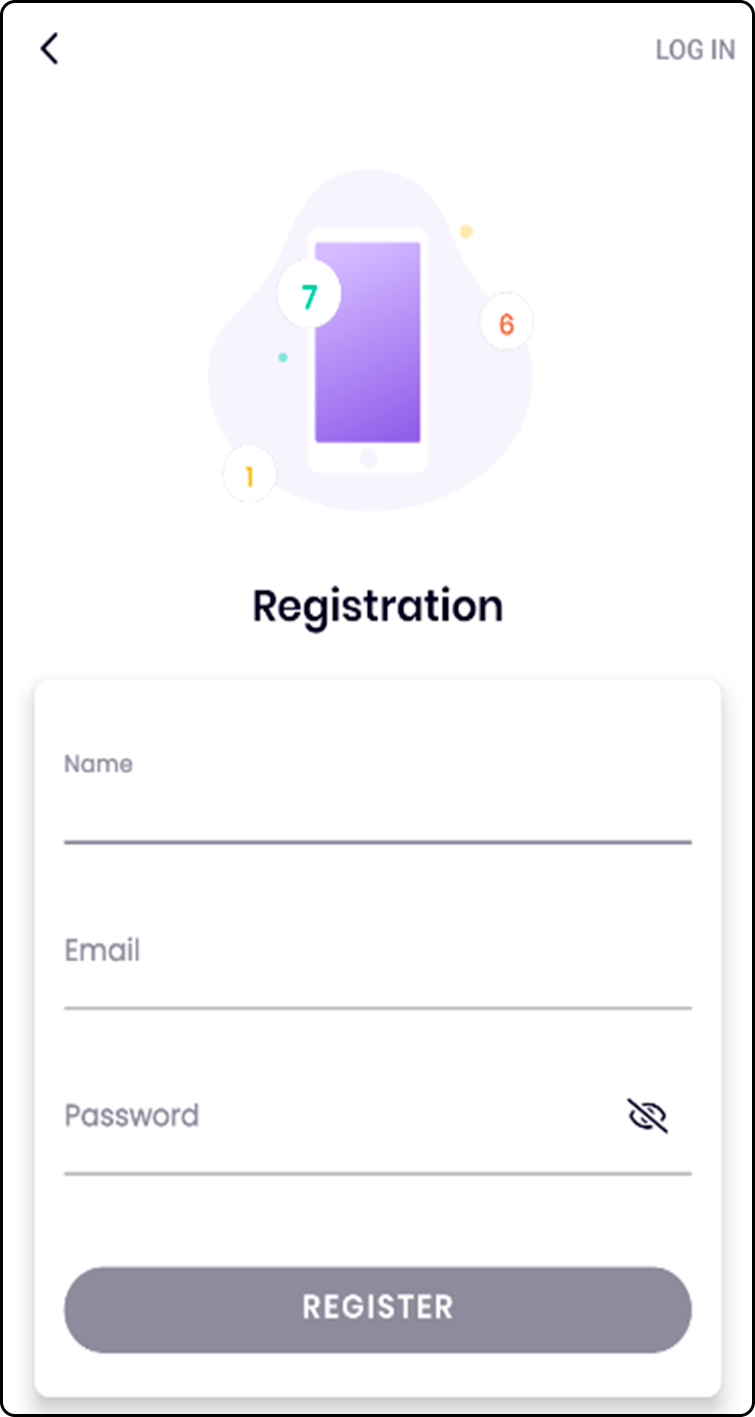
\includegraphics[scale=0.8]{auth_3.png} 
   \caption{Фрагмент регистрации пользователя}
   \label{fig:arch:auth_3}
\end{figure}

Пользователь нажимая на кнопку Register вызывает метод register, который производит базовую валидацию полей и делает запрос на регистрацию пользователя в Firebase Auth (см. листинг~\ref{lst:auth_sign_up_uc}).
\begin{lstlisting}[language=Java,label={lst:auth_sign_up_uc},caption={SignUp}]
    override suspend fun signUp(email: String, password: String, name: String) {
        return suspendCoroutine { cont ->
            auth.createUserWithEmailAndPassword(email, password)
                .addOnCompleteListener {
                    if (it.isSuccessful) {
                        auth.currentUser?.updateProfile(
                            UserProfileChangeRequest.Builder().setDisplayName(name).build()
                        )
                        cont.resume(Unit)
                    } else {
                        cont.resumeWithException(Exception(if (it.exception != null) it.exception!!.message else "Wrong login or password"))
                    }
                }
        }
    }
\end{lstlisting}

Стоит заметить, что данный метод инкапсулирует в себе еще один запрос на изменения профиля пользователя, так как изначально регистрация проходит только с полями емейла и пароля, поэтому требуется дополнительный запрос на смену профиля при завершении регистрации.

\subsubsection{Модуль исследования}~\par
Модуль исследования позволяет пользователю просмотреть самые интересные новинки и новости из мира игр за последнее время. Модуль состоит из ExploreFragment, который является основным фрагментом в данном модуле и StoryFragment, показывающий истории наподобии Instagram. Примеры пользовательского интерфейса представлены на рисунках~\ref{fig:arch:explore_1} и ~\ref{fig:arch:explore_2}.

\begin{figure}[H]
 \centering
   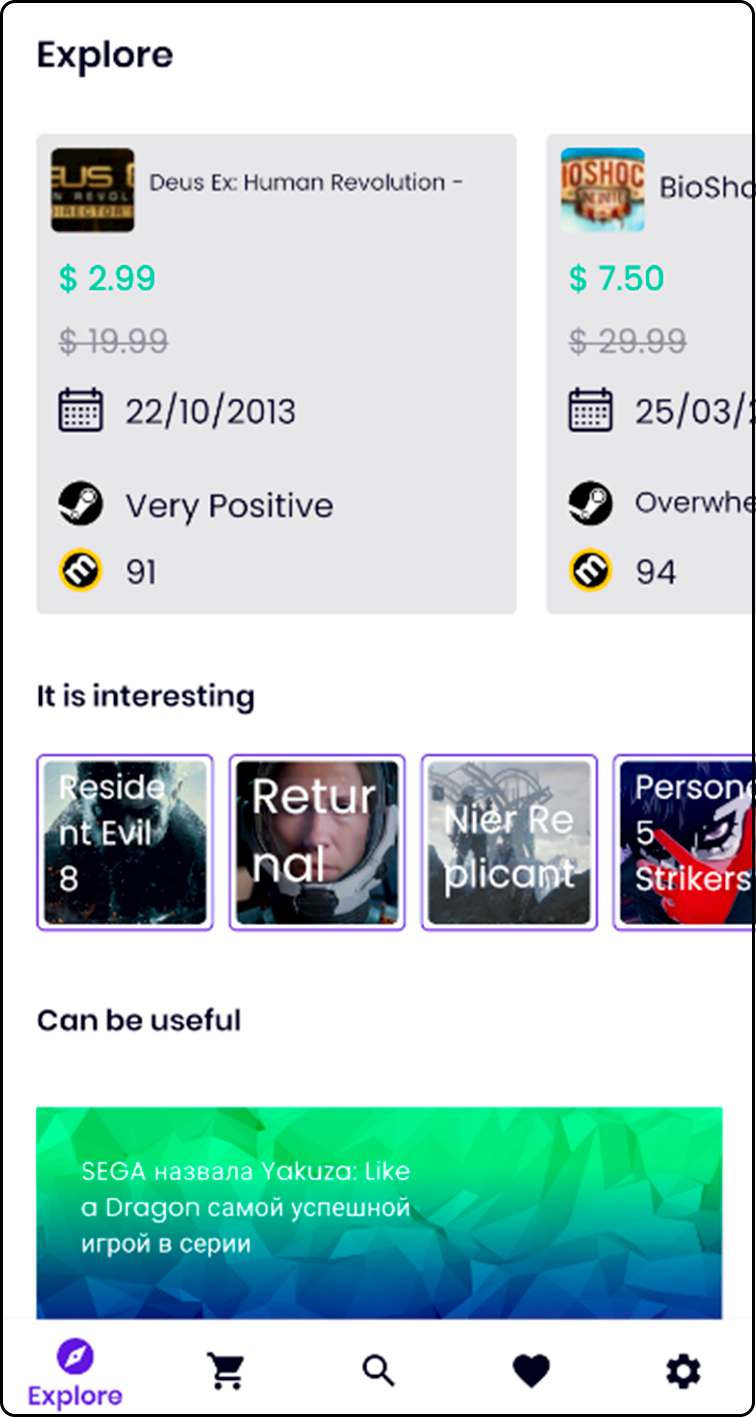
\includegraphics[scale=0.8]{explore_1.png} 
   \caption{ExploreFragment}
   \label{fig:arch:explore_1}
\end{figure}

\begin{figure}[H]
 \centering
   
\includegraphics[scale=0.8]{explore_2.png} 
   \caption{ExploreFragment}
   \label{fig:arch:explore_2}
\end{figure}

Экран исследования состоит из трёх блоков:

\begin{itemize}
  \item список игр проходящий ранжирование через фильтр рейтинга, отображаются игры с рейтингом выше 90 по Metacritic;
  \item список историй с последними новинками, позволяющий изучить как выглядит игра и перейти по ссылке для поления большей информации;
  \item колонка статей с посленими новостями из мира игр.
\end{itemize}

Список игр релизован через постраничное получение игр с сервера для оптимизации интерфейса. Когда пользователь долистывает до конца списка, то приложение делает запрос на следующую страницу игр и отображает её в исходном списке. Основным моментом в программной реализации является DealsPagingSource (см. листинг~\ref{lst:explore_paging_deals}), который выполняет подсчет страниц и обработку ошибок для каждой отдельной страницы.

\begin{lstlisting}[language=Java,label={lst:explore_paging_deals},caption={DealsPagingSource}]
class DealsPagingSource(
    private val getDeals: GetDeals,
    private val title: String? = null,
    private val ids: List<String>? = null,
    private val metacritic: Int? = null
) : PagingSource<Int, Deal>() {
    override fun getRefreshKey(state: PagingState<Int, Deal>): Int? {
        return state.anchorPosition
    }

    override suspend fun load(params: LoadParams<Int>): LoadResult<Int, Deal> {
        return try {
            val startNumber = params.key ?: 0
            val endNumber = startNumber + 1
            val response = getDeals(startNumber, title, ids, metacritic)

            LoadResult.Page(
                data = response,
                prevKey = null,
                nextKey = if (response.isEmpty()) null else endNumber
            )
        } catch (e: Exception) {
            LoadResult.Error(e)
        }
    }
}
\end{lstlisting}

Истории реализованы наподобии Instagram, при нажатии на отдельную историю открывается отдельный фрагмент StoryFragment. Программная реализация включает в себя обработку жестов нажатий для переключения историй вперед и назад, данная логика реализуется с помощью класса GestureDetectorCompat (см. листинг~\ref{lst:explore_touch}). По нажатию на экран данный класс получает координаты нажатия, после этого происходит сравнение с шириной экрана, после данного действия алгоритм решает пролистать назад истории или вперед.

\begin{lstlisting}[language=Java,label={lst:explore_touch},caption={GestureDetectorCompat}]
        val gesture =
            GestureDetectorCompat(
                requireContext(),
                object : GestureDetector.OnGestureListener {
                    override fun onDown(e: MotionEvent?): Boolean {
                        return true
                    }

                    override fun onShowPress(e: MotionEvent?) {
                    }

                    override fun onSingleTapUp(e: MotionEvent?): Boolean {
                        e?.let {
                            val x = e.x

                            if (x < (binding.vImage.width * 0.5)) {
                                binding.vProgress.previous()
                            } else {
                                binding.vProgress.next()
                            }
                        }
                        return true
                    }

                    override fun onScroll(
                        e1: MotionEvent?,
                        e2: MotionEvent?,
                        distanceX: Float,
                        distanceY: Float
                    ): Boolean {
                        return true
                    }

                    override fun onLongPress(e: MotionEvent?) {
                    }

                    override fun onFling(
                        e1: MotionEvent?,
                        e2: MotionEvent?,
                        velocityX: Float,
                        velocityY: Float
                    ): Boolean {
                        return true
                    }
                }
            )

        binding.vImage.setOnTouchListener(object : View.OnTouchListener {
            override fun onTouch(v: View?, event: MotionEvent?): Boolean {
                return gesture.onTouchEvent(event)
            }
        })
\end{lstlisting}

Блок последних новостей выполнен в виде вертикального списка с переходом на статью по нажатию на отдельный элемент списка. Получение списка новостей происходит с помощью запроса на отдельный сервер, где хранятся все последние новости игровой индустрии. Данные лежат в формате XML, соответственно преобразование данных происходит из этого формата с помощью SimpleXmlConverter из библиотеки Retrofit. Данный формат требует отдельной обработки в доменных классах приложения, рассмотрим класс RssChannel (см. листинг~\ref{lst:explore_rss}). В данном классе используются аннотации @Root, @Element, @ElementList, что соответствуют отдельным элементам целевого XML файла и позволяет XML преобразователю правильно обрабатывать файлы и переносить их в доменную область приложения. 

\begin{lstlisting}[language=Java,label={lst:explore_rss},caption={RssChannel}]
@Root(name = "channel", strict = false)
public class RssChannel
{
    @Element
    private String title;

    @Element
    private RssImage image;

    @ElementList(inline = true, required = false)
    public List<RssItem> item;

    @Override
    public String toString() {
        return "Channel [image=" + image + ", item=" + item + "]";
    }
}
\end{lstlisting}

\subsubsection{Модуль избранного}~\par
Экран избранного состоит из двух вкладок Deals и Games. Данные вкладки показывают все понравившиеся пользователю предложения по играм и сами игры. Добавление в избранное реализовано сохранением в локальную базу данных необходимых для отображения полей с индентификатором пользователя который добавил эти предложения в избранное. Примеры пользовательского интерфейса представлены на рисунках~\ref{fig:arch:favorites_1} и ~\ref{fig:arch:favorites_2}.

\begin{figure}[H]
 \centering
   
\includegraphics[scale=0.8]{favorites_1.png} 
   \caption{FavoritesFragment}
   \label{fig:arch:favorites_1}
\end{figure}

\begin{figure}[H]
 \centering
   
\includegraphics[scale=0.8]{favorites_2.png} 
   \caption{FavoritesFragment}
   \label{fig:arch:favorites_2}
\end{figure}

Помимо списков, в реализации присутствуют отдельные методы для загрузки картинок с помощью библиотеки Glide. В работе написано множество методов для их загрузки с множеством опций в классе UriBindingAdapter (см. листинг~\ref{lst:favorites_images}). Класс реализует одну из функций основных библиотек Android - DataBinding. Данная функциональность позволяет использовать методы прямо в коде интерфейса XML, что является удобным сокращением и повышает переиспользуемость методов.

\begin{lstlisting}[language=Java,label={lst:favorites_images},caption={UriBindingAdapter}]
object UriBindingAdapter {
    @JvmStatic
    @BindingAdapter(value = ["image_uri"])
    fun setUri(imageView: ImageView, url: Uri?) {
        Glide.with(imageView)
            .load(url)
            .into(imageView)
    }

    @JvmStatic
    @BindingAdapter(value = ["image_uri", "image_placeholder"])
    fun setUriWithPlaceholder(imageView: ImageView, url: Uri?, placeholder: Drawable) {
        Glide.with(imageView)
            .load(url)
            .placeholder(placeholder)
            .fallback(placeholder)
            .into(imageView)
    }

    @JvmStatic
    @BindingAdapter(value = ["image_uri", "image_placeholder", "image_radius"])
    fun setUriWithPlaceholderRadius(
        imageView: ImageView,
        url: Uri?,
        placeholder: Drawable,
        imageRadius: Int
    ) {
        Glide.with(imageView)
            .load(url)
            .transform(CenterCrop(), RoundedCorners(imageRadius.dp))
            .placeholder(placeholder)
            .fallback(placeholder)
            .into(imageView)
    }

    @JvmStatic
    @BindingAdapter(value = ["image_res", "image_placeholder", "image_radius"])
    fun setResWithPlaceholderRadius(
        imageView: ImageView,
        @DrawableRes res: Int?,
        placeholder: Drawable,
        imageRadius: Int
    ) {
        Glide.with(imageView)
            .load(res)
            .transform(CenterCrop(), RoundedCorners(imageRadius.dp))
            .placeholder(placeholder)
            .fallback(placeholder)
            .into(imageView)
    }

    @JvmStatic
    @BindingAdapter(value = ["circle_image_uri"])
    fun setCircleUri(imageView: ImageView, url: Uri?) {
        url?.let {
            Glide.with(imageView)
                .load(url)
                .circleCrop()
                .into(imageView)
        }
    }

    @JvmStatic
    @BindingAdapter(value = ["circle_image_uri", "placeholder"])
    fun setCircleUriWithPlaceholder(imageView: ImageView, url: Uri?, placeholder: Drawable) {
        url?.let {
            Glide.with(imageView)
                .load(url)
                .circleCrop()
                .placeholder(placeholder)
                .fallback(placeholder)
                .into(imageView)
        }
    }
}
\end{lstlisting}

При нажатии на сохраненную игру открывается соответствующий экран с информацией об этом предложении. Пример пользовательского интерфейса представлен на рисунке~\ref{fig:arch:favorites_3}. Данный экран включает в себя название, возможность добавить и удалить из избранного, лучшую цену за все времена, ссылку на Steam и Metacritic, а так же список магазинов в которых эту игру можно купить и по каким ценам.

\begin{figure}[H]
 \centering
   
\includegraphics[scale=0.8]{favorites_3.png} 
   \caption{Информация об игре}
   \label{fig:arch:favorites_3}
\end{figure}

Если пользователь нажмёт на сохраненное предложение, то откроется экран с деталями об этом предложении. Пример пользовательского интерфейса представлен на рисунке~\ref{fig:arch:favorites_4}. На экране предложения присутствует лучшая цена за все времена, цена игры в магазине к которому предложение соответствует, а так же индикация того, является ли это предложение лучшим среди магазинов. Если предложение является лучшим, то соответствующие сообщение показывается пользователю, если нет, то показывается список магазинов в котором эту игру можно купить по более дешевой цене.

\begin{figure}[H]
 \centering
   
\includegraphics[scale=0.8]{favorites_4.png} 
   \caption{Информация о предложении}
   \label{fig:arch:favorites_4}
\end{figure}


\subsubsection{Модуль поиска}~\par
Пользовательский интерфейс и программная реализация схожа с модулем избранного, за исключением наличия фильтров и возможности поиска. Приложение делает запросы на списки игр и предлжений вместе с фильтрами и поисковой строкой задаваемой пользователем. Стоит отметить, что поисковая строка реализована с соблюдением Google Material Design и содержит историю поисковых запросов пользователя, а так же имеет возможность голосового ввода. Пример пользовательского интерфейса истории поисковых запросов представлен на рисунке~\ref{fig:arch:search_1}.

\begin{figure}[H]
 \centering
   
\includegraphics[scale=0.8]{search_1.png} 
   \caption{История поисковых запросов}
   \label{fig:arch:search_1}
\end{figure}

\subsubsection{Модуль магазинов}~\par
Модуль магазинов реализует получения списка всех доступных магазинов и возможность включать и отключать их при работе с приложением. Если пользователь выключит с помощью нажатия на кнопку какой-либо магазин, то он больше не будет участвовать в ответах выдываемых пользователю. Магазины могут работать в режиме без подключения к сети, для этого при получении магазинов производится их кеширование в локальную базу данных. При нажатии на один из магазинов открывается страница с предложениями только этого магазина. Примеры пользовательского интерфейса представлены на рисунках~\ref{fig:arch:stores_1} и ~\ref{fig:arch:stores_2}.

\begin{figure}[H]
 \centering
   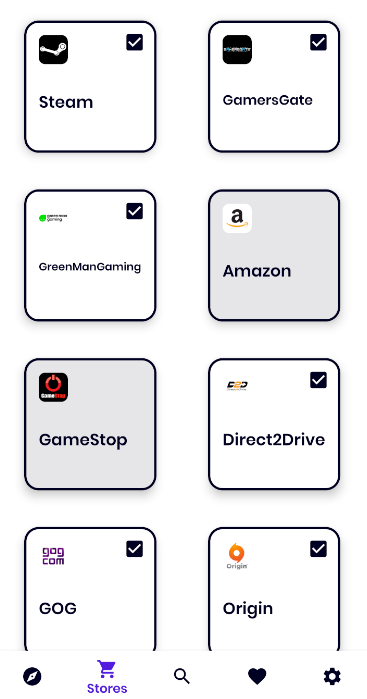
\includegraphics[scale=0.8]{stores_1.png} 
   \caption{Экран со всеми магазинами}
   \label{fig:arch:stores_1}
\end{figure}

\begin{figure}[H]
 \centering
   
\includegraphics[scale=0.8]{stores_2.png} 
   \caption{Предложения одного магазина}
   \label{fig:arch:stores_2}
\end{figure}

\subsubsection{Модуль аккаунта}~\par
Модуль относящийся к настройкам самого пользователя и социальным функциям. Данный модуль аккаунта состоит из 6 экранов.

\begin{itemize}
    \item основной экран пользователя;
    \item экран нотификаций;
    \item экран с возможностью поделиться приложением;
    \item экран с возможностью купить подписку на приложение;
    \item экран настроек;
    \item экран информации.
\end{itemize}

Основной экран пользователя выполняет роль навигации между остальными экранами и позволяет сменить аватар пользователя. Пример пользовательского интерфейса представлен на рисунке~\ref{fig:arch:account_1}.

\begin{figure}[H]
 \centering
   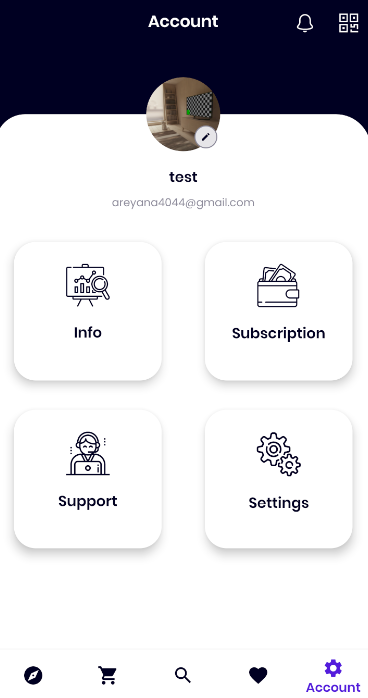
\includegraphics[scale=0.8]{account_1.png} 
   \caption{Основной экран пользователя}
   \label{fig:arch:account_1}
\end{figure}


Для данного экрана был написан набор методов по работе с камерой и галереей приложения. Пользователю доступны возможности удаления аватара, добавления его с помощью камеры или галереи приложения. Учтено отсутствия разрешний на камеру у приложения и выполнена обработка этой ситуации с помощью запрашивания этого разрешения у пользователя в виде диалога. Если пользователь отклонил 2 раза запрос разрешения на доступ к камере, то в следующие разы он будет получать сообщение о просьбе перехода на экран настроек приложения в системе Android и ручного добавления разрешения, данное действие происходит с помощью метода openSettingsPermissionAppActivity (см. листинг~\ref{lst:camera_methods}).
\begin{lstlisting}[language=Java,label={lst:camera_methods},caption={Методы для взаимодействия с камерой}]
private fun dispatchTakePictureFromCameraIntent() {
        avatarUri =
            getOutputMediaFile("avatar_${OffsetDateTime.now().toInstant().toEpochMilli()}.jpg")
        openTakePictureFromCamera.launch(avatarUri)
    }

    private val openTakePictureFromCamera =
        registerForActivityResult(ActivityResultContracts.TakePicture()) { result ->
            if (result) {
                viewModel.addAvatarEvent(avatarUri!!)
            }
        }

    private val openTakePictureFromGallery =
        registerForActivityResult(ActivityResultContracts.GetContent()) { result ->
            avatarUri = result
            viewModel.addAvatarEvent(avatarUri!!)
        }

    private val checkCameraPermission =
        registerForActivityResult(ActivityResultContracts.RequestPermission()) { result ->
            if (result) {
                dispatchTakePictureFromCameraIntent()
            } else {
                if (!shouldShowRequestPermissionRationale(Manifest.permission.CAMERA)) {
                    openGoToSettingPermissionDialog(openSettingsPermissionAppActivity)
                }
            }
        }

    private val openSettingsPermissionAppActivity: ActivityResultLauncher<Intent> =
        registerForActivityResult(ActivityResultContracts.StartActivityForResult()) {
            checkCameraPermission.launch(Manifest.permission.CAMERA)
        }
\end{lstlisting}

Одна из социальных функций приложения представлена в виде экрана с возможностью поделиться ссылкой на приложение в сообщении, либо QR кодом. Пример пользовательского интерфейса представлен на рисунке~\ref{fig:arch:account_5}.

\begin{figure}[H]
 \centering
   
\includegraphics[scale=0.8]{account_5.png} 
   \caption{Экран с возможностью поделиться приложением}
   \label{fig:arch:account_5}
\end{figure}

С помощью нативного класса ShareCompat, был реализован метод по отправке ссылки на приложение. Ссылка может быть отправлена в любое приложение которое поддерживает тип test/plain (см. листинг~\ref{lst:share_method}).
\begin{lstlisting}[language=Java,label={lst:share_method},caption={Методы для отправки ссылки на приложение}]
            val shareItem = menu.findItem(R.id.menuShare)
            shareItem.setOnMenuItemClickListener {
                ShareCompat.IntentBuilder(requireContext())
                    .setType("text/plain")
                    .setChooserTitle("Choose one")
                    .setText("http://play.google.com/store/apps/details?id=" + requireActivity().packageName)
                    .startChooser()
                return@setOnMenuItemClickListener true
            }
\end{lstlisting}

В работе одним из самых важных экранов является экран настроек. Пример пользовательского интерфейса представлен на рисунке~\ref{fig:arch:account_2}. На экране присутствует список переходов и переключателей, данный список реализован с помощью библиотеки Groupie. Библиотека нужна для более удобного добавления новых опций в список без изменения большого количества кода.

\begin{itemize}
    \item переключатель Notification, включает и отключает доступ к нотификациям у приложения;
    \item переключатель Show inactive stores, изменяет видимость недоступных в данный момент магазинов в приложении;
    \item переход Language, осуществляет навигацию на экран смены языка приложения;
    \item переключатель Night mode, переключает с темной на светлую тему приложения и обратно;
    \item переходы Privacy policy и Terms of service, осуществляют навигацию на страницы с юридической информацией;
    \item переход Sign Out выполняет выход пользователя из приложения на модуль авторизации.
\end{itemize}

\begin{figure}[H]
 \centering
   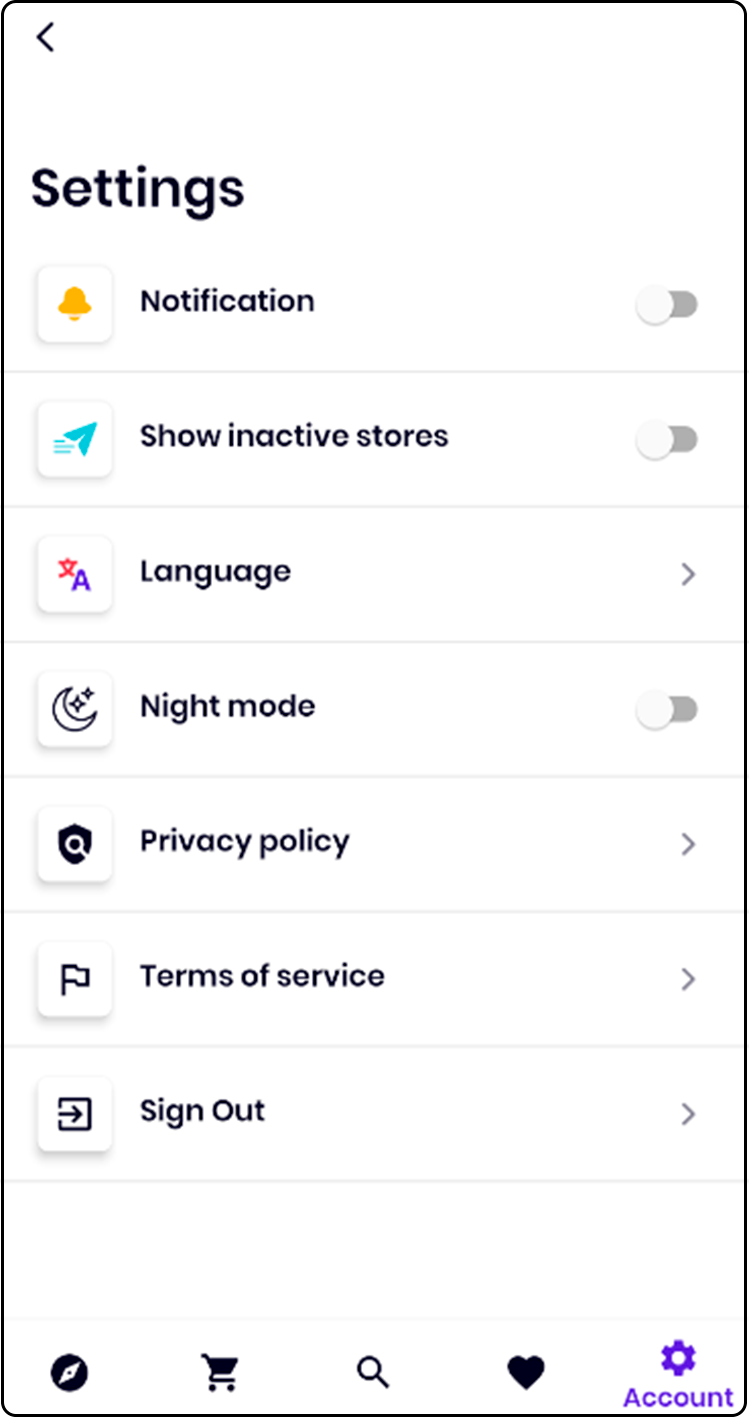
\includegraphics[scale=0.8]{account_2.png} 
   \caption{Экран настроек}
   \label{fig:arch:account_2}
\end{figure}

Каждая из настроек синхронизируется с Firestore для каждого пользователя, что позволяет сохранять состояние настроек на разных устройствах под одним аккаунтом. Например, для настройки Notification используется ключ notification под которым для каждого отдельного пользователя записывается состояние этой настройки с помощью методов putNotification и getNotification  (см. листинг~\ref{lst:prefs_notification}).

\begin{lstlisting}[language=Java,label={lst:prefs_notification},caption={Методы для Notification}]
    override suspend fun putNotification(boolean: Boolean) {
        return suspendCoroutine { cont ->
            val uid = auth.currentUser?.uid!!
            val users = db.collection(usersKey).document(uid)
            val map: Map<String, Boolean> = mapOf(notificationsKey to boolean)
            users.set(map, SetOptions.merge()).addOnCompleteListener {
                cont.resume(Unit)
            }.addOnCanceledListener {
                cont.resumeWithException(Exception("No Connection"))
            }
        }
    }

    override suspend fun getNotification(): Boolean {
        return suspendCoroutine { cont ->
            val uid = auth.currentUser?.uid!!
            val users = db.collection(usersKey).document(uid)
            users.get().addOnCompleteListener {
                if (it.isSuccessful && it.result != null) {
                    val result = it.result!!
                    if (result.contains(notificationsKey)) {
                        cont.resume(result[notificationsKey] as Boolean)
                    } else {
                        cont.resume(false)
                    }
                } else {
                    cont.resumeWithException(Exception("No Connection"))
                }
            }.addOnCanceledListener {
                cont.resumeWithException(Exception("No Connection"))
            }
        }
    }
\end{lstlisting}

На экране информации пользователь может прочитать о приложении и перейти по ссылкам чтобы получить связанную с разработчиком информацию, например на сервер Discord или в PlayStore. Переход по ссылкам осуществляется с помощью browserIntent, намерения с помощью которого система открывает ссылку в доступном браузере (см. листинг~\ref{lst:prefs_intent}).

\begin{lstlisting}[language=Java,label={lst:prefs_intent},caption={browserIntent}]
        val browserIntent = Intent(Intent.ACTION_VIEW, Uri.parse("http://play.google.com/store/apps/dev?id=areyanainc"))
        startActivity(browserIntent)
\end{lstlisting}

\subsection{Безопасность}
Для обеспечения безопасности чувствительных данных была использована Android библиотека Security для шифрования пользовательских настроек приложения. Логика по взаимодействию с этой библиотекой реализована в классе PreferenceDataSource (см. листинг~\ref{lst:prefs_security}).

\begin{lstlisting}[language=Java,label={lst:prefs_security},caption={PreferenceDataSource}]
class PreferenceDataSource(val context: Context) {

    private val masterKeyAlias = MasterKey
        .Builder(context)
        .setKeyScheme(MasterKey.KeyScheme.AES256_GCM)
        .build()

    private val cryptoPreferences = EncryptedSharedPreferences.create(
        context,
        "secret_shared_prefs",
        masterKeyAlias,
        EncryptedSharedPreferences.PrefKeyEncryptionScheme.AES256_SIV,
        EncryptedSharedPreferences.PrefValueEncryptionScheme.AES256_GCM
    )

    private val notifications: String = context.getString(R.string.pref_notifications)
    private val notificationsDefault: Boolean =
        context.getString(R.string.pref_notifications_default).toBoolean()
    var notificationsEnabled: Boolean
        get() = cryptoPreferences.getBoolean(notifications, notificationsDefault)
        set(value) {
            val editor = cryptoPreferences.edit()
            editor.putBoolean(notifications, value)
            editor.apply()
        }

    private val needToShowOnboarding: String =
        context.getString(R.string.pref_need_to_show_onboarding)
    private val needToShowOnboardingDefault: Boolean =
        context.getString(R.string.pref_need_to_show_onboarding_default).toBoolean()
    var onboardingEnabled: Boolean
        get() = cryptoPreferences.getBoolean(needToShowOnboarding, needToShowOnboardingDefault)
        set(value) {
            val editor = cryptoPreferences.edit()
            editor.putBoolean(needToShowOnboarding, value)
            editor.apply()
        }
}
\end{lstlisting}

На серверной стороне для Firebase Storage и Firestore были написаны правила, которые не позволяют пользователям получать доступ ко всем данным, а только для их части, что соответствует их уникальному идентификатору (см. листинг~\ref{lst:firebase_security}).

\begin{lstlisting}[language=Javascript,label={lst:firebase_security},caption={Правила Firestore}]
rules_version = '2';
service cloud.firestore {
  match /databases/{database}/documents {
     match /users/{userId}/{document=**} {
      allow read, update, delete, create: if request.auth.uid == userId;
    }
  }
}
\end{lstlisting}


\subsection{Варианты использования}
Далее будут рассмотрены основные варианты использования разработанного мобильного приложения.

\subsubsection{ВИ Создание учётной записи}~\par
\label{use:reg}
Описание ВИ: Пользователь имеет возможность при желании создать личную учётную запись.
 
Предусловия основного потока действий нет.
 
Основной поток действий:
\begin{itemize}
   \item пользователь нажимает кнопку "Register";
   \item пользователь вводит электронную почту, имя пользователя, пароль.
\end{itemize}
 
Ограничения: различные ограничения, установленные провайдером аутентификации Firebase, а так же клиентским приложением.
 
\subsubsection{ВИ Использование своей учётной записи}~\par
Описание ВИ: Пользователь имеет возможность использовать личную учётную запись.
 
Предусловия основного потока действий: у пользователя имеется учётная запись см.~\ref{use:reg}.
 
Основной поток действий:
\begin{itemize}
   \item пользователь нажимает кнопку "SIGN IN";
   \item пользователь вводит электронную почту и пароль.
\end{itemize}
 
Ограничения: различные ограничения, установленные провайдером аутентификации Firebase, а так же клиентским приложением.

\subsubsection{ВИ Восстановление пароля}~\par
\label{use:resetpassword}
Описание ВИ: Пользователь имеет возможность восстановить пароль для своей учетной записи.
 
Предусловия основного потока действий: пользователь должен быть зарегистрирован.
 
Основной поток действий:
\begin{itemize}
   \item пользователь нажимает кнопку "Forgot password?";
   \item пользователь вводит емейл своей учетной записи;
   \item клиент получает письмо на емейл с восстановлением пароля.
\end{itemize}
 
Ограничения: емейл должен быть валидным и не пустым.
 
\subsubsection{ВИ Просмотр истории}~\par
Описание ВИ: Пользователь имеет возможность просмотреть историю о вышедшей новинке.
 
Предусловия основного потока действий: у пользователя имеется учётная запись см.~\ref{use:reg}.
 
Основной поток действий:
\begin{itemize}
   \item пользователь нажимает на историю;
   \item пользователь получает на экран изображения игры в виде историй из Instagram;
   \item пользователь может совершать навигацию между изображениями с помощью жестов.
\end{itemize}
 
Ограничений нет.

\subsubsection{ВИ Просмотр статьи}~\par
\label{use:join}
Описание ВИ: Пользователь имеет возможность просмотреть свежую статью об игровой индустрии.
 
Предусловия основного потока действий: у пользователя имеется учётная запись см.~\ref{use:reg}.
 
Основной поток действий:
\begin{itemize}
   \item пользователь нажимает на статью;
   \item приложение открывает браузер со статьей.
\end{itemize}
 
Ограничения: пользователь должен иметь подключение к интернету.
 
\subsubsection{ВИ Просмотр предложения}~\par
Описание ВИ: Пользователь имеет возможность просмотреть дополнительную информацию о предложении.
 
Предусловия основного потока действий: у пользователя имеется учётная запись см.~\ref{use:reg}.

Основной поток действий:
\begin{itemize}
   \item пользователь нажимает на предложение;
   \item приложение совершает навигацию на страницу о дополнительной информации о предложении;
   \item приложение делает запрос о дополнительной информации о предложении;
   \item пользователь может просматривать дополнительную информацию о предложении, в виде скидок, более выгодных предложений, рейтинга.
\end{itemize}
 
Ограничения: пользователь должен иметь подключение к интернету.
 
\subsubsection{ВИ Просмотр игры}~\par
Описание ВИ: Пользователь имеет возможность просмотреть дополнительную информацию об игре.
 
Предусловия основного потока действий: у пользователя имеется учётная запись см.~\ref{use:reg}.

Основной поток действий:
\begin{itemize}
   \item пользователь нажимает на игру;
   \item приложение совершает навигацию на страницу о дополнительной информации о игре;
   \item приложение делает запрос о дополнительной информации об игре;
   \item пользователь может просматривать дополнительную информацию об игре, в виде скидок, предложений, рейтинга.
\end{itemize}
 
Ограничения: пользователь должен иметь подключение к интернету.
 
\subsubsection{ВИ Просмотр списка магазинов}~\par
\label{use:showstores}
Описание ВИ: Пользователь имеет возможность просмотреть все магазины доступные в приложении.
 
Предусловия основного потока действий: у пользователя имеется учётная запись см.~\ref{use:reg}.
 
Основной поток действий:
\begin{itemize}
   \item пользователь открывает список магазинов;
   \item приложение делает запрос на список магазинов;
   \item пользователь может просматривать список магазинов.
\end{itemize}
 
Ограничения: пользователь должен иметь подключение к интернету.

\subsubsection{ВИ Просмотр отдельного магазина}~\par
\label{use:singlestore}
Описание ВИ: Пользователь имеет возможность просмотреть предложения конкретного магазина.
 
Предусловия основного потока действий: у пользователя имеется учётная запись см.~\ref{use:reg}, Пользователь просматривает список магазинов см.~\ref{use:showstores}.
 
Основной поток действий:
\begin{itemize}
   \item пользователь нажимает на отдельный магазин;
   \item приложение делает запрос на список предложений от конкретного магазина;
   \item пользователь может просматривать и выбирать предложения.
\end{itemize}
 
Ограничения: пользователь должен иметь подключение к интернету.

\subsubsection{ВИ Выключение магазина из фильтрации}~\par
Описание ВИ: Пользователь имеет возможность выключить магазин из фильтрации в приложении.
 
Предусловия основного потока действий: у пользователя имеется учётная запись см.~\ref{use:reg}, Пользователь просматривает список магазинов см.~\ref{use:showstores}.
 
Основной поток действий:
\begin{itemize}
   \item пользователь нажимает на "галочку", тем самым выключая магазин из фильтрации;
   \item приложение запоминает выбор пользователя.
\end{itemize}

Альтернативный поток действий:
\begin{itemize}
   \item пользователь нажимает на "галочку", тем самым включая магазин в фильтрацию;
   \item приложение запоминает выбор пользователя.
\end{itemize}
 
Ограничений нет.

\subsubsection{ВИ Поиск игр}~\par
\label{use:searchgames}
Описание ВИ: Пользователь имеет возможность совершать поиск по играм с помощью поисковой строки и фильтров.
 
Предусловия основного потока действий: у пользователя имеется учётная запись см.~\ref{use:reg}.
 
Основной поток действий:
\begin{itemize}
   \item пользователь открывает поиск;
   \item приложение делает запрос на список игр;
   \item пользователь вводит в поисковую строку значения и выбирает фильтр;
   \item пользователь может просматривать список отфильтрованных игр.
\end{itemize}
 
Ограничения: пользователь должен иметь подключение к интернету.

\subsubsection{ВИ Поиск предложений}~\par
\label{use:searchdeals}
Описание ВИ: Пользователь имеет возможность совершать поиск по предложениям с помощью поисковой строки и фильтров.
 
Предусловия основного потока действий: у пользователя имеется учётная запись см.~\ref{use:reg}.
 
Основной поток действий:
\begin{itemize}
   \item пользователь открывает поиск;
   \item приложение делает запрос на список предложений;
   \item пользователь вводит в поисковую строку значения и выбирает фильтр;
   \item пользователь может просматривать список отфильтрованных предложений.
\end{itemize}
 
Ограничения: пользователь должен иметь подключение к интернету.

\subsubsection{ВИ Добавление предложения в избранное}~\par
\label{use:favoritedeals}
Описание ВИ: Пользователь имеет возможность добавить в избранное предложение.
 
Предусловия основного потока действий: у пользователя имеется учётная запись см.~\ref{use:reg}, Пользователь совершил поиск по предложениям см.~\ref{use:searchdeals}.
 
Основной поток действий:
\begin{itemize}
   \item пользователь нажимает на предложение из списка;
   \item пользователь нажимает на "сердце" и добавляет предложение в избранное.
   \item приложение запоминает выбор пользователя.
\end{itemize}

Альтернативный поток действий:
\begin{itemize}
   \item пользователь нажимает на предложение из списка;
   \item пользователь нажимает на "сердце" и удаляет предложение из избранного.
   \item приложение запоминает выбор пользователя.
\end{itemize}

Ограничения: пользователь должен иметь подключение к интернету.

\subsubsection{ВИ Добавление игры в избранное}~\par
\label{use:favoritegames}
Описание ВИ: Пользователь имеет возможность добавить в избранное игру.
 
Предусловия основного потока действий: у пользователя имеется учётная запись см.~\ref{use:reg}, Пользователь совершил поиск по играм см.~\ref{use:searchgames}.
 
Основной поток действий:
\begin{itemize}
   \item пользователь нажимает на игру из списка;
   \item пользователь нажимает на "сердце" и добавляет игру в избранное.
   \item приложение запоминает выбор пользователя.
\end{itemize}

Альтернативный поток действий:
\begin{itemize}
   \item пользователь нажимает на игру из списка;
   \item пользователь нажимает на "сердце" и удаляет игру из избранного.
   \item приложение запоминает выбор пользователя.
\end{itemize}

Ограничения: пользователь должен иметь подключение к интернету.

\subsection{Тестирование приложения}
Для оптимизации мобильного приложения использовалось ПО из проекта Leak Canary. В рамках данного проекта разработан набор различных программ, которые помогают автоматизировать процесс тестирования мобильных приложений. Для данного проекта использовались JUnit и Espresso - универсальные библиотеки для тестирования мобильных приложений.
 
Также было проведено ручное тестирование приложения, так как при помощи тестов Android некоторые моменты протестировать затруднительно. В рамках ручного тестирования было проведено дымовое тестирование возможностей приложения и механизмов синхронизации.


%Примеры пользовательского интерфейса представлены на рисунках~\ref{fig:arch:main_page} и~\ref{fig:arch:room_page}.
%Для воспроизведения видео используется тег <video>, который был введён в стандарте HTML5.
%
%Данный стандарт определяет для тега <video> ряд атрибутов и событий, для контроля воспроизведения.
%Проблема заключается в том, что стандартные элементы управления тега <video> не обладают всеми необходимыми возможностями для реализации данного проекта.
%Также при помощи JS кода нет никакой возможности изменить события при взаимодействии со стандартные элементы управления. 
%Можно только добавить собственную логику, которая будет работать после выполнения стандартной.
%Данное ограничение делает невозможным реализацию хорошей синхронизации, так как у пользователя инициировавшего событие оно произойдёт сразу, а у остальных после %получения данных с сервера.
%
%Для решения проблемы синхронизации был реализован собственный пользовательский интерфейс (см. рис.~\ref{fig:arch:room_page}), который позволяет полностью манипулировать %порядком выполняемых действий. Реализация данного пользовательского интерфейса представлена в листинге~\ref{lst:player}.
%\begin{lstlisting}[language=JavaScript,label={lst:player},caption={Компонент Player}]
%    import React, { Component } from 'react';
%    import { MdPlayArrow, MdPause, MdFullscreen, MdQueue } from 'react-icons/md';
%    import './player.scss';
%    import TimeIndicator from './TimeIndicator';
%    import RangeBar from './Slider';
%    import Hotkeys from 'react-hot-keys';
%    import VolumeSlider from './VolumeSlider';
%    import { PlayerBackend } from '../PlayerBackend/default';
%    import PlayList from './PlayList';
%    import Notifications from './Notifications';
%    import Chat from './Chat';
%     
%    const pauseIcon = <MdPause />;
%    const playIcon = <MdPlayArrow />;
%     
%    class Player extends Component {
%       constructor(props) {
%           super(props);
%           this.processor = new PlayerBackend();
%           this.playerElemetn = React.createRef();
%           this.state = {
%               isFullscreen: false,
%               playbackIcon: playIcon,
%               playbackState: false,
%               playlist: false,
%               showVideoChooser: false,
%               showChat: false,
%           }
%       }
%     
%       componentDidMount() {
%           this.vid_title = document.getElementById('video-title');
%           this._connectToPlayerBackend();
%           document.onfullscreenchange = () => this.setState({ isFullscreen: !this.state.isFullscreen });
%           if (this.props.externalSetUp) {
%               for (const func of this.props.externalSetUp) {
%                   func(this.processor);
%               }
%           }
%       }
%     
%       _connectToPlayerBackend = () => {
%           this.processor.video = document.getElementById('video-player');
%           this.setState({ time: this.processor.time, volume: this.processor.volume })
%     
%           this.processor.video.addEventListener('timeupdate', () => this.setState({ time: this.processor.time }));
%           this.processor.video.addEventListener('volumechange', () => this.setState({ volume: this.processor.volume }));
%     
%           for (const event in this.props.events) {
%               this.processor.addPreAction(this.props.events[event], event);
%           }
%       }
%     
%       playback = () => {
%           this.processor.dispatch('changePlayback', this.processor.paused);
%           this.processor.dispatch('setTime', this.processor.time);
%           let newIcon = this.processor.paused ? pauseIcon : playIcon;
%           this.setState({ playbackIcon: newIcon, playbackState: this.processor.paused });
%       }
%     
%       fullscreen = () => {
%           if (this.state.isFullscreen) {
%               this.leaveFullscreen();
%           } else {
%               this.enterFullscreen();
%           }
%       }
%     
%       enterFullscreen = () => {
%           const elem = this.playerElemetn.current;
%           if (elem.requestFullscreen) {
%               elem.requestFullscreen();
%           } else if (elem.mozRequestFullScreen) {
%               elem.mozRequestFullScreen();
%           } else if (elem.webkitRequestFullscreen) {
%               elem.webkitRequestFullscreen();
%           } else if (elem.msRequestFullscreen) {
%               elem.msRequestFullscreen();
%           }
%       }
%     
%       leaveFullscreen = () => {
%           if (document.exitFullscreen) {
%               document.exitFullscreen();
%           } else if (document.mozCancelFullScreen) {
%               document.mozCancelFullScreen();
%           } else if (document.webkitExitFullscreen) {
%               document.webkitExitFullscreen();
%           } else if (document.msExitFullscreen) {
%               document.msExitFullscreen();
%           }
%       }
%     
%       setTime = (timeValue) => {
%           if (!timeValue.isNaN) {
%               this.processor.dispatch('setTime', timeValue * this.processor.duration);
%           }
%       }
%     
%       setVolume = (volumeValue) => {
%           this.processor.dispatch('setVolume', volumeValue);
%       }
%     
%       changeMute = () => {
%           this.processor.dispatch('changeMute');
%       }
%     
%     
%       togglePlaylist = () => {
%           this.setState({ playlist: !this.state.playlist });
%       }
%     
%       toogleChat = (e) => {
%           this.setState({ showChat: !this.state.showChat });
%       }
%     
%       render() {
%           return (
%               <div className='player-wrapper' id='player' ref={this.playerElemetn}>
%                   <Hotkeys keyName='space' onKeyUp={this.playback} />
%                   <Hotkeys keyName='c' onKeyUp={this.toogleChat} />
%                   <div className='player-layer'>
%                       <video id='video-player' />
%                   </div>
%     
%                   <div className='player-layer mouse-show'>
%                       <div id='player-controls' className='player-controls'>
%                           <div className='player-controls-row'>
%                               <RangeBar value={this.processor.timeProgress} handle_change={this.setTime} style={{ 'margin-top': '5px', 'margin-bottom': '5px' }} />
%                           </div>
%                           <div className='player-controls-row'>
%                               <div onClick={this.playback} className="player-button player-button-play">
%                                   {this.state.playbackIcon}
%                               </div>
%                               <VolumeSlider volume={this.state.volume} volumeHandler={this.setVolume} toggleMute={this.changeMute} />
%                               <TimeIndicator time={this.processor.time} duration={this.processor.duration} />
%                               <div className='player-button' onClick={this.togglePlaylist}>
%                                   <MdQueue />
%                               </div>
%                               <div id='fullscreen-btn' onClick={this.fullscreen} className="player-button player-button-fullscreen">
%                                   <MdFullscreen />
%                               </div>
%                           </div>
%                       </div>
%                   </div>
%                   <Notifications />
%                   <PlayList processor={this.processor} visibility={this.state.playlist} playlistLogic={this.props.playlistLogic} libraryLogic={this.props.libraryLogic} %toogleVideoChooser={this.toogleVideoChooser} />
%                   {this.state.showChat &&
%                       <div className='player-layer'>
%                           <Chat hide={this.toogleChat}/>
%                       </div>
%                   }
%               </div>
%           );
%       }
%    }
%     
%    export default Player;
%\end{lstlisting}
%
%Данный компонент содержит внутри себя несколько дочерних компонентов: PlayList, VolumeSlider, TimeIndicator, RangeBar. 
%Это сделано с целью оптимизации работы с деревом DOM, так как данные элементы должны регулярно обновляться.
%
%Элементы управления компонента Player обрабатывают определённые события (пауза, перемотка и т.д.). 
%Для непосредственного управления тегом <video> реализован дополнительный класс PlayerBackend (см. листинг~\ref{lst:playerback}), который содержит логику для управления %процессом воспроизведения. При помощи данного класса можно управлять видео напрямую, вызывая событие сразу, или использовать метод dispatch, который занимается %обработкой последовательности событий.
%Данный метод необходим для того, чтобы можно было модифировать стандартную логику тега <video>.
%При реализации данного метода ыл рассмотрен механизм работы библиотеки Redux, для того чтобы данный метод соответствовал Flux архитектуре.
%Для метода dispatch доступно следующие действия (actions): 
%\begin{itemize}
%    \item changePlayback (ставит видео на паузу или возобновляет воспроизведение);
%    \item setTime (перематывает видео);
%    \item setVolume (изменяет громкость видео);
%    \item changeMute (заглушает видео);
%    \item setSrc (устанавливает источник видео).
%\end{itemize}
%
%Метод dispatch позволяет выполнить дополнительное действие перед стандартным. Для этого необходимо после создания объекта данного класса вызвать метод addPreAction, %который принимает название действия и функцию, которую необходимо выполнить перед данным действием. Благодаря этому разработанный плеер можно использовать и без %синхронизации, так как синхронизирующая логика добавляется при помощи метода addPreAction.
%
%\begin{lstlisting}[language=JavaScript,label={lst:playerback},caption={Класс PlayerBackend}]
%class PlayerBackend {
% constructor(video) {
%     this._video = video;
%     this._preActions = {};
%     this._actions = {
%         'changePlayback': this.changePlayback,
%         'setTime': this.setTime,
%         'setVolume': this.setVolume,
%         'changeMute': this.changeMute,
%         'setSrc': this.setSource
%     }
% }
% 
% set video(value) {
%     this._video = value;
%     this._video.addEventListener('error', (e) => { console.error('error', e) });
%     this._video.addEventListener('waiting', (e) => { console.error('waiting', e) });
%     this._video.addEventListener('stalled', (e) => { console.error('stalled', e) });
% }
% 
% get video() {
%     return this._video;
% }
% 
% addPreAction = (value, action) => {
%     if (this._preActions[action] === undefined) {
%         this._preActions[action] = []
%     }
%     this._preActions[action].push(value);
% }
% 
% resetPreActions() {
%     this._preActions = {}
% }
% 
% resetPostActions() {
%     this._preActions = {}
% }
% 
% // Playback
% _play = () => {
%     this._video.play().catch((e) => console.error('playback', e));
% }
% 
% _pause = () => {
%     this._video.pause();
% }
% 
% get paused() {
%     return this._video.paused;
% }
% 
% changePlayback = (paused) => {
%     if (paused !== undefined) {
%         paused ? this._play() : this._pause();
%     } else {
%         this.paused ?  this._play() : this._pause();
%     }
% }
% 
% // Volume
% set volume(value) {
%     this._video.volume = value;
% }
% 
% setVolume = (value) => this._video.volume = value;
% 
% get volume() {
%     return this._video.volume;
% }
% 
% get muted() {
%     return this._video.muted;
% }
% 
% changeMute = () => {
%     this._video.muted = !this._video.muted;
% }
% 
% // Time
% setTime = (value) => this._video.currentTime = value;
%  set time(value) {
%     this._video.currentTime = value;
% }
% 
% setTime = (value) => this._video.currentTime = value;
% 
% get time() {
%     return this._video ? this._video.currentTime || 0 : 0;
% }
% 
% get timeProgress() {
%     return this._video ? this._video.currentTime / this._video.duration || 0 : 0;
% }
% 
% get duration() {
%     return this._video ? this._video.duration || 0 : 0;
% }
% 
% //  Src
% set source(value) {
%     this._video.src = value;
% }
% 
% setSource = (value) => this._video.src = value;
% 
% dispatch = (action, value) => {
%     let _preActions = this._preActions[action] || [];
%     const _actionWrapper = promiseWrapper(this._actions[action], value);
% 
%     let promise = new Promise(resolve => resolve());
%     for (const _preAction of _preActions) {
%         promise = promise.then(promiseWrapper(_preAction, value));
%     }
% 
%     promise.then(promiseWrapper(this._actions[action], value));
% }
%}
%\end{lstlisting}
%
%\subsection{Реализация синхронизирующей логики}
%Так как класс PlayerBackend позволяет выполнять основные операции для управления видео без синхронизации, для выполнения синхронизации необходимо использовать %дополнительный класс, который предоставит данную возможность. Реализация основных методов для синхронизации и работы с Firebase представлена в листинге~\ref{lst:firebase}%. 
%
%\begin{lstlisting}[language=JavaScript,label={lst:firebase},caption={Методы для взаимодействия с Firebase}]
%changePlayback = (roomId, paused) => {
% let room_ref = this.db.collection('rooms').doc(roomId);
% room_ref.update({ paused })
% return room_ref.get().then(() => 'skip');
%}
% 
%listenPlayback = (roomId, dispatcher) => {
% return this.db.collection('rooms').doc(roomId).onSnapshot(snap => {
%   if (snap.data()) {
%     dispatcher.firebaseData.paused = snap.data().paused;
%     dispatcher.changePlayback(!snap.data().paused);
% 
%   }
% });
%}
% 
%getPlayback = (roomId, dispatcher) => {
% let roomRef = this.db.collection('rooms').doc(roomId);
% return roomRef.get().then(value => dispatcher.changePlayback(!value.data().paused));
%}
% 
%setTime = (roomId, time) => {
% let room_ref = this.db.collection('rooms').doc(roomId);
% room_ref.update({ time })
% return room_ref.get().then(() => 'skip');
%}
% 
%listenTime = (roomId, dispatcher) => {
% return this.db.collection('rooms').doc(roomId).onSnapshot(snap => {
%   if (snap.data()) {
%     if (dispatcher.firebaseData.time !== snap.data().time || dispatcher.firebaseData.src != snap.data().src) {
%       dispatcher.firebaseData.time = snap.data().time;
%       dispatcher.setTime(snap.data().time)
%     }
% 
%   }
% });
%}
% 
%getTime = (roomId, dispatcher) => {
% let roomRef = this.db.collection('rooms').doc(roomId);
% return roomRef.get().then(value => dispatcher.setTime(value.data().time || 0));
%}
% 
%listenSrc = (roomId, dispatcher) => {
% return this.db.collection('rooms').doc(roomId).onSnapshot(snap => {
%   if (snap.data()) {
%     if (dispatcher.firebaseData.src !== snap.data().src) {
%       dispatcher.firebaseData.src = snap.data().src;
%       dispatcher.setSource(snap.data().src)
%     }
%   }
% });
%}
% 
%setSrc = (roomId, src) => {
% let room_ref = this.db.collection('rooms').doc(roomId);
% let roomInfoRef = this.db.collection('roominfo').doc(roomId);
% room_ref.update({ src })
% roomInfoRef.update({ src });
% return room_ref.get().then(() => 'skip');
%}
% 
%listenPlaylist = (roomId, controller) => {
% let playlistRef = this.db.collection('playlists').doc(roomId);
% return playlistRef.onSnapshot(snap => {
%   if (snap.data()) {
%     controller(snap.data().videos)
%   }
% })
%}
% 
%addItemsToPlaylist = (playlistId, items) => {
% let playlistRef = this.db.collection('playlists').doc(playlistId);
% return playlistRef.update({ videos: firebase.firestore.FieldValue.arrayUnion(...items) });
%}
% 
%removeItemsFromPlaylist = (playlistId, items) => {
% let playlistRef = this.db.collection('playlists').doc(playlistId);
% playlistRef.update({
%   videos: firebase.firestore.FieldValue.arrayRemove(...items)
% })
%}
% 
%setPlaylist = (playlistId, playlist) => {
% let playlistRef = this.db.collection('playlists').doc(playlistId);
% return playlistRef.update({ videos: playlist });
%}
% 
%addUserToRoom = (roomId) => {
% let user = this.auth.currentUser;
% console.log('user', user)
% if (user) {
%   let statsRef = this.db.collection('stats').doc(roomId);
%   statsRef.update({
%     users: firebase.firestore.FieldValue.arrayUnion({ id: user.uid, status: null })
%   });
% }
%}
% 
%removeUserFromRoom = (roomId) => {
% let user = this.auth.currentUser;
% if (user) {
%   let statsRef = this.db.collection('stats').doc(roomId);
%   statsRef.update({
%     users: firebase.firestore.FieldValue.arrayRemove({ id: user.uid, status: null })
%   });
% }
%}
% 
%createRoom = (name, usePassword, password) => {
% if (!this.auth.currentUser.isAnonymous) {
%   return this.db.collection('roominfo').where('owner', '==', this.auth.currentUser.uid).get().then((querySnap) => {
%     if (querySnap.size < 1) {
%       return this.db.collection('roominfo').add({
%         name,
%         usePassword,
%         password,
%         users: [],
%         hidden: false,
%         src: '',
%         owner: this.auth.currentUser.uid,
%       }).then(docRef => {
%         this.db.collection('rooms').doc(docRef.id).set({ paused: true, src: '', time: 0, })
%         this.db.collection('messages').doc(docRef.id).set({ messages: [] });
%         this.db.collection('videos').doc(docRef.id).set({ videos: [] });
%       });
%     } else {
%       throw Error("You can't create more rooms")
%     }
%   })
% 
% }
%}
% 
%listenRooms = (controller) => {
% return this.db.collection('roominfo').onSnapshot(snap => {
%   let rooms = [];
%   snap.forEach(doc => {
%     rooms.push({ ...doc.data(), id: doc.id });
%   })
%   controller(rooms);
% });
%}
% 
%listenRoom = (roomId, controller) => {
% return this.db.collection('roominfo').doc(roomId).onSnapshot(snap => {
%   if (snap.data()) {
%     controller(snap.data());
%   }
% })
%}
% 
%getRoom = (roomId) => {
% return this.db.collection('roominfo').doc(roomId).get().then(doc => {
%   return doc.data();
% });
%}
% 
%getUserRooms = (userId) => {
% return this.db.collection('roominfo').where('owner', '==', userId || '').get().then((querySnap) => {
%   const rooms = []
%   querySnap.forEach(doc => {
%     rooms.push(doc.data());
%   })
%   return rooms;
% })
%}
% 
%enterRoom = (roomId, password) => {
% let docRef = this.db.collection('roominfo').doc(roomId)
% return docRef.get().then(doc => {
%   let result = true;
%   if (doc.data().usePassword && password !== doc.data().password) {
%     result = false;
%   }
%   return result;
% })
%}
% 
%findRoom = (query) => {
% return this.db.collection('roominfo').get().then(snap => {
%   let result = [];
% 
%   snap.forEach(docRef => {
%     if (docRef.data().name.includes(query)) {
%       result.push(docRef.data());
%     }
%   });
% 
%   return result;
% })
%}
% 
%listenChat = (roomId, controller) => {
% return this.db.collection('messages').doc(roomId).onSnapshot(snap => {
%   controller(snap.data().messages);
% });
%}
%\end{lstlisting}
%
%Для того, чтобы пользователь получал синхронизирующие данные от других пользователей используются методы: listenPlayback, listenTime и\linebreak listenSrc. 
%Данные методы инициализируют соединение с Firebase и при помощи методов из класса PlayeBackend изменяют состояние воспроизведения видео в зависимости от текущих данных %на сервере. 
%Данные методы гарантируют, что все пользователи комнаты будут получать информацию о состоянии воспроизведения с сервера. 
%Данные методы вызываются при подключении пользователя к комнате. 
%Для отправки запроса об изменении состояния воспроизведения используются методы: changePlayback, setTime и setSrc. 
%Данные методы берут значение текущего состояния видео и оправляют эти значения в Firebase. 
%При помощи идентификатора комнаты данные значения записываются в необходимый документ коллекции rooms. 
%Данные из этих документов затем получают методы listenPlayback, listenTime и listenSrc. Которые затем вызывают необходимые действия класса PlayerBackend. 
%Для вызова методов changePlayback, setTime и setSrc из модуля Firebase используется метод dispatch класса PlayerBackend. 
%Это позволяет выполнять синхронизирующие вызовы только когда пользователь находиться в комнате.
%
%Для того чтобы установить синхронизирующую логику для компонента Player используется компонент обёртка FirebasePlayer (см. листинг~\ref{lst:fplayer}). 
%Данный компонент устанавливает идентификатор комнаты для методов Firebase и затем передаёт их компоненту Player, где те устанавливаются как обработчики действий в классе %PlayerBackend.
%\begin{lstlisting}[language=JavaScript,label={lst:fplayer},caption={Компонент FirebasePlayer}]
%    class FirebasePlayer extends PureComponent {
%        constructor(props) {
%            super(props);
%            if (props.roomId) {
%                this.events = {
%                    'changePlayback': this.firebasePlayback,
%                    'setTime': this.firebaseTime,
%                    'setSrc': this.firebaseSource,
%                }
%                this.setUp = [this.setUpFirebaseData, this.firebaseListenSource, this.firebaseListenPlayback, this.firebaseListenTime]
%                this.libraryLogic = {
%                    'getLibraryItem': this.firebaseGetLibraryItem
%                }
%                this.playlistLogic = {
%                    'listenPlaylist': this.firebaseListenPlaylist,
%                    'addItems': this.firebaseAddItemsToPlaylist,
%                    'removeItems': this.firebaseRemoveItemsFromPlaylist,
%                    'setPlaylist': this.firebaseSetPlaylist,
%                }
%            }
%        }
%    
%        componentDidMount() {
%            if (this.props.roomId) {
%                this.props.firebase.sign_in_anon().then(() => {
%                    this.props.firebase.addUserToRoom(this.props.roomId);
%                })
%                window.addEventListener('beforeunload', () => this.props.firebase.removeUserFromRoom(this.props.roomId));
%    
%            }
%        }
%    
%        componentWillMount() {
%            if (this.props.roomId) {
%                window.removeEventListener('beforeunload', () => this.props.firebase.removeUserFromRoom(this.props.roomId));
%                this.props.firebase.removeUserFromRoom(this.props.roomId);
%    
%            }
%        }
%    
%        firebaseSetPlaylist = (playlist) => {
%            return this.props.firebase.setPlaylist(this.props.roomId, playlist);
%        }
%    
%        firebaseRemoveItemsFromPlaylist = (items) => {
%            return this.props.firebase.removeItemsFromPlaylist(this.props.roomId, items);
%        }
%    
%        firebasePlayback = (value) => {
%            return this.props.firebase.changePlayback(this.props.roomId, !value)
%        }
%    
%        firebaseListenPlayback = (dispatcher) => {
%            return this.props.firebase.listenPlayback(this.props.roomId, dispatcher);
%        }
%    
%        fetchPlayback = (dispatcher) => {
%            return this.props.firebase.getPlayback(this.props.roomId, dispatcher);
%        }
%    
%        firebaseTime = (value) => {
%            return this.props.firebase.setTime(this.props.roomId, value)
%        }
%    
%        firebaseListenTime = (dispatcher) => {
%            return this.props.firebase.listenTime(this.props.roomId, dispatcher);
%        }
%    
%        setUpFirebaseData = (dispatcher) => {
%            dispatcher.firebaseData = {}
%        }
%    
%        firebaseSource = (value) => {
%            return this.props.firebase.setSrc(this.props.roomId, value);
%        }
%    
%        firebaseListenSource = (dispatcher) => {
%            return this.props.firebase.listenSrc(this.props.roomId, dispatcher);
%        }
%    
%        firebaseGetLibraryItem = (id) => {
%            return this.props.firebase.getLibraryItem(id).then(value => value)
%        }
%    
%        firebaseListenPlaylist = (controller) => {
%            return this.props.firebase.listenPlaylist(this.props.roomId, controller)
%        }
%    
%        firebaseAddItemsToPlaylist = (items) => {
%            return this.props.firebase.addItemsToPlaylist(this.props.roomId, items)
%        }
%    
%        render() {
%            return (
%                <div className='f-player'>
%                    <Player events={this.events} externalSetUp={this.setUp} libraryLogic={this.libraryLogic} playlistLogic={this.playlistLogic} />
%                </div>
%            )
%        }
%    }
%\end{lstlisting}
%    
%
%\subsection{Клиентское веб-приложение}
%Клиентское приложение можно разделить на две структурные единицы: основная страница и страница комнаты. Примеры пользовательского интерфейса данных страниц представлены %на рисунках~\ref{fig:arch:main_page} и~\ref{fig:arch:room_page}
% 
%\begin{figure}[H]
% \centering
%   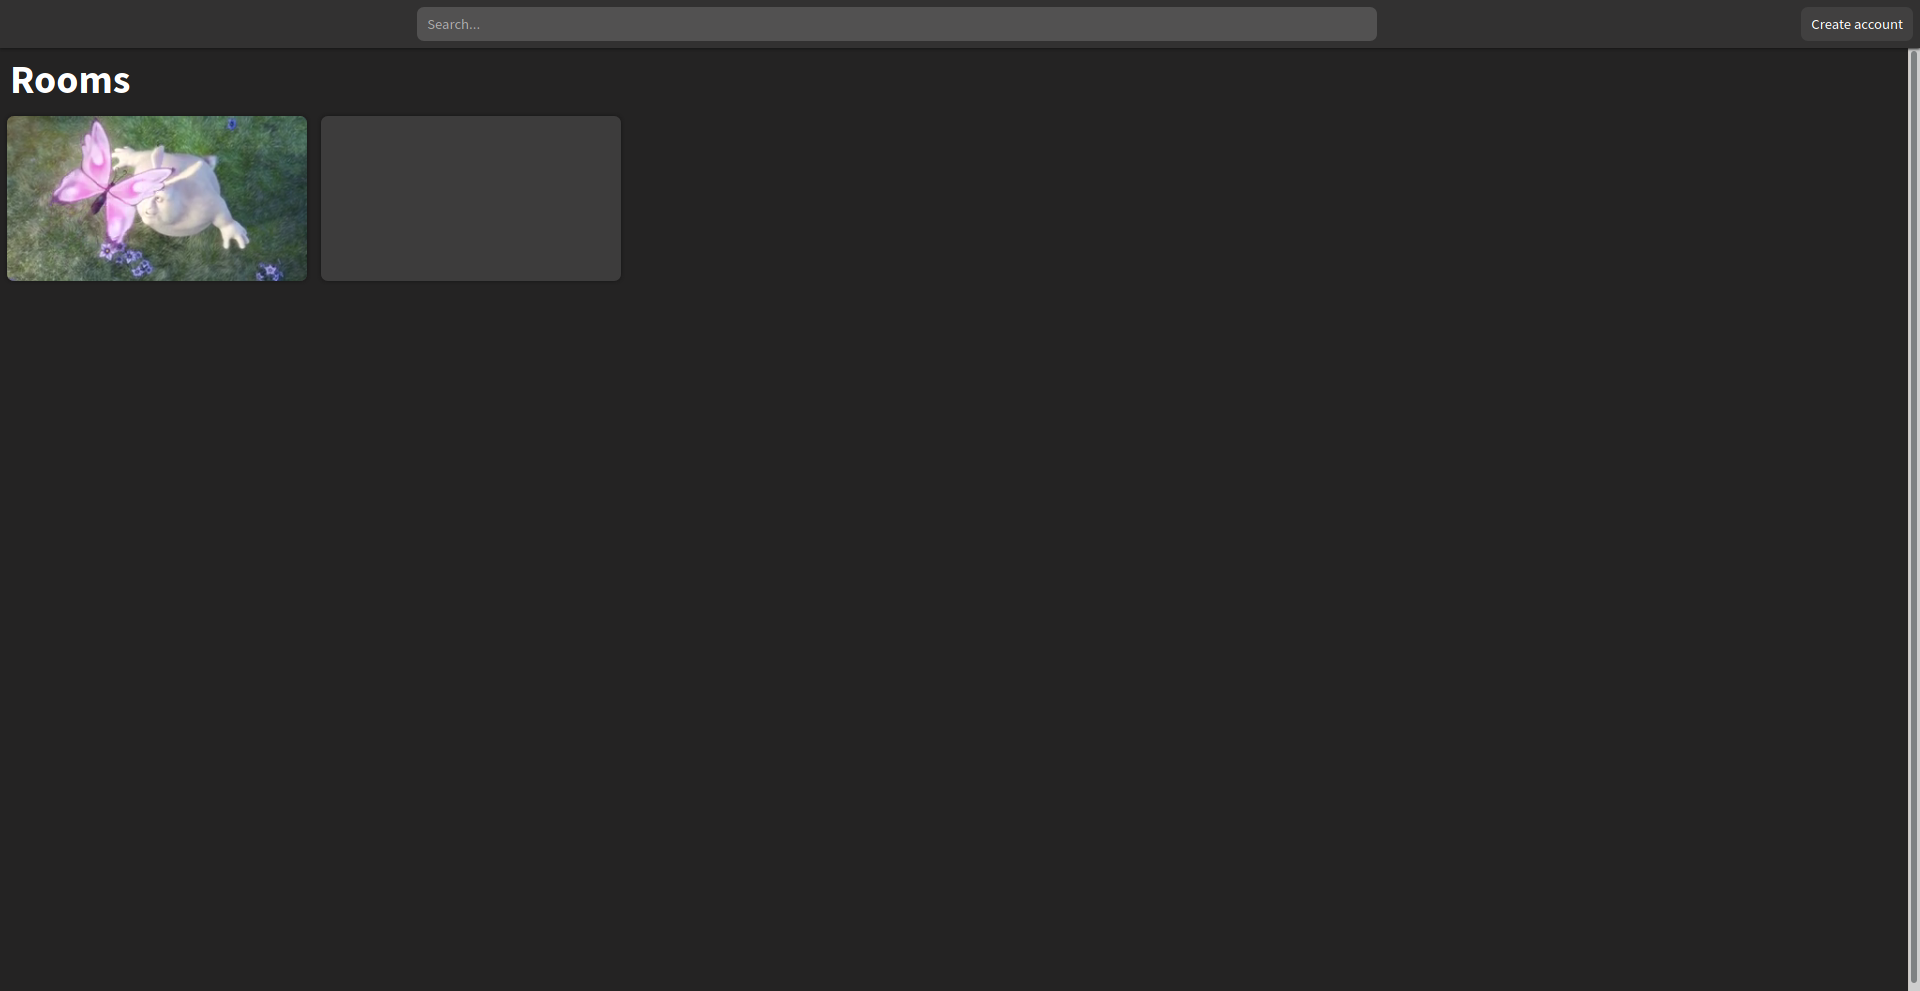
\includegraphics[scale=0.24]{main.png} 
%   \caption{Главная страница приложения}
%   \label{fig:arch:main_page}
%\end{figure}
% 
%\begin{figure}[H]
% \centering
%   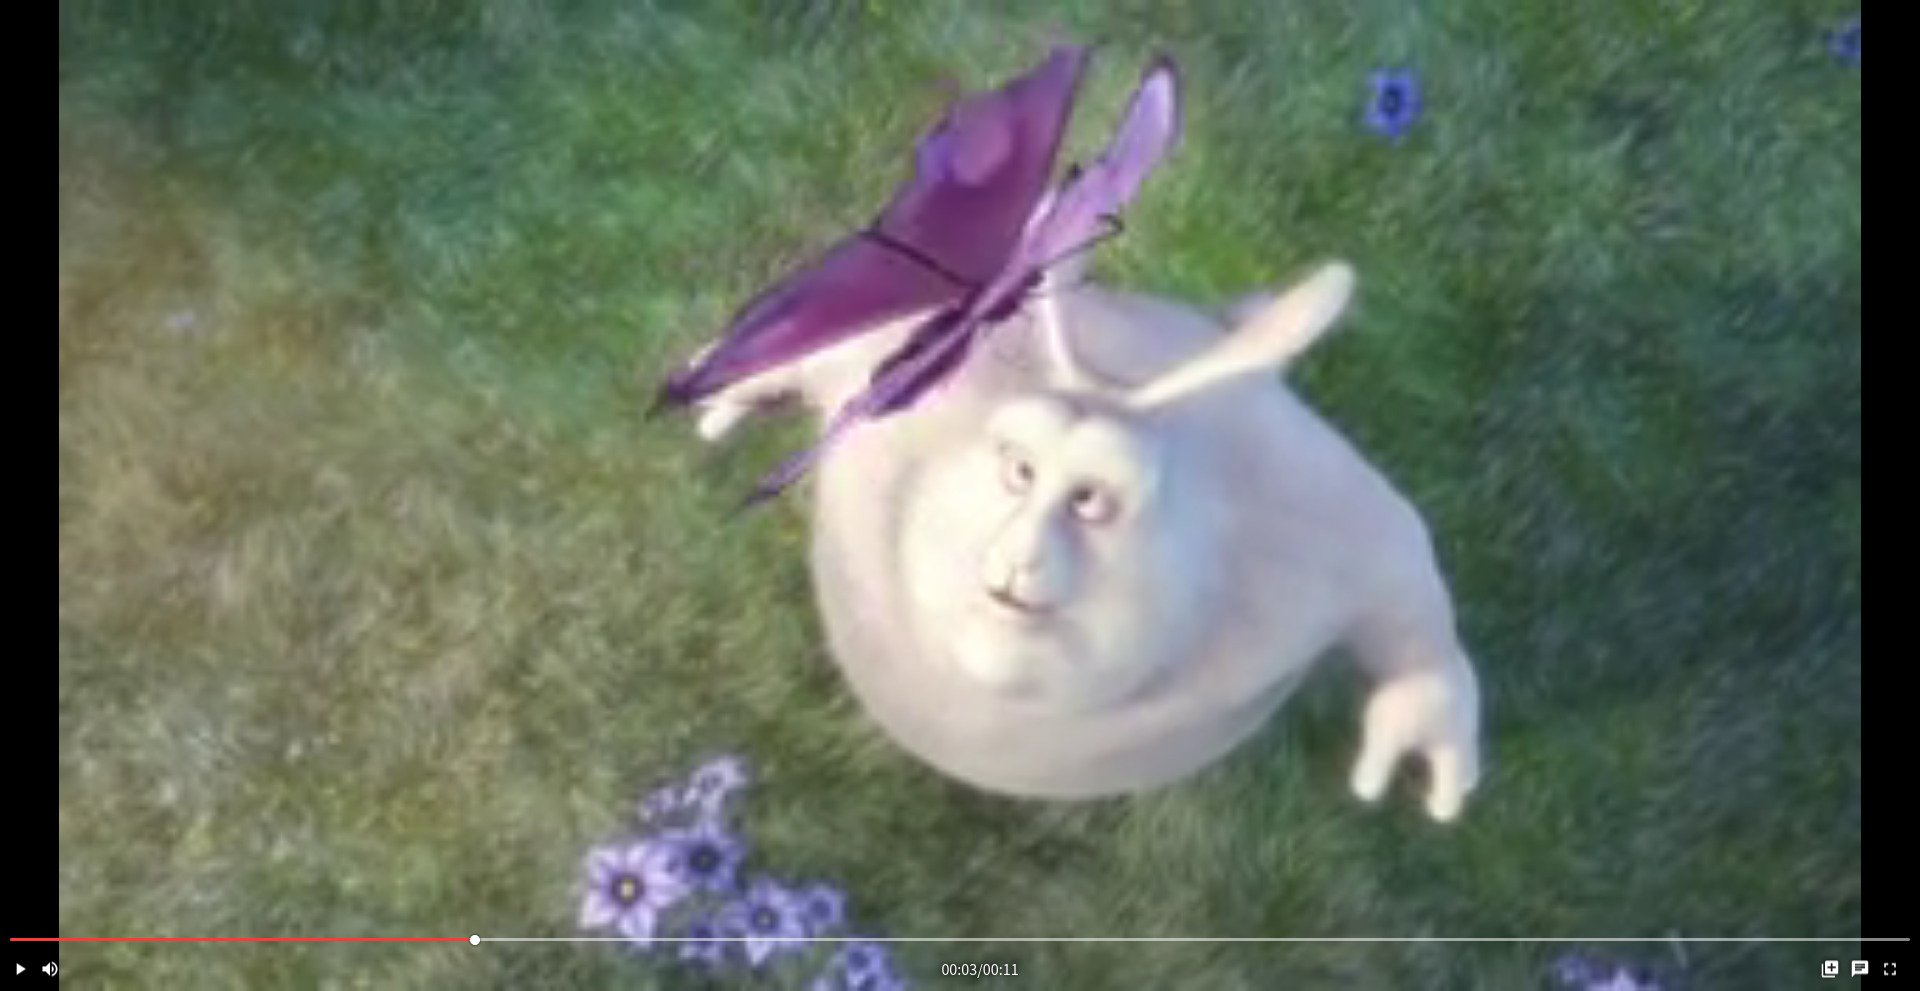
\includegraphics[scale=0.24]{room.jpg} 
%   \caption{Страница комнаты}
%   \label{fig:arch:room_page}
%\end{figure}
% 
%Основная страница содержит в себе следующий набор функциональных возможностей:
%\begin{itemize}
% \item авторизация пользователей;
% \item изменение пользовательских настроек;
% \item отображение доступных комнат;
% \item поиск комнат;
% \item предпросмотр комнат;
% \item переход на страницу комнаты.
%\end{itemize}
% 
%Станица плеера имеет следующие функции:
%\begin{itemize}
% \item проверка пароля комнаты;
% \item сохранение пароля при удачном вводе, чтобы пропустить его ввод в дальнейшем;
% \item воспроизведение видеоролика;
% \item остановка видеоролика;
% \item перемотка видеоролика;
% \item изменение громкости видеоролика;
% \item открытие видеоролика в полноэкранном режиме;
% \item отображение уведомлений о текущих действиях плеера;
% \item добавление видеоролика в список воспроизведения;
% \item добавление нескольких роликов в список воспроизведения;
% \item удаление ролика из списка воспроизведения;
% \item удаление всех роликов из списка воспроизведения;
% \item выбор следующего ролика для воспроизведения из списка воспроизведения;
% \item автоматическое включение следующего ролика из списка воспроизведения;
% \item синхронизация времени ролика между пользователями текущей комнаты;
% \item синхронизация состояния воспроизведения между пользователями текущей комнаты;
% \item синхронизация источника текущего видеоролика между пользователями текущей комнаты;
% \item отправка и получение сообщений в чате комнаты.
%\end{itemize}
% 
%\subsection{Учётная запись пользователя}
%Для работы пользователя с веб-приложением необходимо иметь учетную запись. Каждый пользователь при первом открытии страницы приложения автоматически получает учетную %запись без необходимости ввода каких-либо данных. Данная учетная запись имеет статус анонимной. Это сделано для того чтобы любой пользователь мог сразу начать %пользоваться сервисом. Пользователи с анонимной учетной записью имеют ряд ограничений:
%\begin{itemize}
% \item невозможно создать собственную комнату;
% \item невозможно сменить имя пользователя;
%\end{itemize}
% 
%Для того чтобы избавиться от ограничений пользователю необходимо создать собственную учетную запись. Для этого ему необходимо предоставить адрес электронной почты, %выбрать имя пользователя и пароль (для подтверждения пароля пользователь должен ввести его два раза). 
%В дальнейшем пользователь при посещении сайта будет сразу использовать созданную им учетную запись.
%Для сохранения пользовательской информации в рамках текущей сессии, она записывается в хранилище состояний, предоставленный JavaScript библиотекой Redux.
% 
%\subsection{Список комнат}
%Каждый пользователь имеет возможность просмотра списка комнат на главной странице. Данные для данного списка загружаются из базы данных и автоматически обновляются при %их изменении.
%Также пользователь имеет возможность производить поиск комнат, для этого имеется строка поиска в верхней части страницы.
% 
%Список комнат представлен в виде набора плиток. На данных плитках находится основная информация о данной комнате: название, защищённость паролем, а также окно %предпросмотра текущего видеоролика. 
%При нажатии на плитку комнаты пользователь перенаправляется на страницу данной комнаты. 
%
%\subsection{Комната}
%Перед тем как получить доступ к комнате происходит дополнительная проверка. 
%Если комната защищена паролем, то пользователь сначала попадает на страницу с формой для ввода пароля. 
%В случае ввода неправильного пароля пользователь получает уведомление об ошибке и ему предлагается ввести пароля снова. 
%При вводе верного пароля, он сохраняется в локальном хранилище браузера для повторного использования и пользователь получает доступ к комнате. 
%
%\subsection{Варианты использования}
%Далее будут рассмотрены основные варианты использования разработанного веб-приложения.
%
%\subsubsection{ВИ Создание учётной записи}~\par
%\label{use:reg}
%Описание ВИ: Пользователь имеет возможность при желании создать личную учётную запись.
% 
%Предусловия основного потока действий нет.
% 
%Основной поток действий:
%\begin{itemize}
%   \item пользователь нажимает кнопку "Create account";
%   \item пользователь вводит электронную почту, имя пользователя, пароль и подтверждение пароля.
%\end{itemize}
% 
%Ограничения: различные ограничения, установленные провайдером аутентификации Firebase.
% 
%\subsubsection{ВИ Использование своей учётной записи}~\par
%Описание ВИ: Пользователь имеет возможность использовать личную учётную запись.
% 
%Предусловия основного потока действий: у пользователя имеется учётная запись см.~\ref{use:reg}.
% 
%Основной поток действий:
%\begin{itemize}
%   \item пользователь нажимает кнопку "Create account";
%   \item пользователь нажимает кнопку "Existing user";
%   \item пользователь вводит электронную почту и пароль.
%\end{itemize}
% 
%Ограничения: различные ограничения, установленные провайдером аутентификации Firebase.
%
%\subsubsection{ВИ Создание комнаты}~\par
%\label{use:roomcreate}
%Описание ВИ: Пользователь имеет возможность создать комнату для совместного просмотра.
% 
%Предусловия основного потока действий: пользователь должен быть авторизован.
% 
%Основной поток действий:
%\begin{itemize}
%   \item пользователь нажимает кнопку "Create";
%   \item пользователь вводит название комнаты и пароль;
%   \item клиент получает список комнат и обновляет интерфейс.
%\end{itemize}
% 
%Ограничения: имя комнаты должно быть непустой строкой.
% 
%\subsubsection{ВИ Поиск комнаты}~\par
%Описание ВИ: Пользователь имеет возможность искать комнату по её имени для совместного просмотра.
% 
%Предусловия основного потока действий: Комната существует. Для создания комнаты см.~\ref{use:roomcreate}.
% 
%Основной поток действий:
%\begin{itemize}
%   \item пользователь начинает писать название комнаты;
%   \item при изменении текста в строке поиска система делает поиск по имени комнаты;
%   \item клиент получает список комнат и обновляет свой интерфейс.
%\end{itemize}
% 
%Ограничения: имя комнаты должно быть непустой строкой.
%
%\subsubsection{ВИ Подключение к комнате}~\par
%\label{use:join}
%Описание ВИ: Пользователь имеет возможность присоединиться к комнате для совместного просмотра.
% 
%Предусловия основного потока действий: комната должна существовать см.~\ref{use:roomcreate}.
% 
%Основной поток действий:
%\begin{itemize}
%   \item пользователь нажимает кнопку плитку комнаты из списка;
%   \item пользователь перенаправляется на страницу комнаты.
%\end{itemize}
% 
%Ограничения: при наличии у комнаты пароля пользователь должен ввести его, для подключения.
% 
%\subsubsection{ВИ Управление видеоплеером}~\par
%Описание ВИ: Пользователь имеет возможность управлять видеоплеером комнаты во время совместного просмотра.
% 
%Предусловия основного потока действий: комната должна существовать см.~\ref{use:roomcreate}, Пользователь присоединен к комнате см.~\ref{use:join}.
% 
%Основной поток действий:
%\begin{itemize}
%   \item Пользователь имеет следующие опций для управления плеером: запуск и остановка воспроизведения видео, перемотка, настройка громкости, открытие полноэкранного %режима.
%\end{itemize}
% 
%Ограничения: Для взаимодействия с плеером должно быть выбрано видео для воспроизведения см.~\ref{use:addvideo}.
% 
%\subsubsection{ВИ Добавление видео по ссылке}~\par
%\label{use:addvideo}
%Описание ВИ: Пользователь имеет возможность добавить видео в список воспроизведения комнаты для совместного просмотра.
% 
%Предусловия основного потока действий: комната должна существовать см.~\ref{use:roomcreate}, Пользователь присоединен к комнате см.~\ref{use:join}.
% 
%Основной поток действий:
%\begin{itemize}
%   \item пользователь открывает меню списка воспроизведения;
%   \item пользователь нажимает кнопку "Add";
%   \item пользователь вводит ссылку на ролик в строку поиска;
%   \item клиент получает список видео и обновляет интерфейс;
%   \item пользователь нажимает кнопку "Add" у нужного видеоролика.
%\end{itemize}
% 
%Ограничения: ссылка должна поддерживаться приложением.
% 
%\subsubsection{ВИ Удаление видео из списка воспроизведения}~\par
%Описание ВИ: Пользователь имеет возможность удалить видео в список воспроизведения комнаты для совместного просмотра.
% 
%Предусловия основного потока действий: комната должна существовать см.~\ref{use:roomcreate}, Пользователь присоединен к комнате см.~\ref{use:join}, в списке %воспроизведения должны быть видеоролики см.~\ref{use:addvideo}.
% 
%Основной поток действий:
%\begin{itemize}
%   \item пользователь открывает меню списка воспроизведения;
%   \item пользователь нажимает кнопку "крестик" у необходимого видеоролика.
%\end{itemize}
% 
%Альтернативный поток действий:
%\begin{itemize}
%   \item пользователь открывает меню списка воспроизведения;
%   \item пользователь нажимает кнопку "Reset".
%\end{itemize}
% 
%Ограничений нет.
% 
%\subsubsection{ВИ Использование чата}~\par
%Описание ВИ: Пользователь имеет возможность общаться с другими пользователями, используя текстовый чат.
% 
%Предусловия основного потока действий: комната должна существовать см.~\ref{use:roomcreate}, Пользователь присоединен к комнате см.~\ref{use:join}.
% 
%Основной поток действий:
%\begin{itemize}
%   \item пользователь открывает текстовый чат;
%   \item пользователь вводит сообщение в текстовое поле;
%   \item пользователь нажимает кнопку "Send" или клавишу Enter.
%\end{itemize}
% 
%Ограничения: сообщение должно быть непустой строкой.
%
%\subsection{Тестирование приложения}
% 
%Для проведения тестирования веб-приложения использовалось ПО из проекта Selenium. 
%В рамках данного проекта разработан набор различных программ, которые помогают автоматизировать процесс тестирования веб-приложений. 
%Для данного проекта использовался Selenium WebDriver - универсальный интерфейс для взаимодействия с драйвером браузера, веб-браузер Firefox и драйвер geckodriver. 
%Для проведения тестов использовалась библиотека для языка Python и расширение для браузера Firefox~--- Selenium IDE.
% 
%Также было проведено ручное тестирование механизма синхронизации, так как при помощи Selenium их протестировать затруднительно. 
%В рамках ручного тестирования было проведено дымовое тестирование возможностей видеоплеера и механизмов синхронизации.
%

% \newcommand{\companyname}{\mbox{<<Техартгруп>>}}

\section{Охрана труда}

\subsection[Обеспечение пожарной безопасности на предприятии]{Обеспечение пожарной безопасности на предприятии малого бизнеса \companyname{}}


Целью дипломного проекта является реализация и анализ алгоритмов построения вероятностных сетей.
Вероятностная сеть является компактным и эффективным способом представления знаний.
Вероятностные сети используются в программном обеспечении для принятия решения в условиях недостаточной определенности.
Данный способ статистического моделирования показал свою пригодность в реальных условиях в сложных предметных областях: медицине, космической промышленности, финансовой сфере и других областях.
Первоначальные стадии разработки дипломного проекта выполнялись на предприятии ООО~\companyname{} во время прохождения преддипломной практики.
В настоящем разделе рассматриваются вопросы, связанные с обеспечением пожарной безопасности на предприятии.

Предприятие \companyname{} занимается предоставлением услуг по разработке информационных систем для иностранных предприятий. 
В минском офисе компании на данный момент работает более 200 человек. 
% TODO: Переписать абсолютный бред в оставшейся части абзаца.
Большое количество конкурирующих компаний, разрабатывающих программное обеспечение в Минске, способствует повышению общего уровня условий труда.
Это, в частности, сказывается на комфортабельности рабочих мест.
Работникам предоставляются светлые, проветриваемые, тихие кабинеты, гибкий график рабочего времени, специальные комнаты отдыха и т.\,д.
Современные компании негласно ориентируются на соответствие лучшим мировым практикам в области охраны труда и, в частности, пожарной безопасности.

На предприятии \companyname{} за пожарную безопасность отвечает директор компании.
Для каждого нового сотрудника производится инструктаж по пожарной безопасности и технике безопасности, а так же знакомство с планом эвакуации при возникновении черезвычайных ситуаций~\cite[\ignore{раздел~5.5.8,} с.~324]{michnuk_2009}.
За проведение инструктажа отвечает специальный человек из отдела материально"=технического снабжения предприятия.
В компании действует набор правил, обязательных для исполнения сотрудниками.
В целях повышения пожарной безопасности курение в здании офиса запрещено.
Все сотрудники обязаны в конце рабочего дня выключить свои персональные компьютеры и обесточить их.
В конце рабочего дня специальный сотрудник проверяет соблюдение данного правила в каждом рабочем кабинете, чтобы там были выключены все электрические приборы: компьютеры, электрические чайники, кондиционеры, освещение и т.\,д.
Все рабочие компьютеры подключены к источникам бесперебойного питания, которые подключены к сетевыми фильтрам, защищающим от скачков напряжения в электросети.

Офис компании расположен в центре города.
Здание офиса представляет собой монолитную железобетонную конструкцию высотой шесть этажей, офис компании находится на двух верхних этажах.
Конструкция здания предусматривает три способа эвакуации с этажа: выход в паркинг, лестничная клетка с выходом на улицу, лестничная клетка с выходом на первый этаж паркинга. 
В случае недоступности основных эвакуационных выходов из каждого кабинета можно через окно попасть на лоджию~\cite[\ignore{раздел~5.5.4,} с.~314\,--\,316]{michnuk_2009}.
Схемы эвакуации выдаются в виде электронного документа каждому новому сотруднику, а также находятся на специальном стенде в рабочих кабинетах.
Все кабинеты офиса расположены вдоль длинного коридора, который оборудован специальными аварийными светильниками и знаками, указывающими направление эвакуации.
На случай отключения электроэнергии компания имеет два дизельных"=генератора, обеспечивающих нужды предприятия на случай отключения электроэнергии.

Офис компании оборудован необходимыми средствами сигнализации о пожаре~\cite[с.~215]{sinilov_2010}. %\cite[с.~5\,--\,7]{sharovar_1979}. 
Каждый кабинет оборудован пожарным дымовым оптико"=электрическим точечным извещателем \mbox{ИП212-02М1} (рисунок~\ref{fig:fire_alarms}).
На предприятии производиться регулярный контроль и проверка работоспособности пожарных извещателей специальным человеком из отдела материально"=технического снабжения предприятия.
В коридорах дополнительно установлены ручные пожарные извещатели \mbox{ИП 5-2Р} (рисунок~\ref{fig:fire_alarms}).
Для извещения о пожаре также может быть использована корпоративная электронная почта, а также другие современные способы обмена информацией.

\begin{figure}[ht]
\centering
  \begin{subfigure}[b]{0.45\textwidth} 
    \centering
    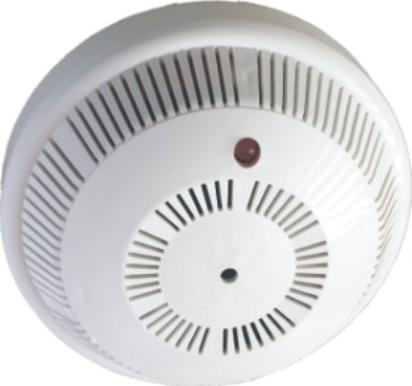
\includegraphics[scale=0.85]{avt_pozh_izv.jpg}  
    \caption{}
  \end{subfigure}
  \begin{subfigure}[b]{0.45\textwidth} 
    \centering
    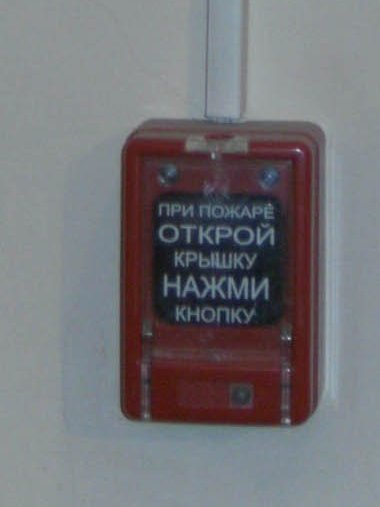
\includegraphics[scale=1.2]{ruch_pozh_izv.jpg}  
    \caption{}
  \end{subfigure}
  \caption{ а "--- автономный пожарный извещатель;
            б "--- ручной пожарный извещатель.}
  \label{fig:fire_alarms}
\end{figure}

На случай возникновения пожара в каждом рабочем кабинете находиться ручной порошковый огнетушитель \mbox{ОП-10}~(з)~МИГ~М (рисунок~\ref{fig:extinguishing_fire}), пригодный для тушения пожаров различного типа, в том числе для тушения электрических приборов~\cite[\ignore{раздел 5.5.7,} с.~221\,--\,323]{michnuk_2009}.
Каждый этаж здания офиса оборудован двумя пожарными кранами для тушения пожара.
Пожарные краны расположены в противоположных частях коридора, недалеко от эвакуационных выходов (рисунок~\ref{fig:extinguishing_fire}).
На случай воспламенения электрической проводки или другого электрического оборудования в каждом кабинете установлены электрические щитки, необходимые для отключения подачи электроэнергии в пределах кабинета.
Во всех помещениях офиса предприятия установлена оросительная система пожаротушения для ликвидации возгорания до приезда пожарной службы~\cite[\ignore{раздел~5.5.6,} с.~318\,--\,320]{michnuk_2009}.
При расследовании возможных причин возникновения пожара может быть задействована система видео"=наблюдения, установленная во всех помещениях предприятия.

\begin{figure}[ht]
\centering
  \begin{subfigure}[b]{0.45\textwidth} 
    \centering
    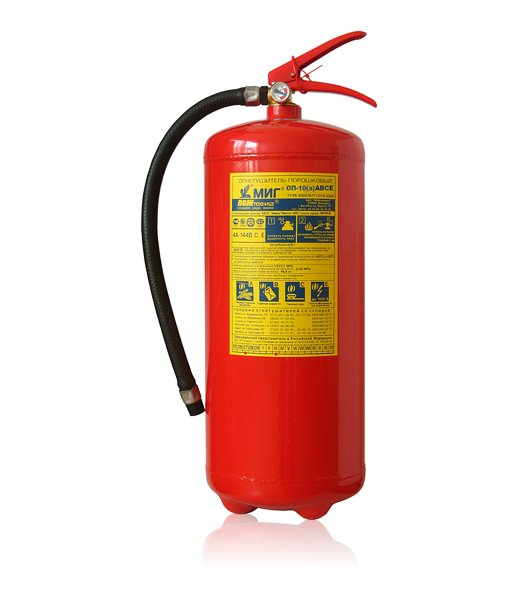
\includegraphics[scale=0.34]{ognetush.jpg}  
    \caption{}
  \end{subfigure}
  \begin{subfigure}[b]{0.45\textwidth} 
    \centering
    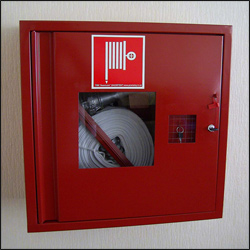
\includegraphics[scale=0.7]{pozh_kran.jpg}  
    \caption{}
  \end{subfigure}
  \caption{ а "--- порошковый огнетушитель \mbox{ОП-10}~(з)~МИГ~М;
            б "--- пожарный кран.}
  \label{fig:extinguishing_fire}
\end{figure}

Основной род деятельности на предприятии "--- разработка информационных систем "--- не предусматривает непосредственный контакт с горючими или легко"=воспламеняющимися веществами, что сильно снижает риски возникновения пожара на предприятии.
Наиболее вероятными причинами возникновения пожара, с учетом специфики предприятия, могут являться нарушение правил внутреннего распорядка "--- курение на рабочем месте, и неисправность электрического оборудования, которого в офисе компании достаточно~\cite[\ignore{раздел 5.5.1,} с.~312]{michnuk_2009}.
С целью снижения риска возникновения пожара по причине неисправности электрического оборудования в компании запрещено пользоваться неисправным оборудованием, а все исправное оборудование подключается в сеть через специальные сетевые фильтры и источники бесперебойного питания.
В целом правила распорядка на предприятии и высокая культура работы с электрическим оборудованием снижают риски возникновения пожара до минимума.

Большой проблемой в достижении максимальной пожарной безопасности предприятия является доступность подъезда пожарной техники к зданию офиса.
В будние дни прилегающие улицы, стоянки, пешеходные переходы заняты неправильно припаркованным личным транспортом.
Большую часть светлого времени суток движение по прилегающим улицам очень затруднено.
Данную проблему предприятие не в силах решить самостоятельно, проблема заключается в низкой культуре владельцев транспорта и игнорировании многочисленных нарушений правил дорожного движения  сотрудниками ГАИ.
% Заключительное предложение
Таким образом, изложенные выше предложения, не смотря на проблемы с подъездом пожарной техники, обеспечат пожарную безопасность на предприятии \companyname{}.


% \include{sec_test}

\newcommand{\byr}{Br}
\section{Технико-экономическое обоснование}
 
\subsection{Описание функций, назначения и потенциальных пользователей ПО}
Разрабатываемое в дипломном проекте мобильное приложение предназначено для упрощения поиска по множеству игровых магазинов с функциями просмотра сохранённых предложений и скидок, подсчёта статистики и возможной выгоде при покупке определённой игры.
 
Основными функциями разрабатываемого мобильного приложения являются:
\begin{itemize}
 \item возможность использовать мобильное приложение неавторизованным пользователям;
 \item возможность регистрации профиля для доступа к дополнительным функциям;
 \item фильтрация поиска по множеству магазинов;
 \item поиск игр по их атрибутам: названию, идентификационному номеру;
 \item поиск скидок по их атрибутам: идентификационному номеру, цене, рейтингу, названию игры, на скидке ли она;
 \item возможность добавить предложение или игру в список избранного;
 \item просмотру дополнительной информации об игре: рейтинг в сервисе Steam, баллы Metacritic, отзывы;
 \item регистрация и синхронизация настроек через сторонние сервисы.
\end{itemize}
 
Функции приложения предусматривают использование базы данных для кеширования данных пользователя, информации о загруженных магазинах и их предложений, а также настроек пользователя.
 
В качестве основного языка программирования был выбран Kotlin вместе с Android SDK для создания клиентской части. В качестве стороннего сервиса авторизации и удаленной базы данных был выбран Google Firebase.
 
Разрабатываемый программный продукт создан для пользователей, которые из-за пандемии, отсутствии денег, вынуждены экономить на покупке игр. Приложение позволяет сэкономить на покупке лицензионных версий игр путем агрегации всех популярных магазинов и удобному поиску по их скидкам.

Программный продукт разработан для получения прибыли от свободной реализации на рынке IT, следовательно, экономический эффект достигается за счет получения прибыли от его продажи множеству потребителей. Фримиум выбрана в качестве основной модели монетезации. Пользователь имеет бесплатный доступ к ограниченному функционалу приложения, после переходит на платный вариант по подписке.

Основными функциями платной версии мобильного приложения являются:
\begin{itemize}
 \item большее количество возможностей для поиска;
 \item неограниченный по размерности список избранного;
 \item дополнительные магазины с уникальными для этих магазинов функциями.
\end{itemize}
 
\subsection{Расчет затрат на разработку ПО}
 
Для разработки данного мобильного приложения необходимы следующие специалисты: ведущий программист, программист, дизайнер и тестировщик. Трудоёмкость работ, вид работ и ставки  представлены в таблице~\ref{table:econ:initial_data}.
 

Затраты на основную заработную плату команды.
Расчет основной заработной платы каждого из команды осуществляется по формуле:
\hfill \break
\begin{equation}
 \label{eq:econ:payment}
 \text{З}_\text{О} = \sum_{i = 1}^{n}  \text{З}_{чi} \cdot t_{i} \text{\,,}
\end{equation}
\hfill \break
\begin{explanation}
где & $ n $ & количество исполнителей, занятых разработкой конкретного ПО; \\
   & $ \text{З}_{чi} $ & часовая заработная плата i-го исполнителя (р.); \\
   & $ t_{i} $ & трудоемкость работ, выполняемых i-м исполнителем (ч).
\end{explanation}
 
\begin{table}[!ht]
\caption{Расчет затрат на основную заработную плату команды}
\label{table:econ:initial_data}
 \centering
 \begin{tabular}
 {| >{\raggedright}m{0.02\textwidth}
 | >{\centering}m{0.18\textwidth}
 | >{\centering}m{0.18\textwidth}
 | >{\centering}m{0.13\textwidth}
 | >{\centering}m{0.18\textwidth}
 | >{\centering\arraybackslash}m{0.15\textwidth}|}
   \hline
   № & Участник команды & Вид выполняемой работы & Часовая тарифная ставка, р. & Трудоемкость работ, ч & Зарплата по тарифу, p.\\
   \hline
   1 & 2 & 3 & 4 & 5 & 6 \\
 
   \hline
   1 & Ведущий программист & Руководство, разработка архитектуры приложения, поддержание стабильности исходного кода & 7,61 & 672 & 5113,92 \\
 
   \hline
   2 & Программист & Разработка функционала, написание тестов, поддержка исходного кода & 5,67 & 672 & 3810,24 \\
 
   \hline
   3 & Дизайнер & Разработка UI/UX & 3,47 & 168 & 582,96 \\
 
   \hline
   4 & Тестировщик & Написание автотестов, тестирование, сверка требований & 4,45 & 504 & 2242,8 \\
 
   \hline
   \multicolumn{5}{|c|}{Итого затраты на основную заработную плату разработчиков} & 11749,92\\
  
   \hline
 \end{tabular}
\end{table}

Затраты на дополнительную заработную плату команды разработчиков определяется по формуле:
\hfill \break
\begin{equation}
 \label{eq:econ:add_payment}
 \text{З}_\text{Д} = \frac{ \text{З}_\text{О} \cdot \text{H}_\text{Д}}
 {\num{100\%}}  \text{\,,}
\end{equation}
\hfill \break
\begin{explanation}
где & $ \text{З}_\text{О} $ & затраты на основную заработную плату, (р.); \\
   & $ \text{З}_{чi} $ & норматив дополнительной заработной платы, \% (НД = 40\%).
\end{explanation}
\begin{equation}
 \label{eq:econ:add_payment_calc}
 \text{З}_\text{Д} = \frac{ 11749,92 \cdot 40}{100} = 4699,97 \text{ р.}
\end{equation}
\hfill \break
Отчисления на социальные нужды (в фонд социальной защиты населения и на обязательное страхование) определяются в соответствии с действующими законодательными актами по формуле: 
\hfill \break
\begin{equation}
 \label{eq:econ:add_payment}
 \text{P}_\text{СОЦ} = \frac{ (\text{З}_\text{О}+\text{З}_\text{Д}) \cdot \text{H}_\text{СОЦ}}{\num{100}}  \text{\,,}
\end{equation}
\hfill \break
\begin{explanation}
где & $ \text{H}_\text{СОЦ} $ & норматив отчислений на социальные нужды, \% (НСОЦ = 35\%). \\
\end{explanation}
\begin{equation}
 \label{eq:econ:add_payment}
 \text{P}_\text{СОЦ} = \frac{ (11749,92 + 4699,97) \cdot 35}{\num{100}} = 5757,46 \text{ р.}
\end{equation}
\hfill \break
Прочие затраты включаются в себестоимость разработки ПО в процентах от затрат на основную заработную плату команды разработчиков по формуле:
\hfill \break
\begin{equation}
 \label{eq:econ:add_payment}
 \text{З}_\text{ПЗ} = \frac{ \text{З}_\text{О} \cdot \text{H}_\text{ПЗ}}{\num{100}}  \text{\,,}
\end{equation}
\hfill \break
\begin{explanation}
где & $ \text{H}_\text{ПЗ} $ & норматив прочих затрат, \% (НПЗ = 150\%).
\end{explanation}
\begin{equation}
 \label{eq:econ:add_payment}
 \text{З}_\text{ПЗ} = \frac{ 11749,92 \cdot 150}{\num{100}} = 17624,88 \text{ р.}
\end{equation}
\hfill \break
Полная сумма затрат на разработку программного обеспечения находится путем суммирования всех рассчитанных статей затрат. Итоговые данные представлены в таблице~\ref{table:econ:total_price}.
 
\begin{table}[!ht]
\caption{Затраты на разработку программного обеспечения}
\label{table:econ:total_price}
 \centering
 \begin{tabular}{| >{\raggedright}m{0.62\textwidth}
                 | >{\centering\arraybackslash}m{0.33\textwidth}|}
   \hline
   \begin{center}
     Статья затрат
   \end{center} & Сумма, р.\\
   \hline
   Основная заработная плата команды разработчиков & 11749,92\\
 
   \hline
   Дополнительная заработная плата команды разработчиков & 4699,97\\
 
   \hline
   Отчисления на социальные нужды & 5757,46\\
 
   \hline
   Прочие затраты & 17624,88\\
 
   \hline
   \textbf{Общая сумма затрат на разработку} & 39832,23\\
   \hline
 
 \end{tabular}
\end{table}
 
Общая сумма затрат на разработку мобильного приложения составит\linebreak39832,23 рублей.
 
\subsection{Экономический эффект при разработке ПО}
Экономический эффект организации-разработчика программного обеспечения в данном случае представляет собой прибыль (чистая прибыль) от его продажи множеству потребителей. Прибыль рассчитывается по формулам:
 
\hfill \break
\begin{equation}
 \label{eq:econ:add_payment}
 \text{П}_\text{Ч} = \text{П} - \frac{ \text{П} \cdot \text{H}_\text{П}}{\num{100}}  \text{\,,}
\end{equation}
 
\begin{equation}
 \label{eq:econ:add_payment}
 \text{П} = \text{Ц} \cdot N - \text{НДС} - \text{З}_\text{Р}  \text{\,,}
\end{equation}
 
\begin{equation}
 \label{eq:econ:add_payment}
 \text{НДС} = \frac{ \text{Ц} \cdot N \cdot \text{Н}_\text{ДС}} {\num{100\%} + \text{Н}_\text{ДС}}.
\end{equation}
\linebreak
\linebreak
\begin{explanation}
 где & $ \text{Ц} $ & цена реализации ПО заказчику (р.); \\
 & $ \text{НДС} $ & сумма налога на добавленную стоимость (р.); \\
 & $ \text{Н}_\text{ДС} $ & ставка налога на добавленную стоимость согласно действующему законодательству, \% (Ндс = 20 \%); \\
 & $ \text{H}_\text{П} $ & ставка налога на прибыль, \% (Нп =18 \%); \\
 & $ \text{З}_\text{Р} $ & Общая сумма затрат на разработку мобильного приложения(р.).
\end{explanation}
 
Приложение будет иметь закрытый функционал за подпиской, следовательно стабильный доход планируется получать с продажи пользователям подписки. Стоимость подписки 19,81 р. в месяц. Беря во внимание пандемию и подъем игровой индустрии, пессимистичный исход по количеству подписок будет равно 250 человек.
\linebreak
\linebreak
\begin{equation}
 \label{eq:econ:add_payment}
 \text{НДС} = \frac{ 19,81 \cdot 250 \cdot 0,2} {1,2} = 825,42 {\text{ р.}}
\end{equation}
 
\begin{equation}
 \label{eq:econ:add_payment}
 \text{П} = (19,81 \cdot 12) \cdot 250 - 825,42 - 39832,23 = 18772,35 {\text{ р.}} 
\end{equation}
 
\begin{equation}
 \label{eq:econ:add_payment}
 \text{П}_\text{Ч} =  18772,35 - (  18772,35 \cdot 18 )/100 = 15393,327 \text{ р.}
\end{equation}
\linebreak
\linebreak
При пессимистичном прогнозе чистая прибыль составила 15393,327 рублей. Уровень рентабельности вычислим по формуле:
\linebreak
\linebreak
\begin{equation}
 \label{eq:econ:add_payment}
 \text{У}_\text{Р} = \frac{\text{П}_\text{Ч}}{\text{З}_\text{Р}} \cdot 100\%  \text{\,,}
\end{equation}
 
\begin{equation}
 \label{eq:econ:add_payment}
 \text{У}_\text{Р} = \frac{15393,327}{39832,23} \cdot 100\% = 38\%.
\end{equation}
\linebreak
\linebreak
При рассчетах уровень рентабельности оказался равен 38 \% с условием реализации приложения в течении одного года. Данное значение выше 13 \% процентной ставки по банковским депозитам, следовательно разработка мобильного приложения является оправданной.
\linebreak
\linebreak
\begin{equation}
 \label{eq:econ:add_payment}
 \text{Т}_\text{ОК} = \frac{39832,23}{15393,327} = 2,6  \text{ года.}
\end{equation}
\linebreak
\linebreak
При пессимистичных прогнозах, без падения прибыли из-за непредвиденных ситуаций, разработка мобильного приложения окупиться на третий год реализации.
 
\subsection{Заключение}
В результате работы по технико-экономическому обоснованию разработки агрегатора игровых магазинов были вычислены затраты на общую разработку, предполагаемую прибыль, рентабельность затрат и срок окупаемости:
\begin{itemize}
 \item затраты на разработку составляют 39832,23 рублей;
 \item пессимистический уровень чистой годовой прибыли составляет\linebreak15393,327 рублей;
 \item уровень рентабельности затрат на разработку равен 38 \%;
 \item окупаемость разработки в течении 3 лет.
\end{itemize}
 Конечные данные обозначают оправданность разработки мобильного приложения. Стоит заметить, что расчёты были выполнены с учетом сложившейся в мире обстановки глобальной пандемии и огромного роста рынка игровой индустрии в следствии карантина и глобальной изоляции. В данный момент на рынке существует множество предложений от разных игровых магазинов, разделение аудитории между игровыми магазинами является одной из самых важных проблем в игровой индустрии. Пользовательская база разделяется между магазинами, что влечёт ситуацию в которой пользователи просто не успевают следить за всеми магазинами которые предлагает рынок. В первую очередь данное приложение решает вопрос со сбором всех магазинов в одном месте и предоставлении пользователю удобный интерфейс по отслеживанию лучших скидок на рынке. Дополнительные функции в виде поиска отдельных игр и их фильтрации, а также ранжировании разных интересных предложений на главной странице приложения решает основные вопросы возникающие на таком быстроразвивающемся рынке как игровая индустрия. В последнюю очередь социальные функции и встроенная аналитика в приложение поможет определить магазины которые наиболее интересны пользователям, что позволит провести переоценку магазинов и принимать решения о перенастройке ранжирования в пользу этих магазинов для увеличения популярности и рентабельности приложения на рынке. В будущем можно говорить о заключении персональных контрактов с магазинами и их специальном ранжировании и интеграции в приложение. Дополнительно можно добавить возможность добавления специальных рекламных страниц для каждой из игр и рекомендации таких игр пользователям по просьбе сторонних игровых студий. В конечном итоге данное мобильное приложение и его сфера деятельности открывают много возможностей для развития в экономическом плане и множество точек роста.
 

% % Begin Calculations

% \FPeval{\totalProgramSize}{15680}
% \FPeval{\totalProgramSizeCorrected}{8650}

% \FPeval{\normativeManDays}{224}

% \FPeval{\additionalComplexity}{0.12}
% \FPeval{\complexityFactor}{clip(1 + \additionalComplexity)}

% \FPeval{\stdModuleUsageFactor}{0.7}
% \FPeval{\originalityFactor}{0.7}

% \FPeval{\adjustedManDaysExact}{clip( \normativeManDays * \complexityFactor * \stdModuleUsageFactor * \originalityFactor )}
% \FPround{\adjustedManDays}{\adjustedManDaysExact}{0}

% \FPeval{\daysInYear}{365}
% \FPeval{\redLettersDaysInYear}{9}
% \FPeval{\weekendDaysInYear}{104}
% \FPeval{\vocationDaysInYear}{21}
% \FPeval{\workingDaysInYear}{ clip( \daysInYear - \redLettersDaysInYear - \weekendDaysInYear - \vocationDaysInYear ) }

% \FPeval{\developmentTimeMonths}{3}
% \FPeval{\developmentTimeYearsExact}{clip(\developmentTimeMonths / 12)}
% \FPround{\developmentTimeYears}{\developmentTimeYearsExact}{2}
% \FPeval{\requiredNumberOfProgrammersExact}{ clip( \adjustedManDays / (\developmentTimeYears * \workingDaysInYear) + 0.5 ) }

% % тут должно получаться 2 ))
% \FPtrunc{\requiredNumberOfProgrammers}{\requiredNumberOfProgrammersExact}{0}

% \FPeval{\tariffRateFirst}{600000}
% \FPeval{\tariffFactorFst}{3.04}
% \FPeval{\tariffFactorSnd}{3.48}


% \FPeval{\employmentFstExact}{clip( \adjustedManDays / \requiredNumberOfProgrammers )}
% \FPtrunc{\employmentFst}{\employmentFstExact}{0}

% \FPeval{\employmentSnd}{clip(\adjustedManDays - \employmentFst)}


% \FPeval{\workingHoursInMonth}{160}
% \FPeval{\salaryPerHourFstExact}{clip( \tariffRateFirst * \tariffFactorFst / \workingHoursInMonth )}
% \FPeval{\salaryPerHourSndExact}{clip( \tariffRateFirst * \tariffFactorSnd / \workingHoursInMonth )}
% \FPround{\salaryPerHourFst}{\salaryPerHourFstExact}{0}
% \FPround{\salaryPerHourSnd}{\salaryPerHourSndExact}{0}

% \FPeval{\bonusRate}{1.5}
% \FPeval{\workingHoursInDay}{8}
% \FPeval{\totalSalaryExact}{clip( \workingHoursInDay * \bonusRate * ( \salaryPerHourFst * \employmentFst + \salaryPerHourSnd * \employmentSnd ) )}
% \FPround{\totalSalary}{\totalSalaryExact}{0}

% \FPeval{\additionalSalaryNormative}{20}

% \FPeval{\additionalSalaryExact}{clip( \totalSalary * \additionalSalaryNormative / 100 )}
% \FPround{\additionalSalary}{\additionalSalaryExact}{0}

% \FPeval{\socialNeedsNormative}{0.5}
% \FPeval{\socialProtectionNormative}{34}
% \FPeval{\socialProtectionFund}{ clip(\socialNeedsNormative + \socialProtectionNormative) }

% \FPeval{\socialProtectionCostExact}{clip( (\totalSalary + \additionalSalary) * \socialProtectionFund / 100 )}
% \FPround{\socialProtectionCost}{\socialProtectionCostExact}{0}

% \FPeval{\taxWorkProtNormative}{4}
% \FPeval{\taxWorkProtCostExact}{clip( (\totalSalary + \additionalSalary) * \taxWorkProtNormative / 100 )}
% \FPround{\taxWorkProtCost}{\taxWorkProtCostExact}{0}
% \FPeval{\taxWorkProtCost}{0} % это считать не нужно, зануляем чтобы не менять формулы

% \FPeval{\stuffNormative}{3}
% \FPeval{\stuffCostExact}{clip( \totalSalary * \stuffNormative / 100 )}
% \FPeval{\stuffCost}{\stuffCostExact}

% \FPeval{\timeToDebugCodeNormative}{15}
% \FPeval{\reducingTimeToDebugFactor}{0.3}
% \FPeval{\adjustedTimeToDebugCodeNormative}{ clip( \timeToDebugCodeNormative * \reducingTimeToDebugFactor ) }

% \FPeval{\oneHourMachineTimeCost}{5000}

% \FPeval{\machineTimeCostExact}{ clip( \oneHourMachineTimeCost * \totalProgramSizeCorrected / 100 * \adjustedTimeToDebugCodeNormative ) }
% \FPround{\machineTimeCost}{\machineTimeCostExact}{0}

% \FPeval{\businessTripNormative}{15}
% \FPeval{\businessTripCostExact}{ clip( \totalSalary * \businessTripNormative / 100 ) }
% \FPround{\businessTripCost}{\businessTripCostExact}{0}

% \FPeval{\otherCostNormative}{20}
% \FPeval{\otherCostExact}{clip( \totalSalary * \otherCostNormative / 100 )}
% \FPround{\otherCost}{\otherCostExact}{0}

% \FPeval{\overheadCostNormative}{100}
% \FPeval{\overallCostExact}{clip( \totalSalary * \overheadCostNormative / 100 )}
% \FPround{\overheadCost}{\overallCostExact}{0}

% \FPeval{\overallCost}{clip( \totalSalary + \additionalSalary + \socialProtectionCost + \taxWorkProtCost + \stuffCost + \machineTimeCost + \businessTripCost + \otherCost + \overheadCost ) }

% \FPeval{\supportNormative}{30}
% \FPeval{\softwareSupportCostExact}{clip( \overallCost * \supportNormative / 100 )}
% \FPround{\softwareSupportCost}{\softwareSupportCostExact}{0}


% \FPeval{\baseCost}{ clip( \overallCost + \softwareSupportCost ) }

% \FPeval{\profitability}{35}
% \FPeval{\incomeExact}{clip( \baseCost / 100 * \profitability )}
% \FPround{\income}{\incomeExact}{0}

% \FPeval{\estimatedPrice}{clip( \income + \baseCost )}

% \FPeval{\localRepubTaxNormative}{3.9}
% \FPeval{\localRepubTaxExact}{clip( \estimatedPrice * \localRepubTaxNormative / (100 - \localRepubTaxNormative) )}
% \FPround{\localRepubTax}{\localRepubTaxExact}{0}
% \FPeval{\localRepubTax}{0}

% \FPeval{\ndsNormative}{20}
% \FPeval{\ndsExact}{clip( (\estimatedPrice + \localRepubTax) / 100 * \ndsNormative )}
% \FPround{\nds}{\ndsExact}{0}


% \FPeval{\sellingPrice}{clip( \estimatedPrice + \localRepubTax + \nds )}

% \FPeval{\taxForIncome}{18}
% \FPeval{\incomeWithTaxes}{clip(\income * (1 - \taxForIncome / 100))}
% \FPround\incomeWithTaxes{\incomeWithTaxes}{0}

% % End Calculations

% Целью дипломного проекта является разработка и анализ алгоритмов построения вероятностных сетей.
% Вероятностные сети используются в ПО для принятия решения в условиях недостаточной определенности.
% Данный способ статистического моделирования показал свою пригодность в реальных условиях в сложных предметных областях: медицине, космической промышленности, финансовой сфере и других областях.
% Для достижения указанной цели планируется разработать ПО для представления и синтеза вероятностных сетей. 
% Сеть синтезируется по набору данных и позволяет производить оценку параметров распределения случайных величин, характеризующих неизвестные данные. 

% \subsection{Расчёт затрат, необходимых для создания ПО}

% Целесообразность создания коммерческого ПО требует проведения предварительной экономической оценки и расчета экономического эффекта.
% Экономический эффект у разработчика ПО зависит от объёма инвестиций в разработку проекта, цены на готовый программный продукт и количества проданный копий, и проявляется в виде роста чистой прибыли.   

% Оценка стоимости создания ПО со стороны разработчика предполагает составление сметы затрат, которая включает следующие статьи расходов:
% \begin{itemize}

%   \item заработную плату исполнителей, основную ($ \text{З}_{\text{o}} $) и дополнительную ($\text{З}_{\text{д}} $);

%   \item отчисления в фонд социальной защиты населения ($ \text{З}_\text{сз} $);

%   \item налоги от фонда оплаты труда ($ \text{Н}_\text{е} $);

%   \item материалы и комплектующие ($ \text{М} $);

%   \item спецоборудование ($ \text{Р}_\text{с} $);

%   \item машинное время ($ \text{Р}_\text{м} $);

%   \item расходны на научные командировки ($ \text{Р}_\text{нк} $);

%   \item прочие прямые расходы ($ \text{П}_\text{з} $);

%   \item накладные расходы ($ \text{Р}_\text{н} $);

%   \item расходы на сопровождение и адаптацию ($ \text{Р}_\text{са} $).

% \end{itemize}
% Исходные данные для разрабатываемого проекта указаны в таблице~\ref{table:econ:initial_data}.

% \begin{table}[!ht]
% \caption{Исходные данные}
% \label{table:econ:initial_data}
%   \centering
%   \begin{tabular}{| >{\raggedright}m{0.62\textwidth} 
%                   | >{\centering}m{0.17\textwidth} 
%                   | >{\centering\arraybackslash}m{0.13\textwidth}|}
%     \hline
%     {\begin{center}
%       Наименование
%     \end{center} } & Условное обозначение & Значение \\
%     \hline
%     Категория сложности & & 2 \\

%     \hline
%     Коэффициент сложности, ед. & $ \text{К}_\text{с} $ & \num{\complexityFactor} \\

%     \hline
%     Степень использования при разработке стандартных модулей, ед. & $ \text{К}_\text{т} $ & \num{\stdModuleUsageFactor} \\

%     \hline
%     Коэффициент новизны, ед. & $ \text{К}_\text{н} $ & \num{\originalityFactor} \\

%     \hline
%     Годовой эффективный фонд времени, дн. & $ \text{Ф}_\text{эф} $ & \num{\workingDaysInYear} \\

%     \hline
%     Продолжительность рабочего дня, ч. & $ \text{Т}_\text{ч} $ & \num{\workingHoursInDay} \\

%     \hline
%     Месячная тарифная ставка первого разряда, \byr{} & $ \text{Т}_{\text{м}_{1}}$ & \num{\tariffRateFirst} \\

%     \hline
%     Коэффициент премирования, ед. & $ \text{К} $ & \num{\bonusRate} \\

%     \hline
%     Норматив дополнительной заработной платы, ед. & $ \text{Н}_\text{д} $ & \num{\additionalSalaryNormative} \\

%     \hline
%     Норматив отчислений в ФСЗН и обязательное страхование, $\%$ & $ \text{Н}_\text{сз} $ & \num{\socialProtectionFund} \\

%     \hline
%     Норматив командировочных расходов, $\%$ & $ \text{Н}_\text{к} $ & \num{\businessTripNormative} \\

%     \hline
%     Норматив прочих затрат, $\%$ & $ \text{Н}_\text{пз} $ & \num{\otherCostNormative} \\

%     \hline
%     Норматив накладных расходов, $\%$ & $ \text{Н}_\text{рн} $ & \num{\overheadCostNormative} \\

%     \hline
%     Прогнозируемый уровень рентабельности, $\%$ & $ \text{У}_\text{рп} $ & \num{\profitability} \\

%     \hline
%     Норматив НДС, $\%$ & $ \text{Н}_\text{дс} $ & \num{\ndsNormative} \\

%     \hline
%     Норматив налога на прибыль, $\%$ & $ \text{Н}_\text{п} $ & \num{\taxForIncome} \\

%     \hline
%     Норматив расхода материалов, $\%$ & $ \text{Н}_\text{мз} $ & \num{\stuffNormative} \\

%     \hline
%     Норматив расхода машинного времени, ч. & $ \text{Н}_\text{мв} $ & \num{\adjustedTimeToDebugCodeNormative} \\

%     \hline
%     Цена одного часа машинного времени, \byr{} & $ \text{Н}_\text{мв} $ & \num{\oneHourMachineTimeCost} \\

%     \hline
%     Норматив расходов на сопровождение и адаптацию ПО, $\%$ & $ \text{Н}_\text{рса} $ & \num{\supportNormative} \\
%     \hline
%   \end{tabular}
% \end{table}

% На основании сметы затрат и анализа рынка ПО определяется плановая отпускаемая цена.
% Для составления сметы затрат на создание ПО необходима предварительная оценка трудоемкости ПО и его объёма.
% Расчет объёма программного продукта (количества строк исходного кода) предполагает определение типа программного обеспечения, всестороннее техническое обоснование функций ПО и определение объёма каждой функций.
% Согласно классификации типов программного обеспечения~\cite[с.~59,~приложение 1]{palicyn_2006}, разрабатываемое ПО с наименьшей ошибкой можно классифицировать как ПО методo"=ориентированных расчетов.


% Общий объём программного продукта определяется исходя из количества и объёма функций, реализованных в программе:
% \begin{equation}
%   \label{eq:econ:total_program_size}
%   V_{o} = \sum_{i = 1}^{n} V_{i} \text{\,,}
% \end{equation}
% \begin{explanation}
% где & $ V_{i} $ & объём отдельной функции ПО, LoC; \\
%     & $ n $ & общее число функций.
% \end{explanation}

% На стадии технико-экономического обоснования проекта рассчитать точный объём функций невозможно.
% Вместо вычисления точного объёма функций применяются приблизительные оценки на основе данных по аналогичным проектам или по нормативам~\cite[с.~61,~приложение 2]{palicyn_2006}, которые приняты в организации.

% \begin{table}[ht]
% \caption{Перечень и объём функций программного модуля}
% \label{table:econ:function_sizes}
% \centering
%   \begin{tabular}{| >{\centering}m{0.12\textwidth} 
%                   | >{\raggedright}m{0.40\textwidth} 
%                   | >{\centering}m{0.18\textwidth} 
%                   | >{\centering\arraybackslash}m{0.18\textwidth}|}

%   \hline
%          \multirow{2}{0.12\textwidth}[-0.5em]{\centering \No{} функции}
%        & \multirow{2}{0.40\textwidth}[-0.55em]{\centering Наименование (содержание)} 
%        & \multicolumn{2}{c|}{\centering Объём функции, LoC} \tabularnewline
  
%   \cline{3-4} & 
%        & { по каталогу ($ V_{i} $) }
%        & { уточненный ($ V_{i}^{\text{у}} $) } \tabularnewline
  
%   \hline 
%   101 & Организация ввода информации & \num{100} & \num{60} \tabularnewline
  
%   \hline
%   102 & Контроль, предварительная обработка и ввод информации & \num{520} & \num{520} \tabularnewline

%   \hline
%   111 & Управление вводом/выводом & \num{2700} & \num{700} \tabularnewline

%   \hline
%   304 & Обслуживание файлов & \num{520} & \num{580} \tabularnewline

%   \hline
%   305 & Обработка файлов & \num{750} & \num{750} \tabularnewline

%   \hline
%   309 & Формирование файла & \num{1100} & \num{1100} \tabularnewline

%   \hline
%   506 & Обработка ошибочных и сбойных ситуаций & \num{430} & \num{430} \tabularnewline

%   \hline
%   507 & Обеспечение интерфейса между компонентами & \num{730} & \num{730} \tabularnewline

%   \hline
%   605 & Вспомогательные и сервисные программы & \num{460} & \num{280} \tabularnewline 

%   \hline
%   701 & Математическая статистика и прогнозирование & \num{8370} & \num{3500} \tabularnewline

%   \hline

%   % Уточенная оценка вычислялась с помощью R: (+ручной фикс)
%   % set.seed(35)
%   % locs <- c(100, 520, 2700, 520, 750, 1100, 430, 730, 460, 8370)
%   % locs.which.corrected <- rbinom(length(locs), 1, 0.4)
%   % locs.corrections <- rnorm(length(locs), mean = -0.25, sd=0.3)
%   % locs.correction.factor <- 1 + locs.which.corrected * locs.corrections
%   % locs.corrected <- signif(locs * locs.correction.factor, digits = 2)
%   % locs.corrected
%   % sum(locs)
%   % sum(locs.corrected)

%   Итог & & {\num{\totalProgramSize}} & {\num{\totalProgramSizeCorrected}} \tabularnewline

%   \hline

%   \end{tabular}
% \end{table}

% Каталог аналогов программного обеспечения предназначен для предварительной оценки объёма ПО методом структурной аналогии.
% В разных организациях в зависимости от технических и организационных условий, в которых разрабатывается ПО, предварительные оценки могут корректироваться на основе экспертных оценок.
% Уточненный объём ПО рассчитывается по формуле:
% \begin{equation}
%   \label{eq:econ:total_program_size_corrected}
%   V_{\text{у}} = \sum_{i = 1}^{n} V_{i}^{\text{у}} \text{\,,}
% \end{equation}
% \begin{explanation}
% где & $ V_{i}^{\text{y}} $ & уточненный объём отдельной функции ПО, LoC; \\
%     & $ n $ & общее число функций.
% \end{explanation}

% Перечень и объём функций программного модуля перечислен в таблице~\ref{table:econ:function_sizes}.
% По приведенным данным уточненный объём некоторых функций изменился, и общий объём ПО составил $ V_{o} = \SI{\totalProgramSize}{\text{LoC}} $, общий уточненный общем ПО~---~$ V_{\text{у}} = \SI{\totalProgramSizeCorrected}{\text{LoC}} $.

% По уточненному объёму ПО и нормативам затрат труда в расчете на единицу объёма определяются нормативная и общая трудоемкость разработки ПО.
% Уточненный объём ПО~---~\SI{\totalProgramSizeCorrected}{\text{LoC}}. 
% ПО относится ко второй категории сложности: предполагается его использование для сложных статистических расчетов и решения задач классификации, также необходимо обеспечить переносимость ПО~\cite[с.\,66, приложение~4, таблица~П.4.1]{palicyn_2006}. 
% По полученным данным определяется нормативная трудоемкость разработки ПО.
% Согласно укрупненным нормам времени на разработку ПО в зависимости от уточненного объёма ПО и группы сложности ПО~\cite[c.~64,~приложение~3]{palicyn_2006} нормативная трудоемкость разрабатываемого проекта составляет~$ \text{Т}_\text{н} = \SI{\normativeManDays}{\text{чел.} / \text{дн.}}  $

% Нормативная трудоемкость служит основой для оценки общей трудоемкости~$ \text{Т}_\text{о} $.
% Используем формулу (\ref{eq:econ:effort_common}) для оценки общей трудоемкости для небольших проектов:
% \begin{equation}
%   \label{eq:econ:effort_common}
%   \text{Т}_\text{о} = \text{Т}_\text{н} \cdot 
%                       \text{К}_\text{с} \cdot 
%                       \text{К}_\text{т} \cdot 
%                       \text{К}_\text{н} \text{\,,}
% \end{equation}
% \begin{explanation}
% где & $ \text{К}_\text{с} $ & коэффициент, учитывающий сложность ПО; \\
%     & $ \text{К}_\text{т} $ & поправочный коэффициент, учитывающий степень использования при разработке стандартных модулей; \\
%     & $ \text{К}_\text{н} $ & коэффициент, учитывающий степень новизны ПО.
% \end{explanation}

% Дополнительные затраты труда на разработку ПО учитываются через коэффициент сложности, который вычисляется по формуле
% \begin{equation}
% \label{eq:econ:complexity_coeff}
%   \text{К}_{\text{с}} = 1 + \sum_{i = 1}^n \text{К}_{i} \text{\,,}
% \end{equation}
% \begin{explanation}
% где & $ \text{К}_{i} $ & коэффициент, соответствующий степени повышения сложности ПО за счет конкретной характеристики; \\
%     & $ n $ & количество учитываемых характеристик.
% \end{explanation}

% Наличие двух характеристик сложности позволяет~\cite[c.~66, приложение~4, таблица~П.4.2]{palicyn_2006} вычислить коэффициент сложности
% \begin{equation}
% \label{eq:econ:complexity_coeff_calc}
%   \text{К}_{\text{с}} = \num{1} + \num{\additionalComplexity} = \num{\complexityFactor} \text{\,.}
% \end{equation}

% Разрабатываемое ПО использует стандартные компоненты. Степень использования стандартных компонентов определяется коэффициентом использования стандартных модулей~---~$ \text{К}_\text{т} $.
% Согласно справочным данным~\cite[c.~68,~приложение~4, таблица~П.4.5]{palicyn_2006} указанный коэффициент для разрабатываемого приложения $ \text{К}_\text{т} = \num{\stdModuleUsageFactor} $.
% Трудоемкость создания ПО также зависит от его новизны и наличия аналогов.
% Разрабатываемое ПО не является новым, существуют аналогичные более зрелые разработки у различных компаний и университетов по всему миру.
% Влияние степени новизны на трудоемкость создания ПО определяется коэффициентом новизны~---~$ \text{К}_\text{н} $.
% Согласно справочным данным~\cite[c.~67, приложение~4, таблица~П.4.4]{palicyn_2006} для разрабатываемого ПО $ \text{К}_\text{н} = \num{\originalityFactor} $.
% Подставив приведенные выше коэффициенты для разрабатываемого ПО в формулу~(\ref{eq:econ:effort_common}) получим общую трудоемкость разработки
% \begin{equation}
%   \label{eq:econ:effort_common_calc}
%   \text{Т}_\text{о} = \num{\normativeManDays} \times \num{\complexityFactor} \times \num{\stdModuleUsageFactor} \times \num{\originalityFactor} \approx \SI{\adjustedManDays}{\text{чел.}/\text{дн.}}
% \end{equation}

% На основе общей трудоемкости и требуемых сроков реализации проекта вычисляется плановое количество исполнителей.
% Численность исполнителей проекта рассчитывается по формуле:
% \begin{equation}
%   \label{eq:econ:num_of_programmers}
%   \text{Ч}_\text{р} = \frac{\text{Т}_\text{о}}{\text{Т}_\text{р} \cdot \text{Ф}_\text{эф}} \text{\,,}
% \end{equation}
% \begin{explanation}
% где & $ \text{Т}_\text{о} $ & общая трудоемкость разработки проекта, $ \text{чел.}/\text{дн.} $; \\
%     & $ \text{Ф}_\text{эф} $ & эффективный фонд времени работы одного работника в течение года, дн.; \\
%     & $ \text{Т}_\text{р} $ & срок разработки проекта, лет.
% \end{explanation}

% Эффективный фонд времени работы одного разработчика вычисляется по формуле
% \begin{equation}
%   \label{eq:econ:effective_time_per_programmer}
%   \text{Ф}_\text{эф} = 
%     \text{Д}_\text{г} -
%     \text{Д}_\text{п} -
%     \text{Д}_\text{в} -
%     \text{Д}_\text{о} \text{\,,}
% \end{equation}
% \begin{explanation}
% где & $ \text{Д}_\text{г} $ & количество дней в году, дн.; \\
%     & $ \text{Д}_\text{п} $ & количество праздничных дней в году, не совпадающих с выходными днями, дн.; \\
%     & $ \text{Д}_\text{в} $ & количество выходных дней в году, дн.; \\
%     & $ \text{Д}_\text{п} $ & количество дней отпуска, дн.
% \end{explanation}

% Согласно данным, приведенным в производственном календаре для пятидневной рабочей недели в 2013 году для Беларуси~\cite{belcalendar_2013}, фонд рабочего времени составит
% \begin{equation}
%   \text{Ф}_\text{эф} = \num{\daysInYear} - \num{\redLettersDaysInYear} - \num{\weekendDaysInYear} - \num{\vocationDaysInYear} = \SI{\workingDaysInYear}{\text{дн.}}
% \end{equation}

% Учитывая срок разработки проекта $ \text{Т}_\text{р} = \SI{\developmentTimeMonths}{\text{мес.}} = \SI{\developmentTimeYears}{\text{года}} $, общую трудоемкость и фонд эффективного времени одного работника, вычисленные ранее, можем рассчитать численность исполнителей проекта
% \begin{equation}
%   \label{eq:econ:num_of_programmers_calc}
%   \text{Ч}_\text{р} = 
%     \frac{\num{\adjustedManDays}}
%          {\num{\developmentTimeYears} \times \num{\workingDaysInYear}} 
%     \approx \SI{\requiredNumberOfProgrammers}{\text{рабочих}}.
% \end{equation}

% Вычисленные оценки показывают, что для выполнения запланированного проекта в указанные сроки необходимо два рабочих.
% Информация о работниках перечислена в таблице~\ref{table:econ:programmers}.
% \begin{table}[ht]
%   \caption{Работники, занятые в проекте}
%   \label{table:econ:programmers}
%   \begin{tabular}{| >{\centering}m{0.4\textwidth} 
%                   | >{\centering}m{0.15\textwidth} 
%                   | >{\centering}m{0.18\textwidth} 
%                   | >{\centering\arraybackslash}m{0.15\textwidth}|}
%    \hline
%    Исполнители & Разряд & Тарифный коэффициент & \mbox{Чел./дн.} занятости \\
%    \hline
%    Программист \Rmnum{1}-категории & $ \num{13} $ & $ \num{\tariffFactorFst} $ & $ \num{\employmentFst} $ \\
%    \hline
%    Ведущий программист & $ \num{15} $ & $ \num{\tariffFactorSnd} $ & $ \num{\employmentSnd} $ \\
%    \hline
%   \end{tabular}
% \end{table}

% Месячная тарифная ставка одного работника вычисляется по формуле
% \begin{equation}
%   \label{eq:econ:month_salary}
%   \text{Т}_\text{ч} = 
%     \frac {\text{Т}_{\text{м}_{1}} \cdot \text{Т}_{\text{к}} } 
%           {\text{Ф}_{\text{р}} }  \text{\,,}
% \end{equation}
% \begin{explanation}
% где & $ \text{Т}_{\text{м}_{1}} $ & месячная тарифная ставка 1-го разряда, \byr; \\
%     & $ \text{Т}_{\text{к}} $ & тарифный коэффициент, соответствующий установленному тарифному разряду; \\
%     & $ \text{Ф}_{\text{р}} $ & среднемесячная норма рабочего времени, час.
% \end{explanation}




% Подставив данные из таблицы~\ref{table:econ:programmers} в формулу~(\ref{eq:econ:month_salary}), приняв значение тарифной ставки 1-го разряда $ \text{Т}_{\text{м}_{1}} = \SI{\tariffRateFirst}{\text{\byr}} $ и среднемесячную норму рабочего времени $ \text{Ф}_{\text{р}} = \SI{\workingHoursInMonth}{\text{часов}} $ получаем
% \begin{equation}
%   \label{eq:econ:month_salary_calc1}
%   \text{Т}_{\text{ч}}^{\text{прогр. \Rmnum{1}-разр.}} = \frac{ \num{\tariffRateFirst} \times \num{\tariffFactorFst} } { \num{\workingHoursInMonth} } = \SI{\salaryPerHourFst}{\text{\byr}/\text{час;}}
% \end{equation}
% \begin{equation}
%   \label{eq:econ:month_salary_calc2}
%   \text{Т}_{\text{ч}}^{\text{вед. прогр.}} = \frac{ \num{\tariffRateFirst} \times \num{\tariffFactorSnd} } { \num{\workingHoursInMonth} } = \SI{\salaryPerHourSnd}{\text{\byr}/\text{час.}}
% \end{equation}

% Основная заработная плата исполнителей на конкретное ПО рассчитывается по формуле 
% \begin{equation}
%   \label{eq:econ:total_salary}
%   \text{З}_{\text{о}} = \sum^{n}_{i = 1} 
%                         \text{Т}_{\text{ч}}^{i} \cdot
%                         \text{Т}_{\text{ч}} \cdot
%                         \text{Ф}_{\text{п}} \cdot
%                         \text{К}
%                           \text{\,,}
% \end{equation}
% \begin{explanation}
% где & $ \text{Т}_{\text{ч}}^{i} $ & часовая тарифная ставка \mbox{$ i $-го} исполнителя, \byr$/$час; \\
%     & $ \text{Т}_{\text{ч}} $ & количество часов работы в день, час; \\
%     & $ \text{Ф}_{\text{п}} $ & плановый фонд рабочего времени \mbox{$ i $-го} исполнителя, дн.; \\
%     & $ \text{К} $ & коэффициент премирования.
% \end{explanation}

% Подставив ранее вычисленные значения и данные из таблицы~\ref{table:econ:programmers} в формулу~(\ref{eq:econ:total_salary}) и приняв коэффициент премирования $ \text{К} = \num{\bonusRate} $ получим
% \begin{equation}
%   \label{eq:econ:total_salary_calc}
%   \text{З}_{\text{о}} = (\salaryPerHourFst \times \num{\employmentFst} + \salaryPerHourSnd \times \num{\employmentSnd}) \times \num{\workingHoursInDay} \times \num{\bonusRate} = \SI{\totalSalary}{\text{\byr}} \text{\,.}
% \end{equation}

% Дополнительная заработная плата включает выплаты предусмотренные законодательством от труде и определяется по нормативу в процентах от основной заработной платы
% \begin{equation}
%   \label{eq:econ:additional_salary}
%   \text{З}_{\text{д}} = 
%     \frac {\text{З}_{\text{о}} \cdot \text{Н}_{\text{д}}} 
%           {100\%} \text{\,,}
% \end{equation}
% \begin{explanation}
%   где & $ \text{Н}_{\text{д}} $ & норматив дополнительной заработной платы, $ \% $.
% \end{explanation}

% Приняв норматив дополнительной заработной платы $ \text{Н}_{\text{д}} = \num{\additionalSalaryNormative\%} $ и подставив известные данные в формулу~(\ref{eq:econ:additional_salary}) получим
% \begin{equation}
%   \label{eq:econ:additional_salary_calc}
%   \text{З}_{\text{д}} = 
%     \frac{\num{\totalSalary} \times 20\%}
%          {100\%} \approx \SI{\additionalSalary}{\text{\byr}} \text{\,.}
% \end{equation}

% Согласно действующему законодательству отчисления в фонд социальной защиты населения составляют \num{\socialProtectionNormative\%} , в фонд обязательного страхования "--- \num{\socialNeedsNormative\%}, от фонда основной и дополнительной заработной платы исполнителей.
% Общие отчисления на социальную защиту рассчитываются по формуле
% \begin{equation}
%   \label{eq:econ:soc_prot}
%   \text{З}_{\text{сз}} = 
%     \frac{(\text{З}_{\text{о}} + \text{З}_{\text{д}}) \cdot \text{Н}_{\text{сз}}}
%          {\num{100\%}} \text{\,.}
% \end{equation}

% Подставив вычисленные ранее значения в формулу~(\ref{eq:econ:soc_prot}) получаем
% \begin{equation}
%   \label{eq:econ:soc_prot_calc}
%   \text{З}_{\text{сз}} =
%     \frac{ (\num{\totalSalary} + \num{\additionalSalary}) \times \num{\socialProtectionFund\%} }
%          { \num{100\%} }
%     \approx \SI{\socialProtectionCost}{\text{\byr}} \text{\,.}
% \end{equation}

% \begin{comment}
%   Расчет налогов от фонда оплаты труда производится формуле
%   \begin{equation}
%     \label{eq:econ:tax_work_prot}
%     \text{Н}_{\text{е}} = 
%       \frac{(\text{З}_{\text{о}} + \text{З}_{\text{д}}) \cdot \text{Н}_{\text{не}}}
%            {\num{100\%}} \text{\,,}
%   \end{equation}
%   \begin{explanation}
%     где & $ \text{Н}_{\text{не}} $ & норматив налога, уплачиваемый единым платежом, $ \% $.
%   \end{explanation}

%   Подставив ранее вычисленные значения в формулу~(\ref{eq:econ:tax_work_prot}) и приняв норматив налога $ \text{Н}_{\text{не}} = \num{\taxWorkProtNormative\%} $ получаем
%   \begin{equation}
%     \label{eq:econ:tax_work_prot_calc}
%     \text{Н}_{\text{е}} = 
%         \frac{ (\num{\totalSalary} + \num{\additionalSalary}) \times \num{\taxWorkProtNormative\%} }
%            { \num{100\%} }
%       \approx \SI{\taxWorkProtCost}{\text{\byr}}\text{\,.}
%   \end{equation}
% \end{comment}

% По статье <<материалы>> проходят расходы на носители информации, бумагу, краску для принтеров и другие материалы, используемые при разработке ПО.
% Норма расходов $ \text{Н}_{\text{мз}} $ определяется либо в расчете на \num{100} строк исходного кода, либо в процентах к основной зарплате исполнителей \mbox{\num{3\%}\,---\,\num{5\%}}.
% Затраты на материалы вычисляются по формуле
% \begin{equation}
%   \label{eq:econ:stuff}
%   \text{М} = 
%     \frac{ \text{З}_{\text{о}} \cdot \text{Н}_{\text{мз}} }
%          { \num{100\%} } =
%     \frac{ \num{\totalSalary} \times \num{\stuffNormative\%} }
%          { \num{100\%} } \approx
%     \SI{\stuffCost}{\text{\byr}} \text{\,.}
% \end{equation}

% Расходы по статье <<машинное время>> включают оплату машинного времени, необходимого для разработки и отладки ПО, которое определяется по нормативам в машино-часах на \num{100} строк исходного кода в зависимости от характера решаемых задач и типа ПК, и вычисляются по формуле
% \begin{equation}
%   \label{eq:econ:machine_time}
%   \text{Р}_{\text{м}} =
%     \text{Ц}_{\text{м}} \cdot 
%     \frac {\text{V}_{\text{о}}}
%           {\num{100}} \cdot
%     \text{Н}_{\text{мв}} \text{\,,}
% \end{equation}
% \begin{explanation}
%   где & $ \text{Ц}_{\text{м}} $ & цена одного часа машинного времени, \byr; \\
%       & $ \text{Н}_{\text{мв}} $ & норматив расхода машинного времени на отладку 100 строк исходного кода, часов.
% \end{explanation}

% Согласно нормативу~\cite[с.\,69, приложениe~6]{palicyn_2006} норматив расхода машинного времени на отладку \num{100} строк исходного кода составляет $ \text{Н}_{\text{мв}} = \num{\timeToDebugCodeNormative} $, применяя понижающий коэффициент \num{\reducingTimeToDebugFactor} получаем $ {\text{Н}'}_{\text{мв}} = \num{\adjustedTimeToDebugCodeNormative} $.
% Цена одного часа машинного времени составляет $ \text{Ц}_{\text{м}} = \SI{\oneHourMachineTimeCost}{\text{\byr}} $.
% Подставляя известные данные в формулу~(\ref{eq:econ:machine_time}) получаем
% \begin{equation}
%   \label{eq:econ:machine_time_calc}
%   \text{Р}_{\text{м}} =
%     \num{\oneHourMachineTimeCost} \times 
%     \frac {\num{\totalProgramSizeCorrected}}
%           {\num{100}} \times
%     \num{\adjustedTimeToDebugCodeNormative} =
%     \SI{\machineTimeCost}{\text{\byr}} \text{\,.}
% \end{equation}

% Расходы по статье <<научные командировки>> вычисляются как процент от основной заработной платы, либо определяются по нормативу. 
% Вычисления производятся по формуле
% \begin{equation}
%   \label{eq:econ:business_trip}
%   \text{Р}_{\text{к}} =
%     \frac{ \text{З}_{\text{о}} \cdot \text{Н}_{\text{к}} }
%          { \num{100\%} } \text{\,,}
% \end{equation}
% \begin{explanation}
%   где & $ \text{Н}_{\text{к}} $ & норматив командировочных расходов по отношению к основной заработной плате, $ \% $.
% \end{explanation}

% Подставляя ранее вычисленные значения в формулу~(\ref{eq:econ:business_trip}) и приняв значение $ \text{Н}_{\text{к}} = \num{\businessTripNormative\%} $ получаем
% \begin{equation}
%   \label{eq:econ:business_trip_calc}
%     \text{Р}_{\text{к}} =
%     \frac{ \num{\totalSalary} \times \num{\businessTripNormative\%} }
%          { \num{100\%} } = \SI{\businessTripCost}{\text{\byr}} \text{\,.}
% \end{equation}

% Статья расходов <<прочие затраты>> включает в себя расходы на приобретение и подготовку специальной научно-технической информации и специальной литературы.
% Затраты определяются по нормативу принятому в организации в процентах от основной заработной платы и вычисляются по формуле
% \begin{equation}
%   \label{eq:econ:other_cost}
%   \text{П}_{\text{з}} =
%     \frac{ \text{З}_{\text{о}} \cdot \text{Н}_{\text{пз}} }
%          { \num{100\%} } \text{\,,}
% \end{equation}
% \begin{explanation}
%   где & $ \text{Н}_{\text{пз}} $ & норматив прочих затрат в целом по организации, $ \% $.
% \end{explanation}

% Приняв значение норматива прочих затрат $ \text{Н}_{\text{пз}} = \num{\otherCostNormative\%} $ и подставив вычисленные ранее значения в формулу~(\ref{eq:econ:other_cost}) получаем
% \begin{equation}
%   \label{eq:econ:other_cost_calc}
%   \text{П}_{\text{з}} =
%     \frac{ \num{\totalSalary} \times \num{\otherCostNormative\%} }
%          { \num{100\%} } = 
%     \SI{\otherCost}{\text{\byr}} \text{\,.}
% \end{equation}

% Статья <<накладные расходы>> учитывает расходы, необходимые для содержания аппарата управления, вспомогательных хозяйств и опытных производств, а также расходы на общехозяйственные нужны. Данная статья затрат рассчитывается по нормативу от основной заработной платы и вычисляется по формуле.

% \begin{equation}
%   \label{eq:econ:overhead_cost}
%   \text{Р}_{\text{н}} =
%     \frac{ \text{З}_{\text{о}} \cdot \text{Н}_{\text{рн}} }
%          { \num{100\%} } \text{\,,}
% \end{equation}
% \begin{explanation}
%   где & $ \text{Н}_{\text{рн}} $ & норматив накладных расходов в организации,~$ \% $.
% \end{explanation}

% Приняв норму накладных расходов $ \text{Н}_{\text{рн}} = \num{\overheadCostNormative\%} $ и подставив известные данные в формулу~(\ref{eq:econ:overhead_cost}) получаем
% \begin{equation}
%   \label{eq:econ:overhead_cost_calc}
%   \text{Р}_{\text{н}} =
%     \frac{ \num{\totalSalary} \times \num{\overheadCostNormative\%} }
%          { \num{100\%} } = 
%     \SI{\overheadCost}{\text{\byr}} \text{\,.}
% \end{equation}

% Общая сумма расходов по смете на ПО рассчитывается по формуле
% \begin{equation}
%   \label{eq:econ:overall_cost}
%   \text{С}_{\text{р}} =
%     \text{З}_{\text{о}} +
%     \text{З}_{\text{д}} +
%     \text{З}_{\text{сз}} +
%     %\text{Н}_{\text{е}} +
%     \text{М} +
%     % \text{Р}_{\text{с}} + % спецоборудование не нужно
%     \text{Р}_{\text{м}} +
%     \text{Р}_{\text{нк}} +
%     \text{П}_{\text{з}} +
%     \text{Р}_{\text{н}}\text{\,.}
% \end{equation}

% Подставляя ранее вычисленные значения в формулу~(\ref{eq:econ:overall_cost}) получаем

% \begin{equation}
%   \label{eq:econ:overall_cost_calc}
%   \text{С}_{\text{р}} = \SI{\overallCost}{\text{\byr}} \text{\,.}
% \end{equation}

% Расходы на сопровождение и адаптацию, которые несет производитель ПО, вычисляются по нормативу от суммы расходов по смете и рассчитываются по формуле
% \begin{equation}
%   \label{eq:econ:software_support}
%   \text{Р}_{\text{са}} = 
%     \frac { \text{С}_{\text{р}} \cdot \text{Н}_{\text{рса}} }
%           { \num{100\%} } \text{\,,}
% \end{equation}
% \begin{explanation}
%   где & $ \text{Н}_{\text{рса}} $ & норматив расходов на сопровождение и адаптацию ПО,~$ \% $.
% \end{explanation}

% Приняв значение норматива расходов на сопровождение и адаптацию $ \text{Н}_{\text{рса}} = \num{\supportNormative\%} $ и подставив ранее вычисленные значения в формулу~(\ref{eq:econ:software_support}) получаем
% \begin{equation}
%   \label{eq:econ:software_support_calc}
%   \text{Р}_{\text{са}} = 
%     \frac { \num{\overallCost} \times \num{\supportNormative\%} }
%           { \num{100\%} } \approx \SI{\softwareSupportCost}{\text{\byr}} \text{\,.}
% \end{equation}

% Полная себестоимость создания ПО включает сумму затрат на разработку, сопровождение и адаптацию и вычисляется по формуле
% \begin{equation}
%   \label{eq:econ:base_cost}
%   \text{С}_{\text{п}} = \text{С}_{\text{р}} + \text{Р}_{\text{са}} \text{\,.}
% \end{equation}

% Подставляя известные значения в формулу~(\ref{eq:econ:base_cost}) получаем
% \begin{equation}
%   \label{eq:econ:base_cost_calc}
%   \text{С}_{\text{п}} = \num{\overallCost} + \num{\softwareSupportCost} = \SI{\baseCost}{\text{\byr}} \text{\,.}
% \end{equation}



% \subsection{Расчёт экономической эффективности у разработчика}

% Важная задача при выборе проекта для финансирования это расчет экономической эффективности проектов и выбор наиболее выгодного проекта.
% \begin{comment}
%   Оценка коммерческой эффективности проектов ПО предполагает:
%   \begin{itemize}
%     \item определение расчётного периода и расчётных шагов проекта; 
%     \item обоснование цены ПО;
%     \item определение денежных потоков с включением всех денежных поступлений по проекту в ходе его осуществления; 
%     \item учёт изменения стоимости денег во времени;
%     \item оценку затрат и результатов по проекту в соответствии с  принципом <<без проекта>> и <<с проектом>>; 
%     \item оценку инфляции и риска;
%     \item учёт налогов, сборов, отчислений и льгот, предусмотренных законодательными нормами, действующими в расчётном периоде.
%   \end{itemize}
% \end{comment}
% Разрабатываемое ПО является заказным, т.\,е.~разрабатывается для одного заказчика на заказ.
% На основании анализа рыночных условий и договоренности с заказчиком об отпускной цене прогнозируемая рентабельность проекта составит~$ \text{У}_{\text{рп}} = \num{\profitability\%} $.
% Прибыль рассчитывается по формуле
% \begin{equation}
%   \label{eq:econ:income}
%   \text{П}_{\text{с}} = 
%     \frac { \text{С}_{\text{п}} \cdot \text{У}_{\text{рп}} }
%           { \num{100\%} } \text{\,,}
% \end{equation}
% \begin{explanation}
%   где & $ \text{П}_{\text{с}} $ & прибыль от реализации ПО заказчику, \byr; \\
%       & $ \text{У}_{\text{рп}} $ & уровень рентабельности ПО,~$ \% $.
% \end{explanation}

% Подставив известные данные в формулу~(\ref{eq:econ:income}) получаем прогнозируемую прибыль от реализации ПО
% \begin{equation}
%   \label{eq:econ:income_calc}
%   \text{П}_{\text{с}} = 
%     \frac { \num{\baseCost} \times \num{\profitability\%} }
%           { \num{100\%} } 
%     \approx \SI{\income}{\text{\byr}} \text{\,.}
% \end{equation}

% Прогнозируемая цена ПО без учета налогов включаемых в цену вычисляется по формуле 
% \begin{equation}
%   \label{eq:econ:estimated_price}
%   \text{Ц}_{\text{п}} = \text{С}_{\text{п}} + \text{П}_{\text{с}}  \text{\,.}
% \end{equation}

% Подставив данные в формулу~(\ref{eq:econ:estimated_price}) получаем цену ПО без налогов
% \begin{equation}
%   \label{eq:econ:estimated_price_calc}
%   \text{Ц}_{\text{п}} = \num{\baseCost}  + \num{\income} = \SI{\estimatedPrice}{\text{\byr}} \text{\,.}
% \end{equation}

% \begin{comment}
%   Отчисления и налоги в местный и республиканский бюджеты вычисляются по формуле
%   \begin{equation}
%     \label{eq:econ:local_repub_tax}
%     \text{О}_{\text{мр}} =
%       \frac { \text{Ц}_{\text{п}} \cdot \text{Н}_{\text{мр}} }
%             { \num{100\%} - \text{Н}_{\text{мр}} } \text{\,,}
%   \end{equation}
%   \begin{explanation}
%     где & $ \text{Н}_{\text{мр}} $ & норматив отчислений в местный и республиканский бюджеты, \byr.
%   \end{explanation}

%   Приняв норматив отчислений в местный и республиканский бюджеты $ \text{Н}_{\text{мр}} = \num{\localRepubTaxNormative\%} $ и подставив известные данные в формулу~(\ref{eq:econ:local_repub_tax}) получим величину единого платежа
%   \begin{equation}
%     \label{eq:econ:local_repub_tax_calc}
%     \text{О}_{\text{мр}} = 
%       \frac { \num{\estimatedPrice} \cdot \num{\localRepubTaxNormative\%} }
%             { \num{100\%} - \num{\localRepubTaxNormative\%} } 
%       \approx \SI{\localRepubTax}{\text{\byr}} \text{\,.}
%   \end{equation}
% \end{comment}

% Налог на добавленную стоимость рассчитывается по формуле
% \begin{equation}
%   \label{eq:econ:nds}
%   \text{НДС}_{\text{}} =
%     \frac{ \text{Ц}_{\text{п}} \cdot \text{Н}_{\text{дс}} }
%          { \num{100\%} } \text{\,,}
% \end{equation}
% \begin{explanation}
%   где & $ \text{Н}_{\text{дс}} $ & норматив НДС,~$\%$.
% \end{explanation}

% Норматив НДС составляет $ \text{Н}_{\text{дс}} = \num{\ndsNormative\%} $, подставляя известные значения в формулу~(\ref{eq:econ:nds}) получаем
% \begin{equation}
%   \text{НДС} =
%     \frac { \num{\estimatedPrice} \times \num{\ndsNormative\%} }
%           { \num{100\% }} 
%     \approx \SI{\nds}{\text{\byr}} \text{\,.}
% \end{equation}

% Расчет прогнозируемой отпускной цены осуществляется по формуле 
% \begin{equation}
%   \label{eq:econ:selling_price}
%   \text{Ц}_{\text{о}} = \text{Ц}_{\text{п}} + \text{НДС} \text{\,.}
% \end{equation}

% Подставляя известные данные в формулу~(\ref{eq:econ:selling_price}) получаем прогнозируемую отпускную цену
% \begin{equation}
%   \label{eq:econ:selling_price_calc}
%   \text{Ц}_{\text{о}} = \num{\estimatedPrice} + \num{\nds} \approx \SI{\sellingPrice}{\text{\byr}} \text{\,.}
% \end{equation}


% Чистую прибыль от реализации проекта можно рассчитать по формуле
% \begin{equation}
%   \label{eq:econ:income_with_taxes}
%   \text{П}_\text{ч} = 
%     \text{П}_\text{c} \cdot
%     \left(1 - \frac{ \text{Н}_\text{п} }{ \num{100\%} } \right) \text{\,,}
% \end{equation}
% \begin{explanation}
%   где & $ \text{Н}_{\text{п}} $ & величина налога на прибыль,~$\%$.
% \end{explanation}

% Приняв значение налога на прибыль $ \text{Н}_{\text{н}} = \num{\taxForIncome\%} $ и подставив известные данные в формулу~(\ref{eq:econ:income_with_taxes}) получаем чистую прибыль
% \begin{equation}
%   \label{eq:econ:income_with_taxes_calc}
%   \text{П}_\text{ч} = 
%     \num{\income} \times \left( 1 - \frac{\num{\taxForIncome\%}}{100\%} \right) = \SI{\incomeWithTaxes}{\text{\byr}} \text{\,.}
% \end{equation}

% Программное обеспечение разрабатывалось для одного заказчика в связи с этим экономическим эффектом разработчика будет являться чистая прибыль от реализации~$ \text{П}_\text{ч} $.
% Рассчитанные данные приведены в таблице~\ref{table:econ:calculated_data}.
% Таким образом было произведено технико"=экономическое обоснование разрабатываемого проекта, составлена смета затрат и рассчитана прогнозируемая прибыль, и показана экономическая целесообразность разработки.

% \begin{table}[!h!t]
% \caption{Рассчитанные данные}
% \label{table:econ:calculated_data}
%   \centering
%   \begin{tabular}{| >{\raggedright}m{0.60\textwidth} 
%                   | >{\centering}m{0.17\textwidth} 
%                   | >{\centering\arraybackslash}m{0.15\textwidth}|}
%     \hline
%     {\begin{center}
%       Наименование
%     \end{center} } & Условное обозначение & Значение \\
%     \hline
%     Нормативная трудоемкость, чел.$/$дн. & $ \text{Т}_\text{н} $ & \num{\normativeManDays} \\

%     \hline
%     Общая трудоемкость разработки, чел.$/$дн. & $ \text{Т}_\text{о} $ & \num{\adjustedManDays} \\

%     \hline
%     Численность исполнителей, чел. & $ \text{Ч}_\text{р} $ & \num{\requiredNumberOfProgrammers} \\

%     \hline
%     Часовая тарифная ставка программиста \Rmnum{1}-разряда, \byr{}$/$ч. & $ \text{Т}_{\text{ч}}^{\text{прогр. \Rmnum{1}-разр.}} $ & \num{\salaryPerHourFst} \\

%     \hline
%     Часовая тарифная ставка ведущего программиста, \byr{}$/$ч. & $ \text{Т}_{\text{ч}}^{\text{вед. прогр.}} $ & \num{\salaryPerHourSnd} \\

%     \hline
%     Основная заработная плата, \byr{} & $ \text{З}_\text{о} $ & \num{\totalSalary} \\

%     \hline
%     Дополнительная заработная плата, \byr{} & $ \text{З}_\text{д}$ & \num{\additionalSalary} \\

%     \hline
%     Отчисления в фонд социальной защиты, \byr{} & $ \text{З}_\text{сз} $ & \num{\socialProtectionCost} \\

%     \hline
%     Затраты на материалы, \byr{} & $ \text{М} $ & \num{\stuffCost} \\

%     \hline
%     Расходы на машинное время, \byr{} & $ \text{Р}_\text{м} $ & \num{\machineTimeCost} \\

%     \hline
%     Расходы на командировки, \byr{} & $ \text{Р}_\text{к} $ & \num{\businessTripCost} \\

%     \hline
%     Прочие затраты, \byr{} & $ \text{П}_\text{з} $ & \num{\otherCost} \\

%     \hline
%     Накладные расходы, \byr{} & $ \text{Р}_\text{н} $ & \num{\overheadCost} \\

%     \hline
%     Общая сумма расходов по смете, \byr{} & $ \text{С}_\text{р} $ & \num{\overallCost} \\

%     \hline
%     Расходы на сопровождение и адаптацию, \byr{} & $ \text{Р}_\text{са} $ & \num{\softwareSupportCost} \\

%     \hline
%     Полная себестоимость, \byr{} & $ \text{С}_\text{п} $ & \num{\baseCost} \\

%     \hline
%     Прогнозируемая прибыль, \byr{} & $ \text{П}_\text{с} $ & \num{\income} \\

%     \hline
%     НДС, \byr{} & $ \text{НДС} $ & \num{\nds} \\

%     \hline
%     Прогнозируемая отпускная цена ПО, \byr{} & $ \text{Ц}_\text{о} $ & \num{\sellingPrice} \\

%     \hline
%     Чистая прибыль, \byr{} & $ \text{П}_\text{ч} $ & \num{\incomeWithTaxes} \\

%     \hline
%   \end{tabular}
% \end{table}
% \hfill
% \clearpage




% \sectioncentered*{Выводы}
\addcontentsline{toc}{section}{Выводы}
 
В рамках данного дипломного проекта был рассмотрен вопрос поиска лучших скидок в игровой индустрии, работы с сетью и синхронизации данных на сервере с локальной базой данных, рассмотрены приложения и сервисы, которые предоставляют подобную функциональность. Также было разработано мобильное приложение, которое предоставляет пользовательский интерфейс для поиска игр и предложений по различным магазинам, а так же сохранения их в избранное. Помимо это были реализованы дополнительные возможности: уведомления, переходы на сторонние сервисы, смена языка, темная тема, получение последних новостей из мира игр.
 
При разработке приложения использовались современные технологии, методики разработки и архитектурные решения: код приложения разбит на отдельные модули (компоненты), которые выполняют задачи необходимые только для данного компонента. Был изучен и использован сервис Firebase, в частности Firebase Firestore, Firebase Auth, Firebase Storage, которые позволяют повысить интерактивность приложения и ускорить разработку, минимизируя затраты. Также были изучены и применены различные средства для работы с XML и JSON файлами, применены современные технологии в многопоточном программировании под Android системы. Приложение использует новейшие Android Architecture Components и рекомендуемую для них MVVM архитектуру. Данный подход позволит без каких-либо проблем и дальше расширять приложение различными модулями. Так же используется рекомендуемый Google язык программирования Kotlin, что позволит кодовой базе не устаревать и получать стабильные обновления.
 
В результате цель дипломного проекты была достигнута.
Было создано программное обеспечение, выполняющее минимально необходимый набор возможностей.
Однако было оставлено множество мест для улучшения разработанного ПО в дальнейшем. К таким улучшениям можно отнести: поддержку прямых трансляций различных игр, улучшение при работе с медленным интернет соединением, расширение социальных функций (отправка изображений, видео и gif-файлов), добавление больше сторонних магазинов игр, которые сейчас не присутствуют в приложении. Введение машинного обучения для перенастройки ранжирования магазинов исходя из их популярности у пользователей. В дальнейшем планируется улучшить данное приложение, введя дополнительные возможности и улучшая текущие, а также добавить полноценную поддержку режима без интернета и кеширование результатов взаимодействия пользователя с приложением.


\nocite{*}

% Зачем: Изменение надписи для списка литературы
% Почему: Пункт 2.8.1 Требований по оформлению пояснительной записки.
\renewcommand{\bibsection}{\sectioncentered*{Cписок использованных источников}}
\phantomsection\pagebreak% исправляет нумерацию в документе и исправляет гиперссылки в pdf
\addcontentsline{toc}{section}{Cписок использованных источников}

% Зачем: Печать списка литературы. База данных литературы - файл bibliography_database.bib
\bibliography{bibliography_database}

\newpage
\phantomsection
\addcontentsline{toc}{section}{Приложение А (обязательное) Листинг программного обеспечения}
\begin{center}
    \textbf{\MakeUppercase{Приложение А}\\
    (обязательное)\\
    Листинг программного обеспечения }
\end{center}

 \newcounter{alphasect}

 \renewcommand\thesection{%
 \ifnum\value{alphasect}=1%
A%%
 \else
\ifnum\value{alphasect}=2%
B%%
\else
\ifnum\value{alphasect}=3%
C%%
\else
\ifnum\value{alphasect}=4%
D%%
\else
 \arabic{section}%%
 \fi\fi\fi\fi}%

 \newenvironment{asection}{%
 \setcounter{alphasect}{1}%%
 }{%
 \setcounter{alphasect}{0}%%
 }%

 \newenvironment{bsection}{%
 \setcounter{alphasect}{2}%%
 }{%
 \setcounter{alphasect}{0}%%
 }%

\begin{asection}

\setlength{\parindent}{0ex}
\begin{lstlisting}[language=Java,label={lst:add:a_1}, caption={BaseActivity}]
abstract class BaseActivity<T : BaseViewModel> : BaseActivity() {
    protected abstract val viewModel: T

    private lateinit var progressDialog: ProgressDialog

    private lateinit var errorDialog: MaterialDialog

    override fun onCreate(savedInstanceState: Bundle?) {
        super.onCreate(savedInstanceState)
        setUpDialogs()
        observeUiChanges()
    }

    private fun setUpDialogs() {
        progressDialog = ProgressDialog()
        errorDialog = MaterialDialog(this).apply {
            positiveButton(text = "Ok")
        }
    }

    private fun observeUiChanges() {
        viewModel.apply {
            progress.observe(
                this@BaseActivity,
                { progress ->
                    handleProgress(progress = progress)
                }
            )

            errorEvent.observe(
                this@BaseActivity,
                { error ->
                    handleAhriError(ahriError = error)
                }
            )
        }
    }

    @Synchronized
    fun handleProgress(
        fragmentManager: FragmentManager = supportFragmentManager,
        progress: Boolean
    ) {
        if (progress) {
            if (!progressDialog.isAdded) {
                progressDialog.show(fragmentManager, ProgressDialog::class.java.canonicalName)
                fragmentManager.executePendingTransactions()
            }
        } else {
            if (progressDialog.isAdded) {
                progressDialog.dismissAllowingStateLoss()
                fragmentManager.executePendingTransactions()
            }
        }
    }

    @Synchronized
    fun handleAhriError(
        fragmentManager: FragmentManager = supportFragmentManager,
        ahriError: AhriError
    ) {
        handleError(fragmentManager, ahriError, ahriError.retryAction)
    }

    private fun handleError(
        fragmentManager: FragmentManager = supportFragmentManager,
        error: AhriError,
        retryAction: (() -> Unit)?
    ) {
        errorDialog.show {
            message(text = error.exception.message)
        }
    }
}
\end{lstlisting}
%\hfill \break
\begin{lstlisting}[language=Java,label={lst:add:a_2}, caption={BaseFragment}]
abstract class BaseFragment<T : BaseViewModel> : BaseFragment() {
    protected abstract val viewModel: T

    override fun onActivityCreated(savedInstanceState: Bundle?) {
        super.onActivityCreated(savedInstanceState)
        observeUiEvents()
    }

    override fun onDestroyView() {
        hideKeyboard()
        requireActivity().currentFocus?.hideKeyboard()
        super.onDestroyView()
    }

    private fun observeUiEvents() {
        viewModel.apply {
            progress.observe(
                viewLifecycleOwner,
                { progress ->
                    (activity as BaseActivity<*>).handleProgress(
                        fragmentManager = childFragmentManager,
                        progress = progress
                    )
                }
            )

            errorEvent.observe(
                viewLifecycleOwner,
                { error ->
                    (activity as BaseActivity<*>).handleAhriError(
                        fragmentManager = childFragmentManager,
                        ahriError = error
                    )
                }
            )
        }
    }

    fun checkPermission(permission: String, requestPermissionCode: Int): Boolean {
        return if (ContextCompat.checkSelfPermission(requireContext(), permission) != PackageManager.PERMISSION_GRANTED) {
            if (shouldShowRequestPermissionRationale(permission)) {
                requestPermissions(arrayOf(permission), requestPermissionCode)
            } else {
                requestPermissions(arrayOf(permission), requestPermissionCode)
            }

            false
        } else {
            true
        }
    }

    protected fun openGoToSettingPermissionDialog(activityResultLauncher: ActivityResultLauncher<Intent>) {
        MaterialDialog(requireContext()).apply {
            title(res = R.string.base_dialog_title_runtime_permission_is_denied)
            message(text = getString(R.string.base_dialog_text_go_to_application_settings))
            cancelable(false)
            positiveButton(
                res = R.string.action_go_to_settings,
                click = {
                    val intent = Intent(ACTION_APPLICATION_DETAILS_SETTINGS)
                    val uri = Uri.fromParts("package", requireContext().packageName, null)
                    intent.data = uri
                    activityResultLauncher.launch(intent)
                }
            )
            negativeButton(res = R.string.action_cancel, click = { /* Nothing */ })
        }.show()
    }
}
\end{lstlisting}
%\hfill \break
\begin{lstlisting}[language=Java,label={lst:add:a_3}, caption={BaseViewModel}]
open class BaseViewModel : ViewModel(), CoroutineScope {

    val progress: MutableLiveData<Boolean> = MutableLiveData()

    override val coroutineContext = SupervisorJob() + Dispatchers.Main

    val errorEvent: LiveEvent<AhriError> = LiveEvent()

    suspend fun handleLoading(
        scope: CoroutineScope = viewModelScope,
        progress: MutableLiveData<Boolean> = this@BaseViewModel.progress,
        actionUseCase: Any? = null,
        block: suspend () -> Unit,
    ) {
        handleLoading(
            progress = progress,
            block = block,
            retryAction = {
                scope.launch {
                    handleLoading(scope, progress, actionUseCase, block)
                }
            }
        )
    }

    private suspend fun handleLoading(
        progress: MutableLiveData<Boolean> = this@BaseViewModel.progress,
        block: suspend () -> Unit,
        retryAction: () -> Unit
    ) {
        handleErrors(
            block = {
                try {
                    progress.value = true
                    block()
                } finally {
                    progress.value = false
                }
            },
            retryAction = retryAction
        )
    }

    suspend fun handleErrors(
        scope: CoroutineScope = viewModelScope,
        block: suspend () -> Unit,
    ) {
        handleErrors(
            block = block,
            retryAction = {
                scope.launch {
                    handleErrors(scope, block)
                }
            }
        )
    }

    private suspend fun handleErrors(
        block: suspend () -> Unit,
        retryAction: () -> Unit
    ) {
        try {
            block()
        } catch (ex: Throwable) {
            errorEvent.value = AhriError(ex, retryAction)

            Timber.tag("debug").e(ex.message ?: "")
        }
    }
}
\end{lstlisting}
%\hfill \break
\begin{lstlisting}[language=Java,label={lst:add:a_4}, caption={Koin}]
var gatewayModule = module {
    single<PreferencesGateway> {
        PreferencesGatewayImpl(preferenceDataSource = get())
    }
    single<StoresGateway> {
        StoresGatewayImpl(
            storesDataSource = get(),
            networkService = get(),
            storesDao = get()
        )
    }
    single<DealsGateway> {
        DealsGatewayImpl(
            dealsDataSource = get(),
            storesGateway = get(),
            favoriteDao = get(),
            dealDao = get()
        )
    }
    single<GamesGateway> {
        GamesGatewayImpl(
            gamesDataSource = get(),
            networkService = get(),
            storesGateway = get(),
            favoriteGameDao = get(),
            gameDao = get()
        )
    }
    single<AuthGateway> {
        AuthGatewayImpl()
    }
    single<StoriesGateway> {
        StoriesGatewayImpl()
    }
    single<BannersGateway> {
        BannersGatewayImpl()
    }
    single<RssGateway> {
        RssGatewayImpl(rssApi = get())
    }
}
\end{lstlisting}
%\hfill \break
\begin{lstlisting}[language=Java,label={lst:add:a_5}, caption={AndroidManifest.xml}]]
<?xml version="1.0" encoding="utf-8"?>
<manifest xmlns:android="http://schemas.android.com/apk/res/android"
        package="com.lust.ahri">

    <uses-permission android:name="android.permission.ACCESS_NETWORK_STATE" />
    <uses-permission android:name="android.permission.READ_PHONE_STATE" />
    <uses-permission android:name="android.permission.INTERNET" />
    <uses-permission android:name="android.permission.CAMERA"/>
    <uses-permission android:name="android.permission.READ_EXTERNAL_STORAGE" />
    <uses-permission android:name="android.permission.WRITE_EXTERNAL_STORAGE" />

    <application
            android:name=".App"
            android:allowBackup="true"
            android:icon="@mipmap/ic_launcher"
            android:label="@string/app_name"
            android:roundIcon="@mipmap/ic_launcher_round"
            android:supportsRtl="true"
            android:theme="@style/AppTheme">

        <activity
                android:name="com.lust.ahri.view.main.MainActivity"
                android:label="@string/app_name"
                android:screenOrientation="portrait" />

        <activity
                android:name=".view.auth.AuthActivity"
                android:screenOrientation="portrait" />

        <activity
                android:name=".view.onboarding.OnboardingActivity"
                android:screenOrientation="portrait">
            <intent-filter>
                <action android:name="android.intent.action.MAIN" />
                <category android:name="android.intent.category.LAUNCHER" />
            </intent-filter>
        </activity>

        <service
                android:name=".core.service.firebase.AhriMessagingService">
            <intent-filter>
                <action android:name="com.google.firebase.MESSAGING_EVENT"/>
            </intent-filter>
        </service>

        <provider
                android:name="br.com.mauker.materialsearchview.db.HistoryProvider"
                android:authorities="br.com.mauker.materialsearchview.searchhistorydatabase"
                android:exported="false"
                android:protectionLevel="signature"
                android:syncable="true"/>

        <provider
                android:name="androidx.core.content.FileProvider"
                android:authorities="${applicationId}.fileprovider"
                android:exported="false"
                android:grantUriPermissions="true">
            <meta-data
                    android:name="android.support.FILE_PROVIDER_PATHS"
                    android:resource="@xml/file_paths" />
        </provider>

    </application>

</manifest>
\end{lstlisting}
%\hfill \break
\begin{lstlisting}[language=Java,label={lst:add:a_6}, caption={AuthSignInViewModel}]
class AuthSignInViewModel(
    private val validateEmail: ValidateEmail,
    private val validatePassword: ValidatePassword,
    private val signIn: SignIn
) : BaseViewModel() {
    val password: MutableLiveData<String> = MutableLiveData()
    val email: MutableLiveData<String> = MutableLiveData()

    private val _initSignInEvent: LiveEvent<Nothing> = LiveEvent()
    val initSignInEvent: LiveData<Nothing>
        get() = _initSignInEvent

    private val _openResetPasswordEvent: LiveEvent<Nothing> = LiveEvent()
    val openResetPasswordEvent: LiveData<Nothing>
        get() = _openResetPasswordEvent

    val isSignUpDataValid: LiveData<Boolean> = combineLatest(email, password) {
        val email = email.value
        val password = password.value

        if (email != null && password != null) {
            return@combineLatest email.isNotEmpty() && password.isNotEmpty()
        }

        return@combineLatest false
    }

    private val _passwordValidationEvent: LiveEvent<ValidatePassword.Result> =
        LiveEvent()
    val passwordValidationEvent: LiveData<ValidatePassword.Result>
        get() = _passwordValidationEvent

    private val _emailValidationEvent: LiveEvent<ValidateEmail.Result> =
        LiveEvent()
    val emailValidationEvent: LiveData<ValidateEmail.Result>
        get() = _emailValidationEvent

    private fun validatePassword(): Boolean {
        val result = validatePassword(password.value)
        _passwordValidationEvent.emit(result)
        return when (result) {
            ValidatePassword.Result.Valid -> true
            ValidatePassword.Result.NotValid, ValidatePassword.Result.IsEmpty -> false
        }
    }

    private fun validateEmail(): Boolean {
        val result = validateEmail(email.value)
        _emailValidationEvent.emit(result)
        return when (result) {
            ValidateEmail.Result.Valid -> true
            ValidateEmail.Result.IsEmpty, ValidateEmail.Result.NotValid -> false
        }
    }

    private fun validateSignInInputs(): Boolean {
        return validatePassword() && validateEmail()
    }

    fun forgotPassword() {
        _openResetPasswordEvent.emit()
    }

    fun logIn() {
        validateSignInInputs().applyIfTrue {
            viewModelScope.launch {
                handleLoading {
                    signIn(email.value!!, password.value!!)
                    _initSignInEvent.emit()
                }
            }
        }
    }
}
\end{lstlisting}
%\hfill \break
\begin{lstlisting}[language=Java,label={lst:add:a_10}, caption={DealsPagingSource}]
class DealsPagingSource(
    private val getDeals: GetDeals,
    private val title: String? = null,
    private val ids: List<String>? = null,
    private val metacritic: Int? = null
) : PagingSource<Int, Deal>() {
    override fun getRefreshKey(state: PagingState<Int, Deal>): Int? {
        return state.anchorPosition
    }

    override suspend fun load(params: LoadParams<Int>): LoadResult<Int, Deal> {
        return try {
            val startNumber = params.key ?: 0
            val endNumber = startNumber + 1
            val response = getDeals(startNumber, title, ids, metacritic)

            LoadResult.Page(
                data = response,
                prevKey = null,
                nextKey = if (response.isEmpty()) null else endNumber
            )
        } catch (e: Exception) {
            LoadResult.Error(e)
        }
    }
}
\end{lstlisting}
%\hfill \break
\begin{lstlisting}[language=Java,label={lst:add:a_7}, caption={GestureDetectorCompat}]
class AuthSignInViewModel(
    private val validateEmail: ValidateEmail,
    private val validatePassword: ValidatePassword,
    private val signIn: SignIn
) : BaseViewModel() {
    val password: MutableLiveData<String> = MutableLiveData()
    val email: MutableLiveData<String> = MutableLiveData()

    private val _initSignInEvent: LiveEvent<Nothing> = LiveEvent()
    val initSignInEvent: LiveData<Nothing>
        get() = _initSignInEvent

    private val _openResetPasswordEvent: LiveEvent<Nothing> = LiveEvent()
    val openResetPasswordEvent: LiveData<Nothing>
        get() = _openResetPasswordEvent

    val isSignUpDataValid: LiveData<Boolean> = combineLatest(email, password) {
        val email = email.value
        val password = password.value

        if (email != null && password != null) {
            return@combineLatest email.isNotEmpty() && password.isNotEmpty()
        }

        return@combineLatest false
    }

    private val _passwordValidationEvent: LiveEvent<ValidatePassword.Result> =
        LiveEvent()
    val passwordValidationEvent: LiveData<ValidatePassword.Result>
        get() = _passwordValidationEvent

    private val _emailValidationEvent: LiveEvent<ValidateEmail.Result> =
        LiveEvent()
    val emailValidationEvent: LiveData<ValidateEmail.Result>
        get() = _emailValidationEvent

    private fun validatePassword(): Boolean {
        val result = validatePassword(password.value)
        _passwordValidationEvent.emit(result)
        return when (result) {
            ValidatePassword.Result.Valid -> true
            ValidatePassword.Result.NotValid, ValidatePassword.Result.IsEmpty -> false
        }
    }

    private fun validateEmail(): Boolean {
        val result = validateEmail(email.value)
        _emailValidationEvent.emit(result)
        return when (result) {
            ValidateEmail.Result.Valid -> true
            ValidateEmail.Result.IsEmpty, ValidateEmail.Result.NotValid -> false
        }
    }

    private fun validateSignInInputs(): Boolean {
        return validatePassword() && validateEmail()
    }

    fun forgotPassword() {
        _openResetPasswordEvent.emit()
    }

    fun logIn() {
        validateSignInInputs().applyIfTrue {
            viewModelScope.launch {
                handleLoading {
                    signIn(email.value!!, password.value!!)
                    _initSignInEvent.emit()
                }
            }
        }
    }
}
\end{lstlisting}
%\hfill \break
\begin{lstlisting}[language=Java,label={lst:add:a_8}, caption={UriBindingAdapter}]
object UriBindingAdapter {
    @JvmStatic
    @BindingAdapter(value = ["image_uri"])
    fun setUri(imageView: ImageView, url: Uri?) {
        Glide.with(imageView)
            .load(url)
            .into(imageView)
    }

    @JvmStatic
    @BindingAdapter(value = ["image_uri", "image_placeholder"])
    fun setUriWithPlaceholder(imageView: ImageView, url: Uri?, placeholder: Drawable) {
        Glide.with(imageView)
            .load(url)
            .placeholder(placeholder)
            .fallback(placeholder)
            .into(imageView)
    }

    @JvmStatic
    @BindingAdapter(value = ["image_uri", "image_placeholder", "image_radius"])
    fun setUriWithPlaceholderRadius(
        imageView: ImageView,
        url: Uri?,
        placeholder: Drawable,
        imageRadius: Int
    ) {
        Glide.with(imageView)
            .load(url)
            .transform(CenterCrop(), RoundedCorners(imageRadius.dp))
            .placeholder(placeholder)
            .fallback(placeholder)
            .into(imageView)
    }

    @JvmStatic
    @BindingAdapter(value = ["image_res", "image_placeholder", "image_radius"])
    fun setResWithPlaceholderRadius(
        imageView: ImageView,
        @DrawableRes res: Int?,
        placeholder: Drawable,
        imageRadius: Int
    ) {
        Glide.with(imageView)
            .load(res)
            .transform(CenterCrop(), RoundedCorners(imageRadius.dp))
            .placeholder(placeholder)
            .fallback(placeholder)
            .into(imageView)
    }

    @JvmStatic
    @BindingAdapter(value = ["circle_image_uri"])
    fun setCircleUri(imageView: ImageView, url: Uri?) {
        url?.let {
            Glide.with(imageView)
                .load(url)
                .circleCrop()
                .into(imageView)
        }
    }

    @JvmStatic
    @BindingAdapter(value = ["circle_image_uri", "placeholder"])
    fun setCircleUriWithPlaceholder(imageView: ImageView, url: Uri?, placeholder: Drawable) {
        url?.let {
            Glide.with(imageView)
                .load(url)
                .circleCrop()
                .placeholder(placeholder)
                .fallback(placeholder)
                .into(imageView)
        }
    }
}
\end{lstlisting}
%\hfill \break
\begin{lstlisting}[language=Java,label={lst:add:a_11}, caption={Методы для взаимодействия с камерой}]
private fun dispatchTakePictureFromCameraIntent() {
        avatarUri =
            getOutputMediaFile("avatar_${OffsetDateTime.now().toInstant().toEpochMilli()}.jpg")
        openTakePictureFromCamera.launch(avatarUri)
    }

    private val openTakePictureFromCamera =
        registerForActivityResult(ActivityResultContracts.TakePicture()) { result ->
            if (result) {
                viewModel.addAvatarEvent(avatarUri!!)
            }
        }

    private val openTakePictureFromGallery =
        registerForActivityResult(ActivityResultContracts.GetContent()) { result ->
            avatarUri = result
            viewModel.addAvatarEvent(avatarUri!!)
        }

    private val checkCameraPermission =
        registerForActivityResult(ActivityResultContracts.RequestPermission()) { result ->
            if (result) {
                dispatchTakePictureFromCameraIntent()
            } else {
                if (!shouldShowRequestPermissionRationale(Manifest.permission.CAMERA)) {
                    openGoToSettingPermissionDialog(openSettingsPermissionAppActivity)
                }
            }
        }

    private val openSettingsPermissionAppActivity: ActivityResultLauncher<Intent> =
        registerForActivityResult(ActivityResultContracts.StartActivityForResult()) {
            checkCameraPermission.launch(Manifest.permission.CAMERA)
        }
\end{lstlisting}
%\hfill \break
\begin{lstlisting}[language=Java,label={lst:add:a_9}, caption={AhriMessagingService}, caption={PreferenceDataSource}]
object UriBindingAdapter {
    @JvmStatic
    @BindingAdapter(value = ["image_uri"])
    fun setUri(imageView: ImageView, url: Uri?) {
        Glide.with(imageView)
            .load(url)
            .into(imageView)
    }

    @JvmStatic
    @BindingAdapter(value = ["image_uri", "image_placeholder"])
    fun setUriWithPlaceholder(imageView: ImageView, url: Uri?, placeholder: Drawable) {
        Glide.with(imageView)
            .load(url)
            .placeholder(placeholder)
            .fallback(placeholder)
            .into(imageView)
    }

    @JvmStatic
    @BindingAdapter(value = ["image_uri", "image_placeholder", "image_radius"])
    fun setUriWithPlaceholderRadius(
        imageView: ImageView,
        url: Uri?,
        placeholder: Drawable,
        imageRadius: Int
    ) {
        Glide.with(imageView)
            .load(url)
            .transform(CenterCrop(), RoundedCorners(imageRadius.dp))
            .placeholder(placeholder)
            .fallback(placeholder)
            .into(imageView)
    }

    @JvmStatic
    @BindingAdapter(value = ["image_res", "image_placeholder", "image_radius"])
    fun setResWithPlaceholderRadius(
        imageView: ImageView,
        @DrawableRes res: Int?,
        placeholder: Drawable,
        imageRadius: Int
    ) {
        Glide.with(imageView)
            .load(res)
            .transform(CenterCrop(), RoundedCorners(imageRadius.dp))
            .placeholder(placeholder)
            .fallback(placeholder)
            .into(imageView)
    }

    @JvmStatic
    @BindingAdapter(value = ["circle_image_uri"])
    fun setCircleUri(imageView: ImageView, url: Uri?) {
        url?.let {
            Glide.with(imageView)
                .load(url)
                .circleCrop()
                .into(imageView)
        }
    }

    @JvmStatic
    @BindingAdapter(value = ["circle_image_uri", "placeholder"])
    fun setCircleUriWithPlaceholder(imageView: ImageView, url: Uri?, placeholder: Drawable) {
        url?.let {
            Glide.with(imageView)
                .load(url)
                .circleCrop()
                .placeholder(placeholder)
                .fallback(placeholder)
                .into(imageView)
        }
    }
}
\end{lstlisting}
\end{asection}
\newpage
\phantomsection
\addcontentsline{toc}{section}{Приложение Б (обязательное) Работа с Firebase}

\begin{center}
    \textbf{\MakeUppercase{Приложение Б}\\
    (обязательное)\\
    Работа с Firebase }
\end{center}

\begin{lstlisting}[language=Java,label={lst:add:firebase}]
class AuthGatewayImpl : AuthGateway {

    private val auth = FirebaseAuth.getInstance()
    private val storage = FirebaseStorage.getInstance()
    private val db = FirebaseFirestore.getInstance()

    override fun isLoggedIn(): Boolean {
        return auth.currentUser != null
    }

    override suspend fun getUserId(): String {
        val user = auth.currentUser!!
        return user.uid
    }

    override fun getAccountData(): Pair<String, String> {
        val user = auth.currentUser!!
        return (user.displayName ?: "No Name") to (user.email ?: "No Email")
    }

    override suspend fun signUp(email: String, password: String, name: String) {
        return suspendCoroutine { cont ->
            auth.createUserWithEmailAndPassword(email, password)
                .addOnCompleteListener {
                    if (it.isSuccessful) {
                        auth.currentUser?.updateProfile(
                            UserProfileChangeRequest.Builder().setDisplayName(name).build()
                        )
                        cont.resume(Unit)
                    } else {
                        cont.resumeWithException(Exception(if (it.exception != null) it.exception!!.message else "Wrong login or password"))
                    }
                }
        }
    }

    override suspend fun signIn(email: String, password: String) {
        return suspendCoroutine { cont ->
            auth.signInWithEmailAndPassword(email, password)
                .addOnCompleteListener {
                    if (it.isSuccessful) {
                        cont.resume(Unit)
                    } else {
                        cont.resumeWithException(Exception("Wrong login or password"))
                    }
                }
        }
    }

    override suspend fun resetPassword(email: String) {
        return suspendCoroutine { cont ->
            auth.sendPasswordResetEmail(email)
                .addOnCompleteListener {
                    if (it.isSuccessful) {
                        cont.resume(Unit)
                    } else {
                        cont.resumeWithException(Exception("Something went wrong"))
                    }
                }
        }
    }

    override fun signOut() {
        auth.signOut()
    }

    private val avatarFileName = "avatar.jpg"

    override suspend fun postAvatar(uri: Uri) {
        return suspendCoroutine { cont ->
            val uid = auth.currentUser?.uid!!
            val userAvatarRef = storage.reference
                .child("users")
                .child(uid)
                .child(avatarFileName)
            userAvatarRef.putFile(uri)
                .addOnCompleteListener { result ->
                    if (result.isSuccessful) {
                        cont.resume(Unit)
                    } else {
                        cont.resumeWithException(Exception("Something went wrong"))
                    }
                }
        }
    }

    override suspend fun deleteAvatar() {
        return suspendCoroutine { cont ->
            val uid = auth.currentUser?.uid!!
            val userAvatarRef = storage.reference
                .child("users")
                .child(uid)
                .child(avatarFileName)
            userAvatarRef.delete()
                .addOnCompleteListener { result ->
                    if (result.isSuccessful) {
                        cont.resume(Unit)
                    } else {
                        cont.resumeWithException(Exception("Something went wrong"))
                    }
                }
        }
    }

    val usersKey: String = "users"
    val nightModeKey: String = "nightMode"
    val notificationsKey: String = "notifications"
    val storesKey: String = "stores"
    val languageKey: String = "language"

    override suspend fun putNightMode(boolean: Boolean) {
        return suspendCoroutine { cont ->
            val uid = auth.currentUser?.uid!!
            val users = db.collection(usersKey).document(uid)
            val map: Map<String, Boolean> = mapOf(nightModeKey to boolean)
            users.set(map, SetOptions.merge()).addOnCompleteListener {
                cont.resume(Unit)
            }.addOnCanceledListener {
                cont.resumeWithException(Exception("No Connection"))
            }
        }
    }

    override suspend fun getNightMode(): Boolean {
        return suspendCoroutine { cont ->
            val uid = auth.currentUser?.uid!!
            val users = db.collection(usersKey).document(uid)
            users.get().addOnCompleteListener {
                if (it.isSuccessful && it.result != null) {
                    val result = it.result!!
                    if (result.contains(nightModeKey)) {
                        cont.resume(result[nightModeKey] as Boolean)
                    } else {
                        cont.resume(false)
                    }
                } else {
                    cont.resumeWithException(Exception("No Connection"))
                }
            }.addOnCanceledListener {
                cont.resumeWithException(Exception("No Connection"))
            }
        }
    }

    override suspend fun putNotification(boolean: Boolean) {
        return suspendCoroutine { cont ->
            val uid = auth.currentUser?.uid!!
            val users = db.collection(usersKey).document(uid)
            val map: Map<String, Boolean> = mapOf(notificationsKey to boolean)
            users.set(map, SetOptions.merge()).addOnCompleteListener {
                cont.resume(Unit)
            }.addOnCanceledListener {
                cont.resumeWithException(Exception("No Connection"))
            }
        }
    }

    override suspend fun getNotification(): Boolean {
        return suspendCoroutine { cont ->
            val uid = auth.currentUser?.uid!!
            val users = db.collection(usersKey).document(uid)
            users.get().addOnCompleteListener {
                if (it.isSuccessful && it.result != null) {
                    val result = it.result!!
                    if (result.contains(notificationsKey)) {
                        cont.resume(result[notificationsKey] as Boolean)
                    } else {
                        cont.resume(false)
                    }
                } else {
                    cont.resumeWithException(Exception("No Connection"))
                }
            }.addOnCanceledListener {
                cont.resumeWithException(Exception("No Connection"))
            }
        }
    }

    override suspend fun putStores(boolean: Boolean) {
        return suspendCoroutine { cont ->
            val uid = auth.currentUser?.uid!!
            val users = db.collection(usersKey).document(uid)
            val map: Map<String, Boolean> = mapOf(storesKey to boolean)
            users.set(map, SetOptions.merge()).addOnCompleteListener {
                cont.resume(Unit)
            }.addOnCanceledListener {
                cont.resumeWithException(Exception("No Connection"))
            }
        }
    }

    override suspend fun getStores(): Boolean {
        return suspendCoroutine { cont ->
            val uid = auth.currentUser?.uid!!
            val users = db.collection(usersKey).document(uid)
            users.get().addOnCompleteListener {
                if (it.isSuccessful && it.result != null) {
                    val result = it.result!!
                    if (result.contains(storesKey)) {
                        cont.resume(result[storesKey] as Boolean)
                    } else {
                        cont.resume(false)
                    }
                } else {
                    cont.resumeWithException(Exception("No Connection"))
                }
            }.addOnCanceledListener {
                cont.resumeWithException(Exception("No Connection"))
            }
        }
    }

    override suspend fun getLanguage(): String {
        return suspendCoroutine { cont ->
            val uid = auth.currentUser?.uid!!
            val users = db.collection(usersKey).document(uid)
            users.get().addOnCompleteListener {
                if (it.isSuccessful && it.result != null) {
                    val result = it.result!!
                    if (result.contains(languageKey)) {
                        cont.resume(result[languageKey] as String)
                    } else {
                        cont.resume("en")
                    }
                } else {
                    cont.resumeWithException(Exception("No Connection"))
                }
            }.addOnCanceledListener {
                cont.resumeWithException(Exception("No Connection"))
            }
        }
    }

    override suspend fun putLanguage(language: String) {
        return suspendCoroutine { cont ->
            val uid = auth.currentUser?.uid!!
            val users = db.collection(usersKey).document(uid)
            val map: Map<String, String> = mapOf(languageKey to language)
            users.set(map, SetOptions.merge()).addOnCompleteListener {
                cont.resume(Unit)
            }.addOnCanceledListener {
                cont.resumeWithException(Exception("No Connection"))
            }
        }
    }

    override suspend fun getAvatar(): Uri? {
        return suspendCoroutine { cont ->
            val uid = auth.currentUser?.uid!!
            val userAvatarRef = storage.reference
                .child("users")
                .child(uid)
                .child(avatarFileName)
            userAvatarRef.downloadUrl
                .addOnCompleteListener { result ->
                    if (result.isSuccessful) {
                        cont.resume(result.result)
                    } else {
                        cont.resume(null)
                    }
                }
        }
    }
}
\end{lstlisting}


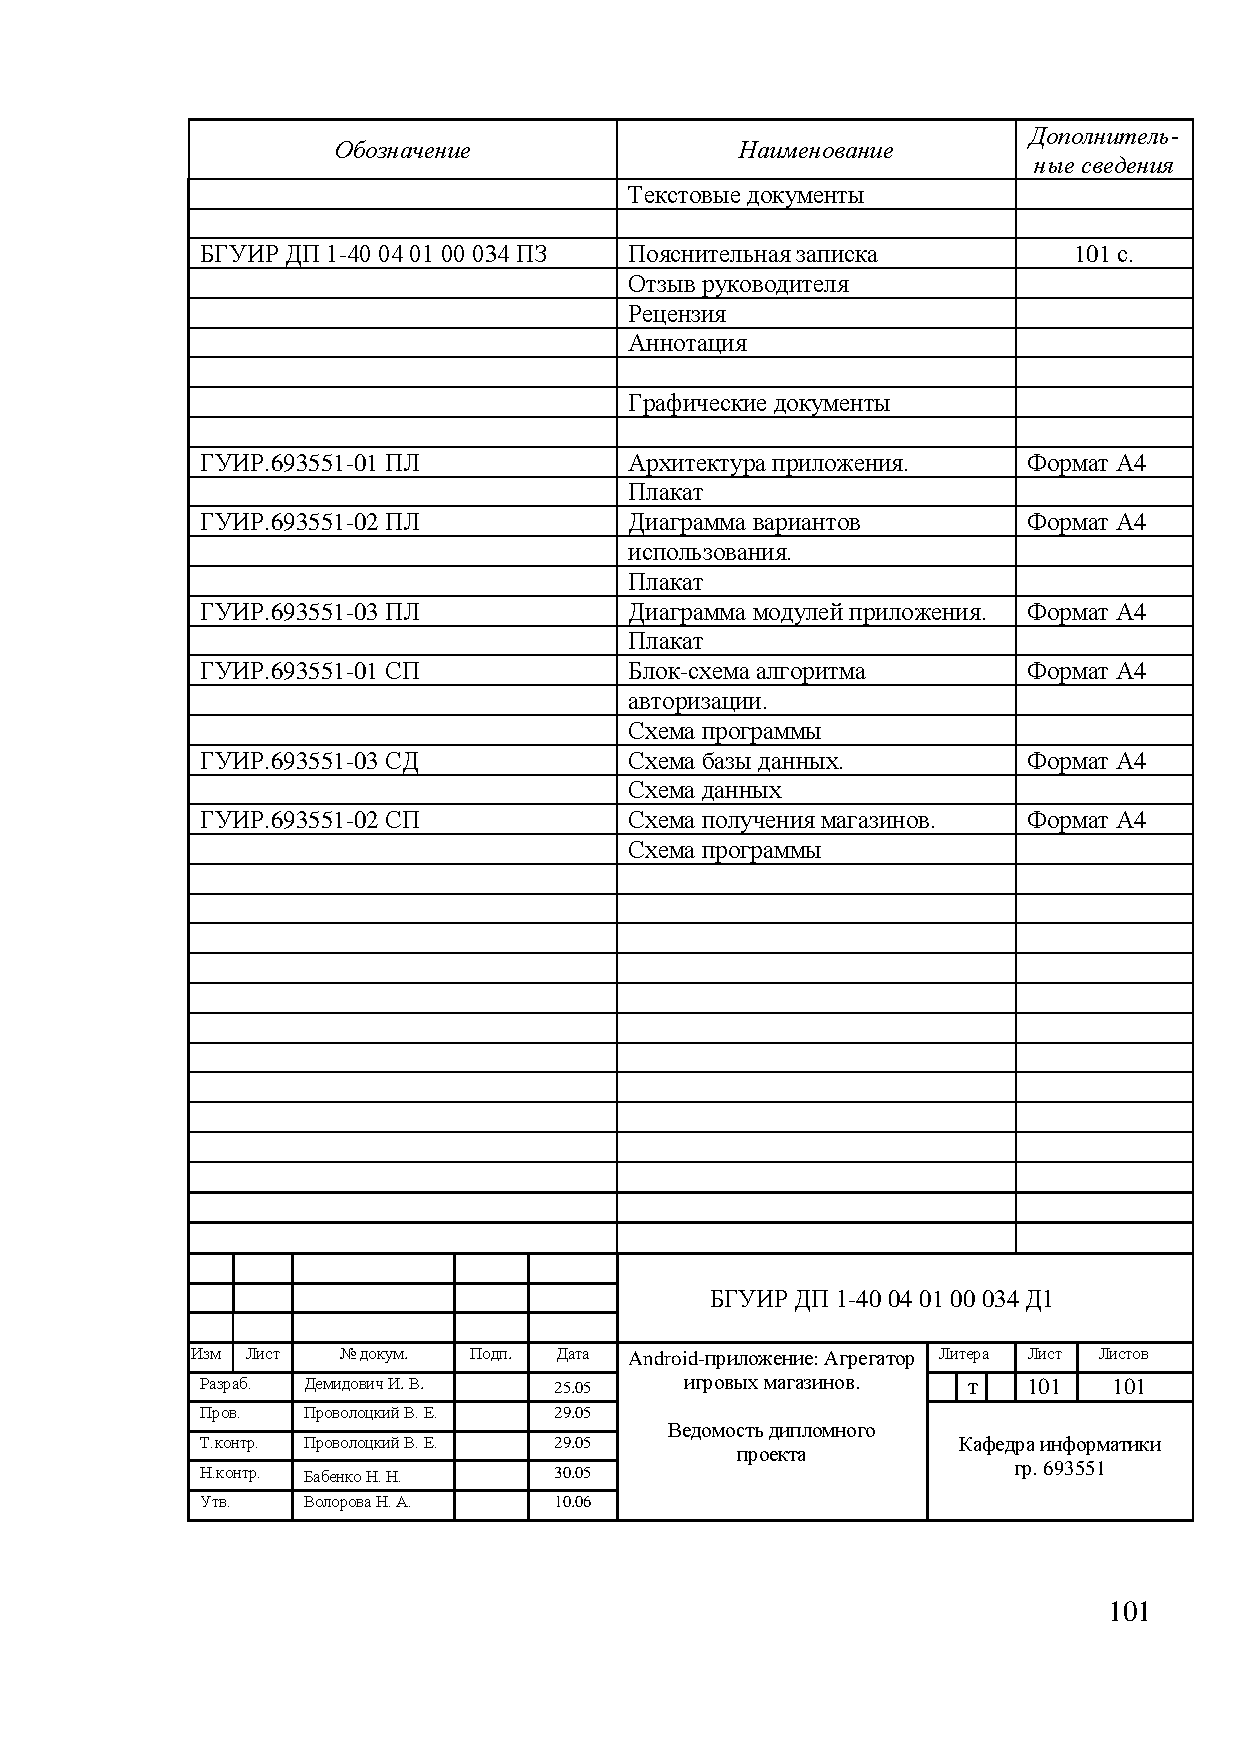
\includepdf[pages={1}]{end.pdf}

% \includepdf позволяет включить в результирующий pdf документ часть другого pdf документа, сделанного
% например не с помощью TeX. Бывает полезно, если какие-то диаграммны нарисованы, например, с помощью 
% Microoft Office и сохранены в pdf.
%\includepdf[pages={-}]{documents_list.pdf}

\end{document}